\clearpage
\section{Event selection}
\label{sec:event-selection}

In the following section we detail the event level selection applied in this analysis. We have seen in~\ref{sec:search-strategy} that we refer to three categories in this analysis: dimuon category, and exclusive track category for each lepton flavor. We summarise the preselection in~\ref{sec:preselection}, then the selection that defines each category in~\ref{sec:category-selection}, and finally the multivariate selection for each category in~\ref{sec:event-bdt}.

\subsection{Baseline selection}
\label{sec:preselection}

We have reviewed some of the base selection that is common to all categories in~\ref{tab:base-selection}. We reiterate reasons for these selections here in additional to other event level selections.

\begin{itemize}

\item $\mht\geq220\GeV$ and $\MET \geq 140\GeV$ cuts intend to boost sensitivity by rejecting \gls{sm} background, as well as to operate in the acceptance regime of the MET trigger, as described in~\ref{sec:trigger}. It is especially efficient in rejecting \gls{qcd} background, since it does not produce real \MET. Any \MET apparent in \gls{qcd} is due to jet energy miss measurements. The reason we are cutting harder on \mht rather than \MET is that \mht sums jets with $\pt>30\GeV$ and is blind to objects with $\pt<30\GeV$. Since we rely in our background estimation on jets with \pt in the range of $[15,30]\GeV$, \mht is more appropriate than \MET since it does not introduce a bias in the data-driven background estimation methods. The two observables are highly correlated though, and describe similar physics.

\item $\njets \left( \pt \geq 30\GeV\, \mathrm{and}\, \abs{\eta} < 2.4 \right) \geq 1$. We are requiring at least one jet in the event, since such an \gls{isr} jet gives a boost to the produced neutralino, thus increasing the missing transverse energy and with it the sensitivity.

\item $\nbjets \left( \pt \geq 30\GeV\, \mathrm{and}\, \abs{\eta} < 2.4 \right) = 0$. We are vetoing any \PQb-tagged jet. Our signal does not contain real \PQb-tagged jets. This veto is efficient in rejecting background from \ttbar, in which the \PQb quarks arise from a \PQt quark decay.

\item $\mindphimhtjets$  $ > 0.4$. Since we are requiring an \gls{isr} jet in the event, we expect the the \gls{mht} to point in the opposite direction of the jet, or at least in an angel close to $\pi$. Events with multiple jets in the \gls{sm} background such as arising from \gls{qcd} will not exhibit such a feature. Therefore this cut reduces \gls{qcd} background.

\item veto events with isolated loose-ID lepton having $\pt\geq 30\GeV$. Lepton can be either muon or electron. Our signal does not have high-\pt leptons, as we have seen in~\ref{sec:signal-signature}.

\item $0.4<\mll<12 \GeV$. Our signal resides in an invariant mass window with an edge at the mass difference between \neutt and \neuto. This is a relatively loose cut that is expected to further be tightened by the boosted decision tree.

\end{itemize}

We have already seen the object level selection in~\ref{sec:object-selection}. For the sake of completeness we reiterate them here. The electrons in the analysis require to pass the following selection (see also~\ref{sec:object-selection-electrons}):

\begin{itemize}

\item $5 \leq \pt \leq 15\GeV$
\item $\abs{\eta} < 2.5$
\item pass jet isolation
\item loose ID

\end{itemize}

The muons in the analysis require to pass the following selection (see also~\ref{sec:muon-selection}):

\begin{itemize}

\item $2 \leq \pt \leq 15\GeV$
\item $\abs{\eta} < 2.4$
\item pass jet isolation
\item medium ID

\end{itemize}

\subsection{Category selection}
\label{sec:category-selection}

The analysis has two main categories: dilepton and exclusive track category. The dilepton category has two leptons, while the exclusive track category has a single lepton and a track that has not been identified as a lepton. The dilepton category includes only one flavor, namely muons, while the exclusive track category has both electrons and muons flavored leptons. Selection for the dilepton category is listed in~\ref{sec:dilepton-selection} and for the exclusive track category in~\ref{sec:exclusive-track-selection}.

\subsubsection{Dilepton selection}
\label{sec:dilepton-selection}

In the dilepton category we have two reconstructed and identified muons. The following lists the selections:

\begin{itemize}

\item $N_\mu = 2$ opposite charge passing the muons selection.
\item $\pt(\mu_2)\leq 3.5\GeV$ or $\DR(\mu_1,\mu_2) < 0.3$. This requirement makes this analysis orthogonal to the \gls{sos} analysis~\cite{sos}.
\item event level BDT cut of $\mathrm{BDT} > 0$. This is the main method of selecting signal events while rejecting the \gls{sm} background. See~\ref{sec:event-bdt} for details.
\item $\DR(\mu_{1,2},\text{leading jet}) > 0.4$. The leptons should not be inside the \gls{isr} jet.
\item \PGo, $\PGr^0$ and \JPsi invariant mass vetoes. $\mll \notin [0.75,0.81]\GeV,\,\mll \notin [3,3.2]\GeV$.
\end{itemize}

\subsubsection{Exclusive track selection}
\label{sec:exclusive-track-selection}

In the exclusive track category we have one reconstructed and identified lepton (either an electron or a muon) and an exclusive track, \ie, a track that does not match an identified lepton. The track in the event that is picked to act as the misidentified lepton is the one with the maximum score of the track \gls{bdt}~\ref{sec:track-bdt}. The following lists the selections:

\begin{itemize}

\item $N_\ell = 1$ lepton passing the muons selection.
\item track picking BDT cut of $\mathrm{BDT} > 0$. See~\ref{sec:track-bdt}.
\item event level BDT cut of $\mathrm{BDT} > 0$. This is the main method of selecting signal events while rejecting the \gls{sm} background. See~\ref{sec:event-bdt} for details.
\item $\DR(\ell,\text{leading jet}) > 0.4$. The lepton should not be inside the \gls{isr} jet.
\end{itemize}

\subsection{Boosted decision trees}
\label{sec:event-bdt}

In order to reject \glsreset{sm}\gls{sm} background, pick signal events and define \glsreset{sr} \glspl{sr}, in this analysis we employ multivariate method of type \glsreset{bdt}\gls{bdt}. For the dimuon category we train one  \gls{bdt}. For the exclusive track category we train a \gls{bdt} for each lepton flavor and also for the two phases of the tracker detector, \ie, phase 0 and phase 1. That makes five \glspl{bdt} overall.

All \glspl{bdt} use the same structure of 120 trees with a maximum depth of 3, with the TMVA package~\cite{tmva}. The \gls{bdt} training is performed with AdaBoost and GiniIndex separation. We are taking all other values as the defaults set by the TMVA package. 

For the training we take tracks from a pool of our privately produced \FASTSIM signal simulations which were listed in~\ref{sec:signal-simulation} for the signal, and the standard model background simulation listen in~\ref{sec:sm-mc} for the background. For the exclusive track category, since we train for the different phases of the tracker detector, we use 2016 simulations of the signal and standard model background to represent phase 0, and the 2017 ones to represent phase 1. For the dimuon category we use only 2017 simulations to represent both phases with an added systematic uncertainty that results from this choice. 

For the pool of our privately produced \FASTSIM signal simulations, we are selecting the full range of simulated higgsino parameter $\mu$ (or the mass of \PSGcpmDo in case of phase 1), but only the range of \dm we want to be most sensitive to. In phase 0, we select $\dmo\in [0.3,4.3]\GeV$ and $\mu\in [100-130]\GeV$. In phase 1 we select $\dmpm \in [0.3-4.6]\GeV$ and $\mu\in [100-500]\GeV$. The baseline selection listen in~\ref{sec:preselection} has been applied. A subset of the selections listed in~\ref{sec:dilepton-selection} and ~\ref{sec:exclusive-track-selection} is used for the training:

\begin{itemize}

\item $N_\mu = 2 (1)$ opposite charge passing the muons selection for the dimuon category (for the exlusive track category).

\item $\DR(\ell),\text{leading jet}) > 0.4$. 

\item track picking BDT cut of $\mathrm{BDT} > 0$ for the exclusive track category.

\end{itemize}

The training has been done without using \gls{mc} weights, since we found that it gives the result with the least amount of over training that arise due to high weighted \gls{mc} events. The training results in satisfactory performance since the kinematics of the low-\pt leptons is expected to look similar in all \gls{sm} background processes. In the following sections, this fact needs to be taken into account when we look at the training input variables distributions. These distributions are plotted as they are seen by the training algorithm, \ie, without \gls{mc} weights and with signal events taken from a pool of different parameter values as described above. Therefore, the ROC curves cannot be understood as a simple signal efficiency versus background rejection. Every \gls{bdt} output working point results in different signal efficiency depending on the signal parameters values. As we will see later on, we do not use one \gls{bdt} value with a simple cut and count, but rather we are binning the \glspl{sr} in \gls{bdt} output values. We therefore choose to plot the ROC curve with a default cut of 0.0 for the sake completeness. To fully estimate the power of the training, we need to look at the significance when each signal point has been properly weighted together with the \gls{sm} background processes. 

\subsubsection{Dimuon category}

The training samples for the dimuons category contain 4350 signal events and 21842 background events. The training samples are then tested against the test samples of equal size. The distributions of the testing samples overlay on the training samples, as well as the ROC curve, are seen in~\ref{fig:event-bdt-dimuon-output}. No significant over training is observed. 

\begin{figure}[!htb]
\centering
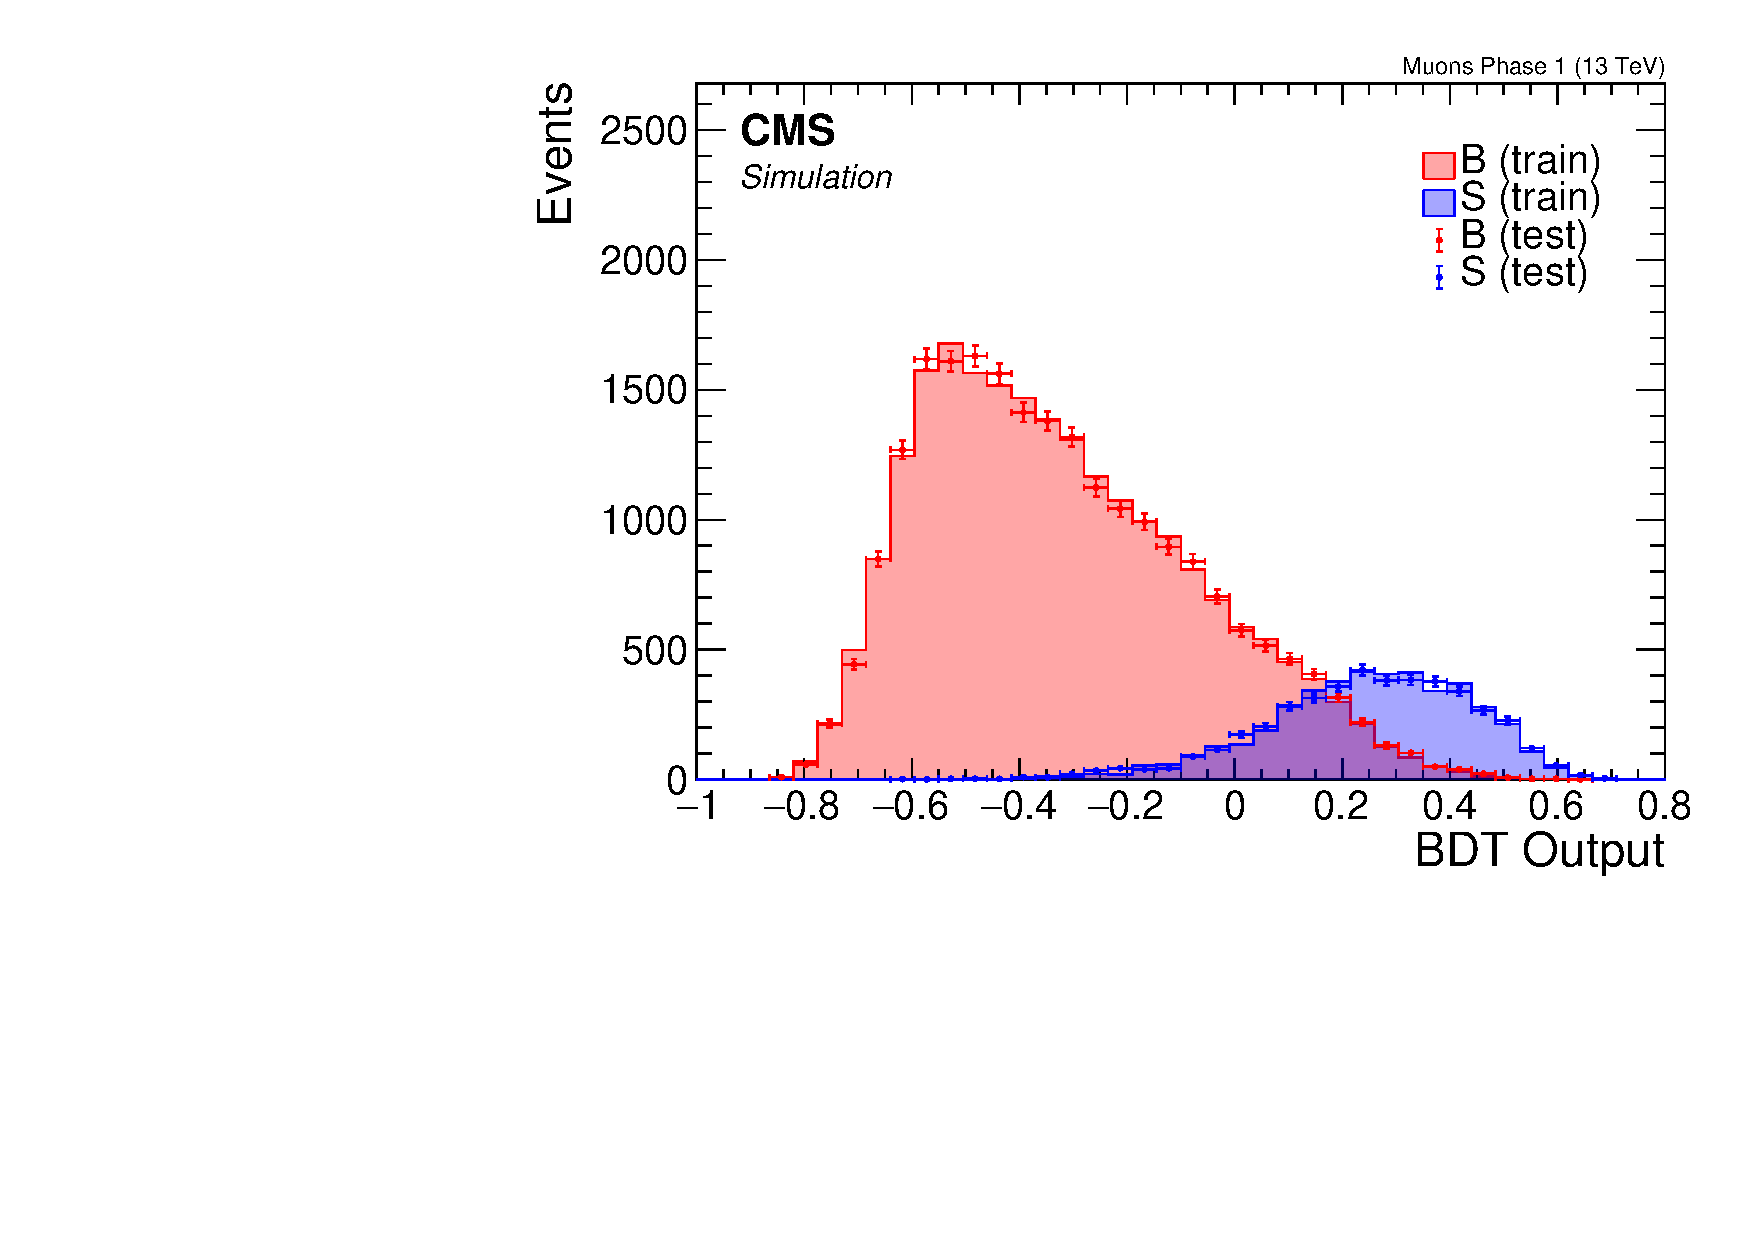
\includegraphics[width=0.48\linewidth]{plots/dimuon_bdt/overtraining_Event_Dilepton_Muons_Phase_1.pdf} \,
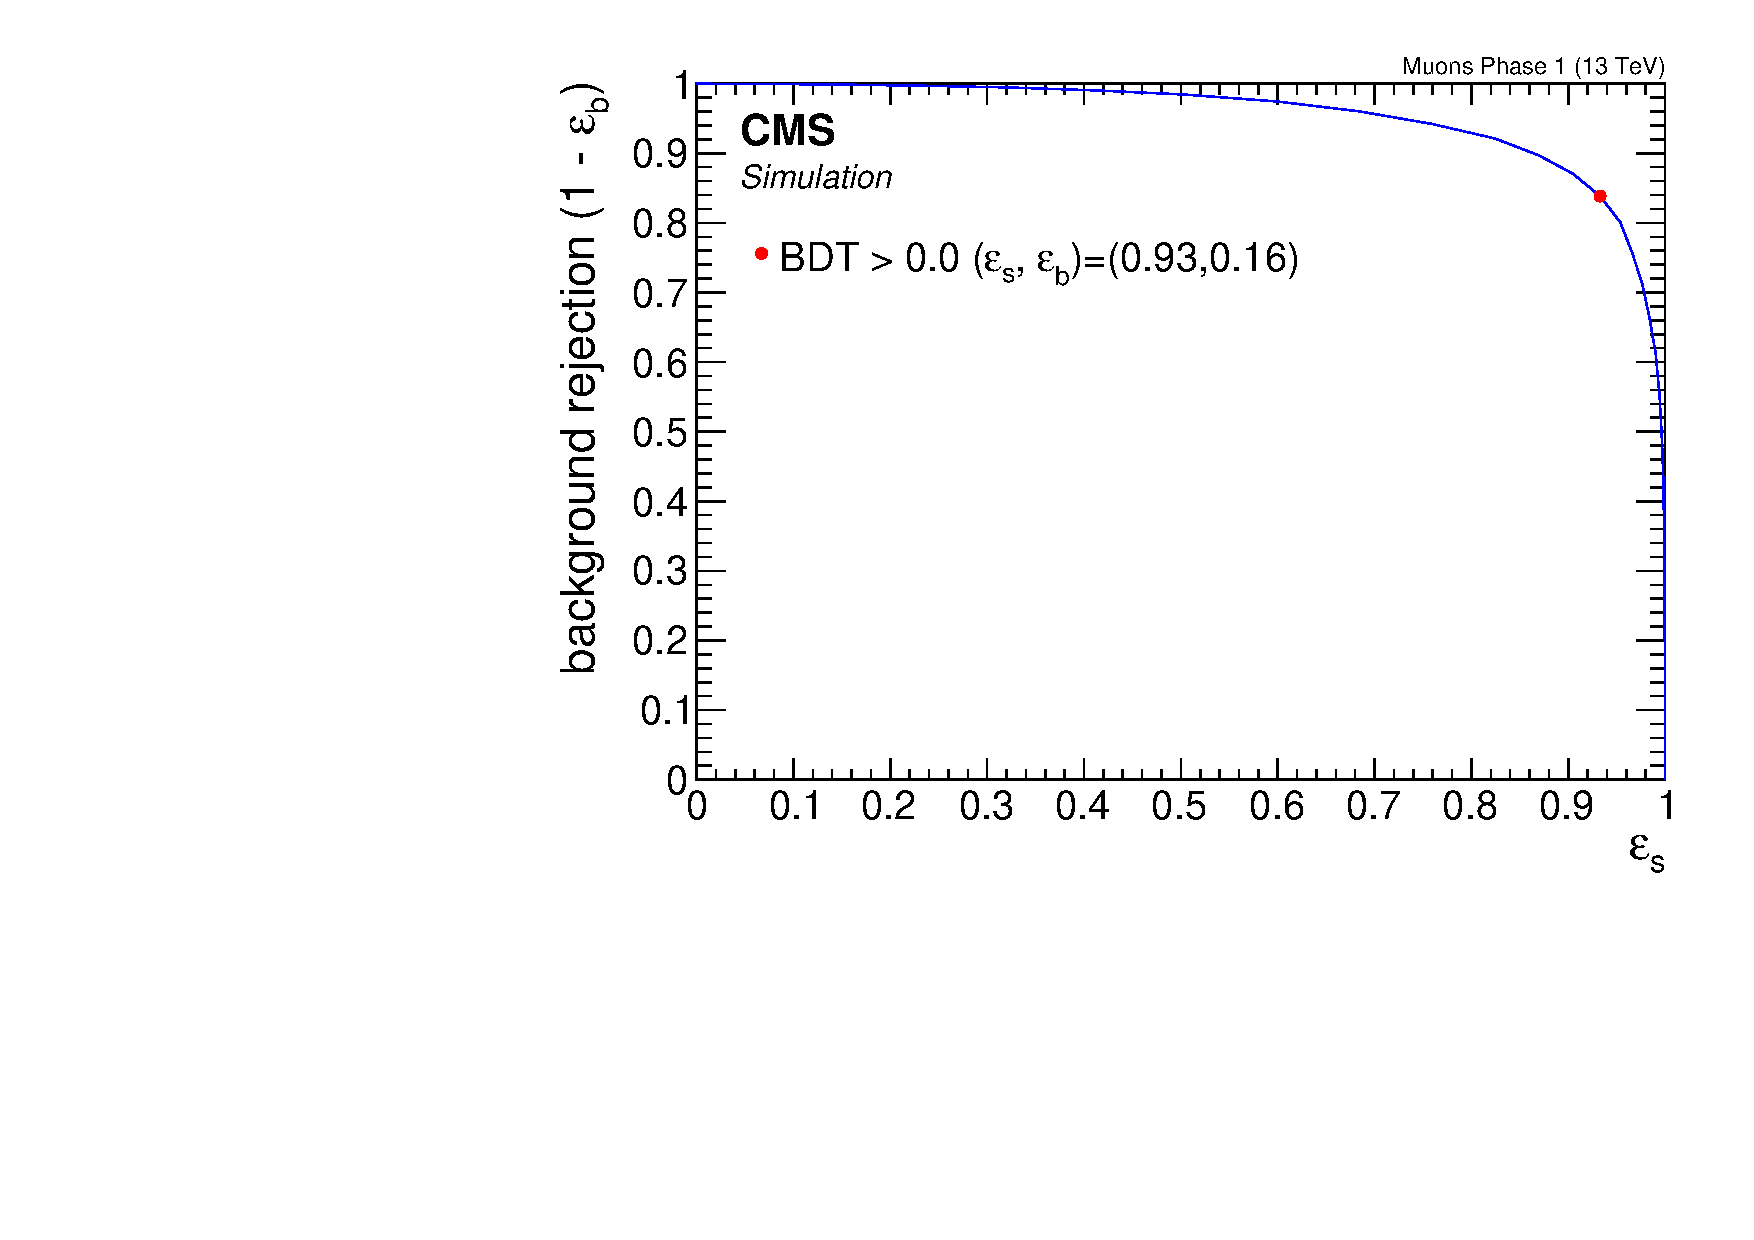
\includegraphics[width=0.48\linewidth]{plots/dimuon_bdt/roc_Event_Dilepton_Muons_Phase_1.pdf} \\


\caption[Dimuon BDT output and ROC curve]{Dimuon BDT output (left) and ROC curve (right).}
\label{fig:event-bdt-dimuon-output}
\end{figure}

The training uses 18 different variable listed in~\ref{tab:dimuon-bdt-variables} in decreasing order of importance ranking.

\begin{table}[!htb]
	\centering
	\label{tab:dimuon-bdt-variables}
		\caption{Dimuon BDT input variables}
		%\vspace{1mm}
			\begin{tabular}{cll} \hline
			Rank & Variable & Description \\ \hline
			1 & $\mll$ & invariant mass \\
			2 & $\pt(\ell_1)$ & leading lepton \pt\\
			3 & \mht & \\
			4 & \HT & \\
			5 & $\DR\left(\ell\ell\right)$ & \\
			6 & $\mindphimhtjets$ & \\
			7 & $\pt(\vec{\ell}_1+\vec{\ell}_2)$ & dilepton \pt \\
			
			8 & $\pt(\text{leading jet})$ & \\		
			9 & $\pt(\ell_2)$ & subleading lepton \pt \\
			10 & $\eta(\ell_1)$ & leading lepton $\eta$ \\
			11 & $m_T(\ell_1)$ & leading lepton transverse mass\\
			
			12 & $\abs{\Delta\phi\left(\ell_2, \htvecmiss \right)}$ & \\
			13 & $\abs{\Delta\phi\left(\ell_1, \htvecmiss \right)}$ & \\			
			14 & $\abs{\Delta\phi\left(\ell\ell \right)}$ & \\			
			15 & $\njets$ & Number of jets \\ 
			16 & $\eta(\text{leading jet})$ & \\
			17 & $\abs{\Delta \eta \left(\ell \ell\right) }$ & \\
			18 & $\mtautau$ & collinear approximation of $\mtautau$\\
			\hline
			\end{tabular}
\end{table}

Distributions of the input variables to the \gls{bdt} training can be seen in~\ref{fig:dimuon-input-distributions}. As mentioned before, the signal is taken from a pool of a range of model points, and events are not weighted to any luminosity or cross section in order to avoid over training. 

\begin{figure}[!htb]
\centering
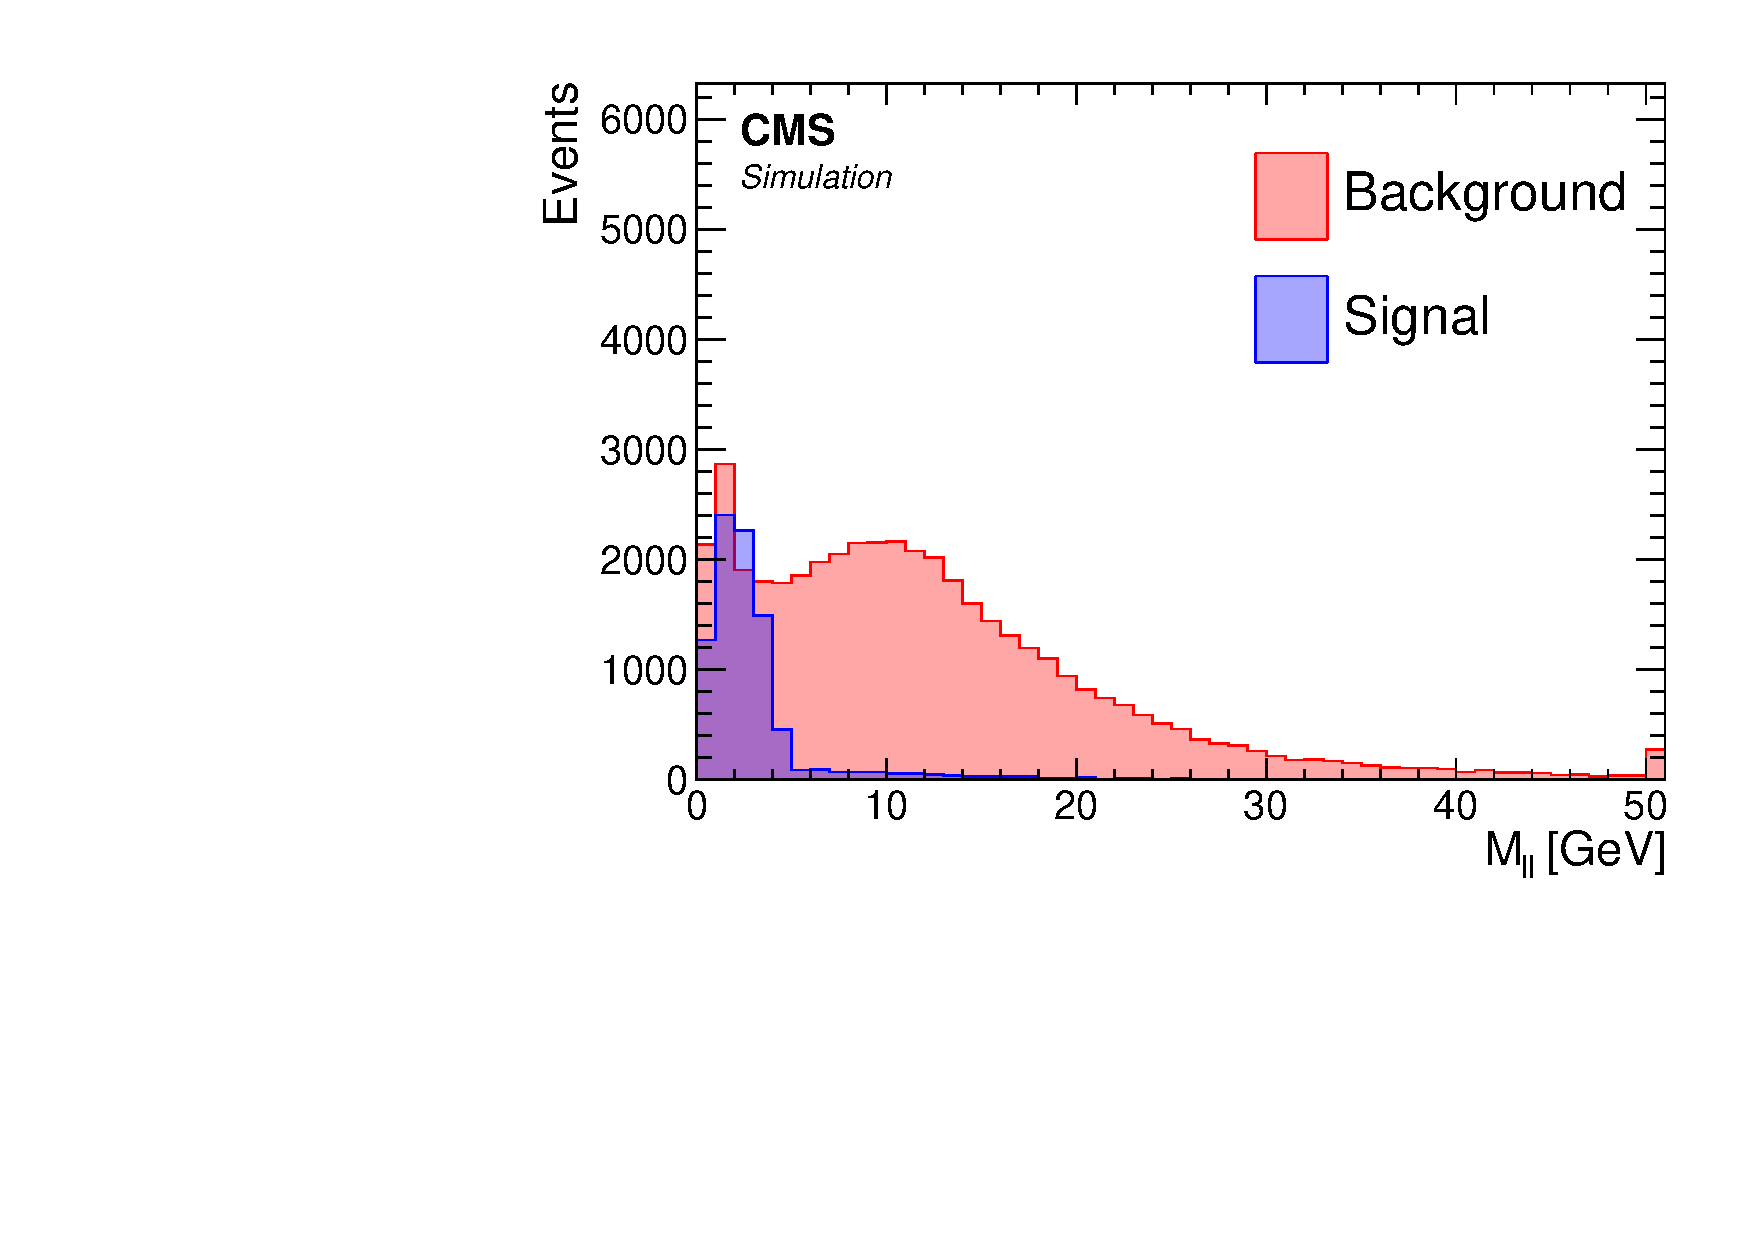
\includegraphics[width=0.32\linewidth]{plots/dilepton_bdt_inputs_muons/none_invMassCorrJetNoMultIso10Dr0.6.pdf} \,
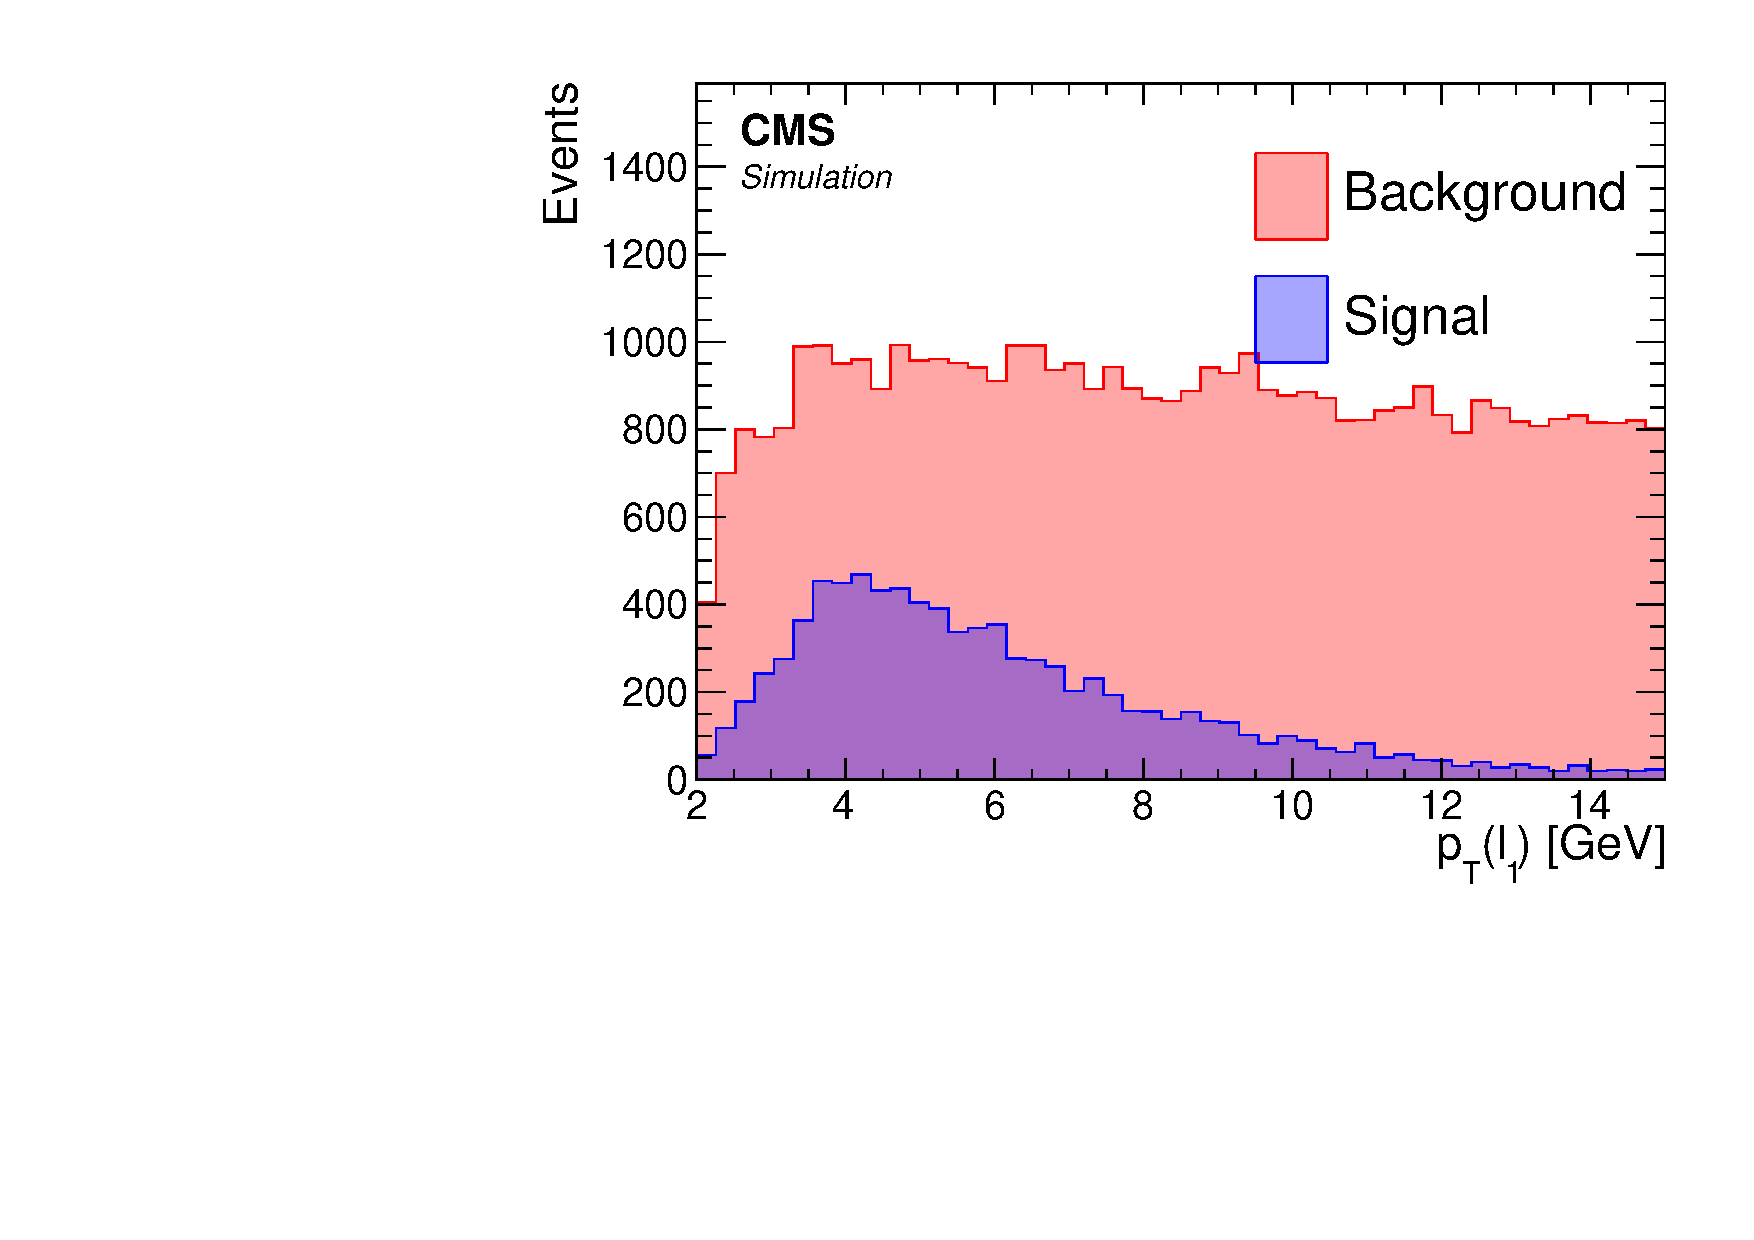
\includegraphics[width=0.32\linewidth]{plots/dilepton_bdt_inputs_muons/none_leptonsCorrJetNoMultIso10Dr0.6_0_.Pt__.pdf} \,
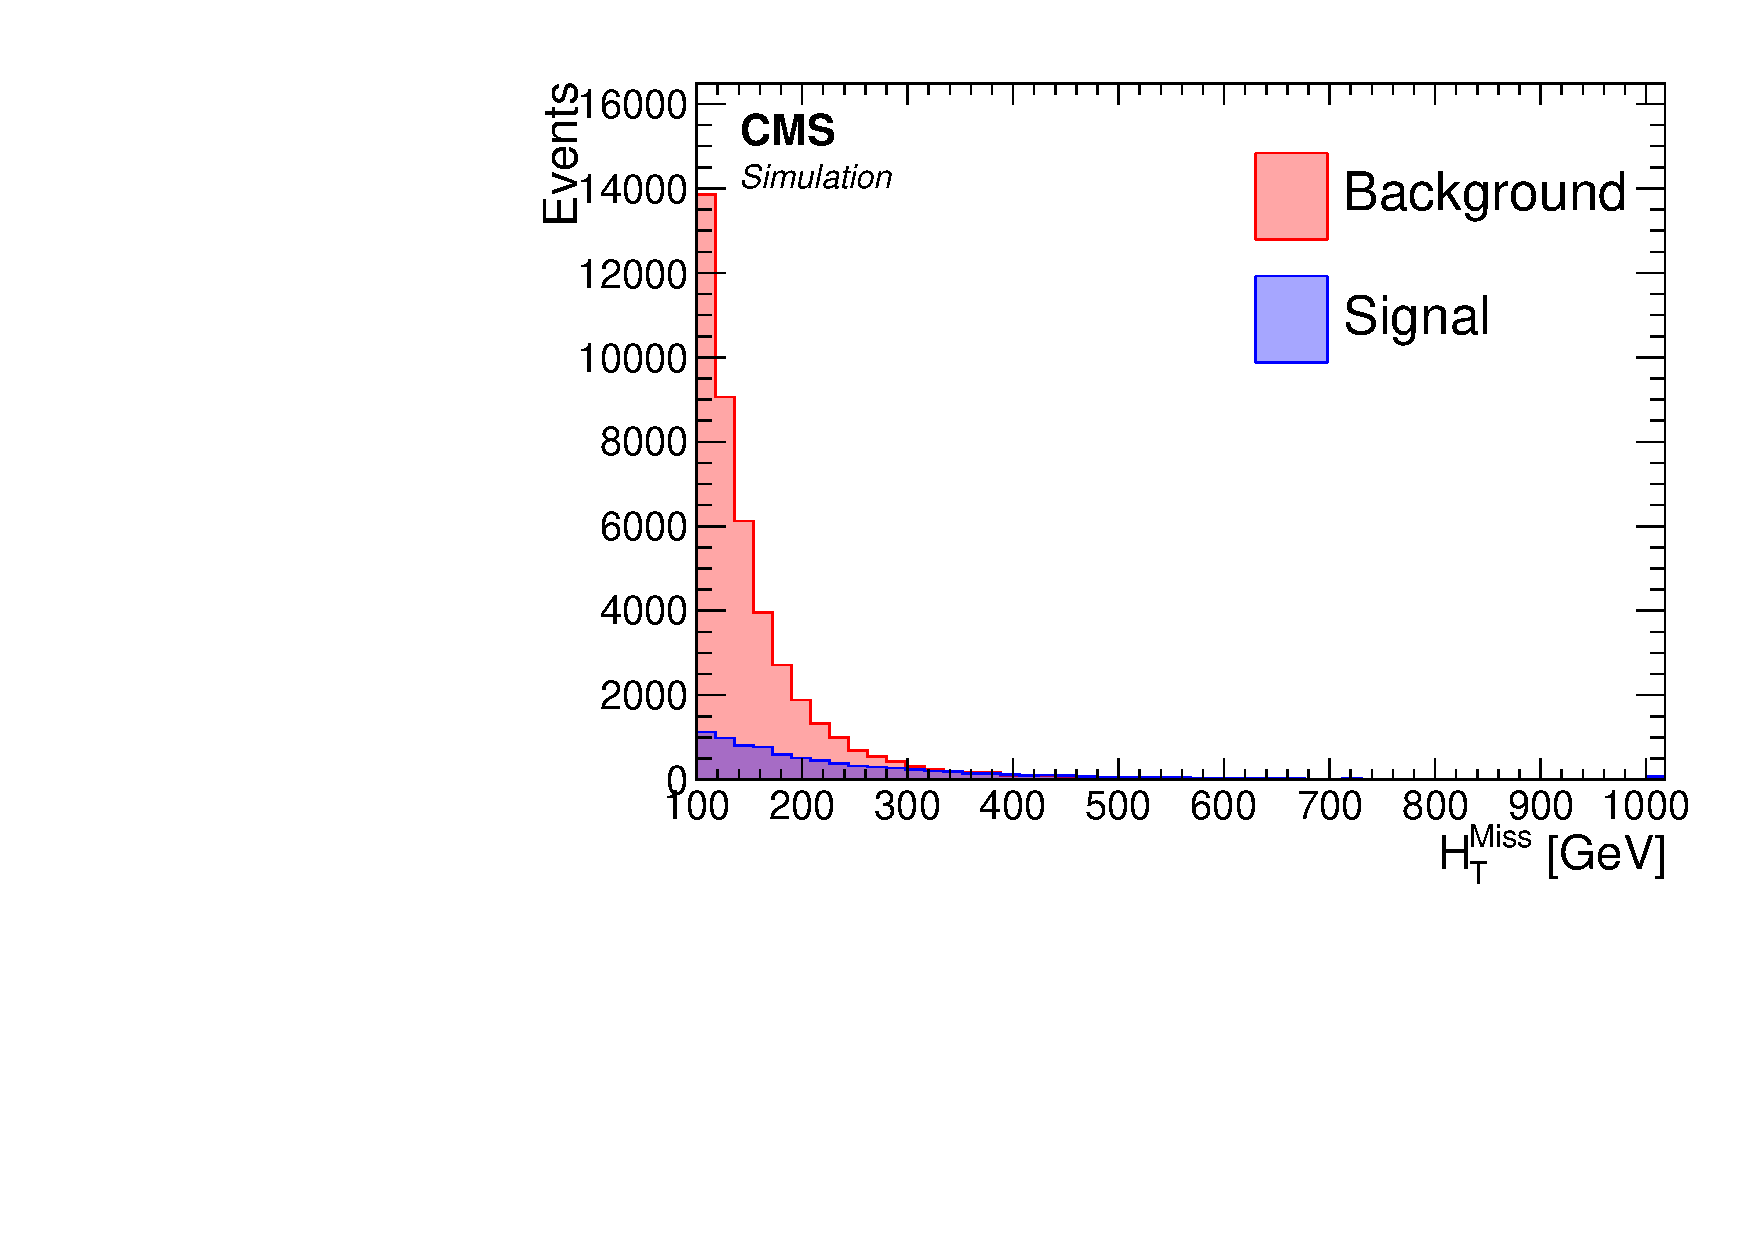
\includegraphics[width=0.32\linewidth]{plots/dilepton_bdt_inputs_muons/none_MHT.pdf}   \\
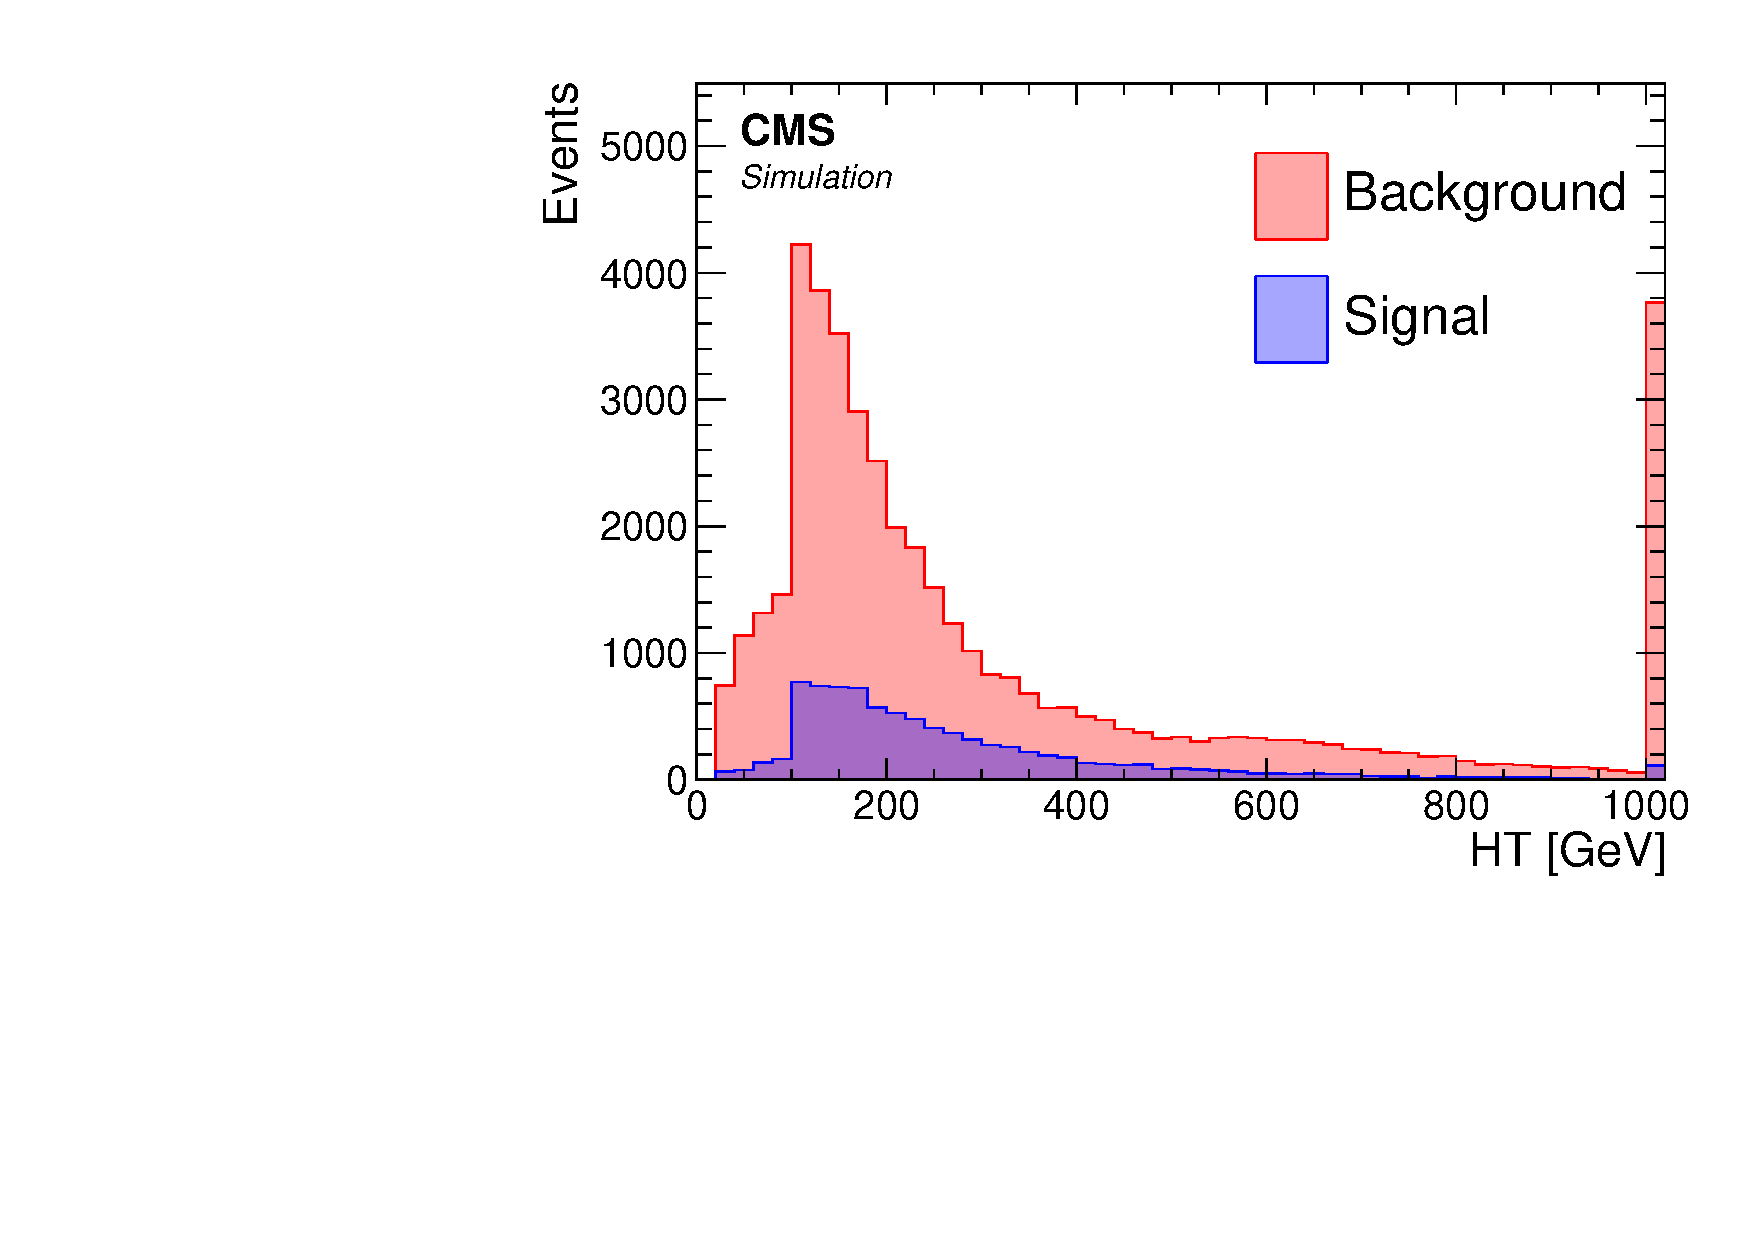
\includegraphics[width=0.32\linewidth]{plots/dilepton_bdt_inputs_muons/none_HT.pdf} \,
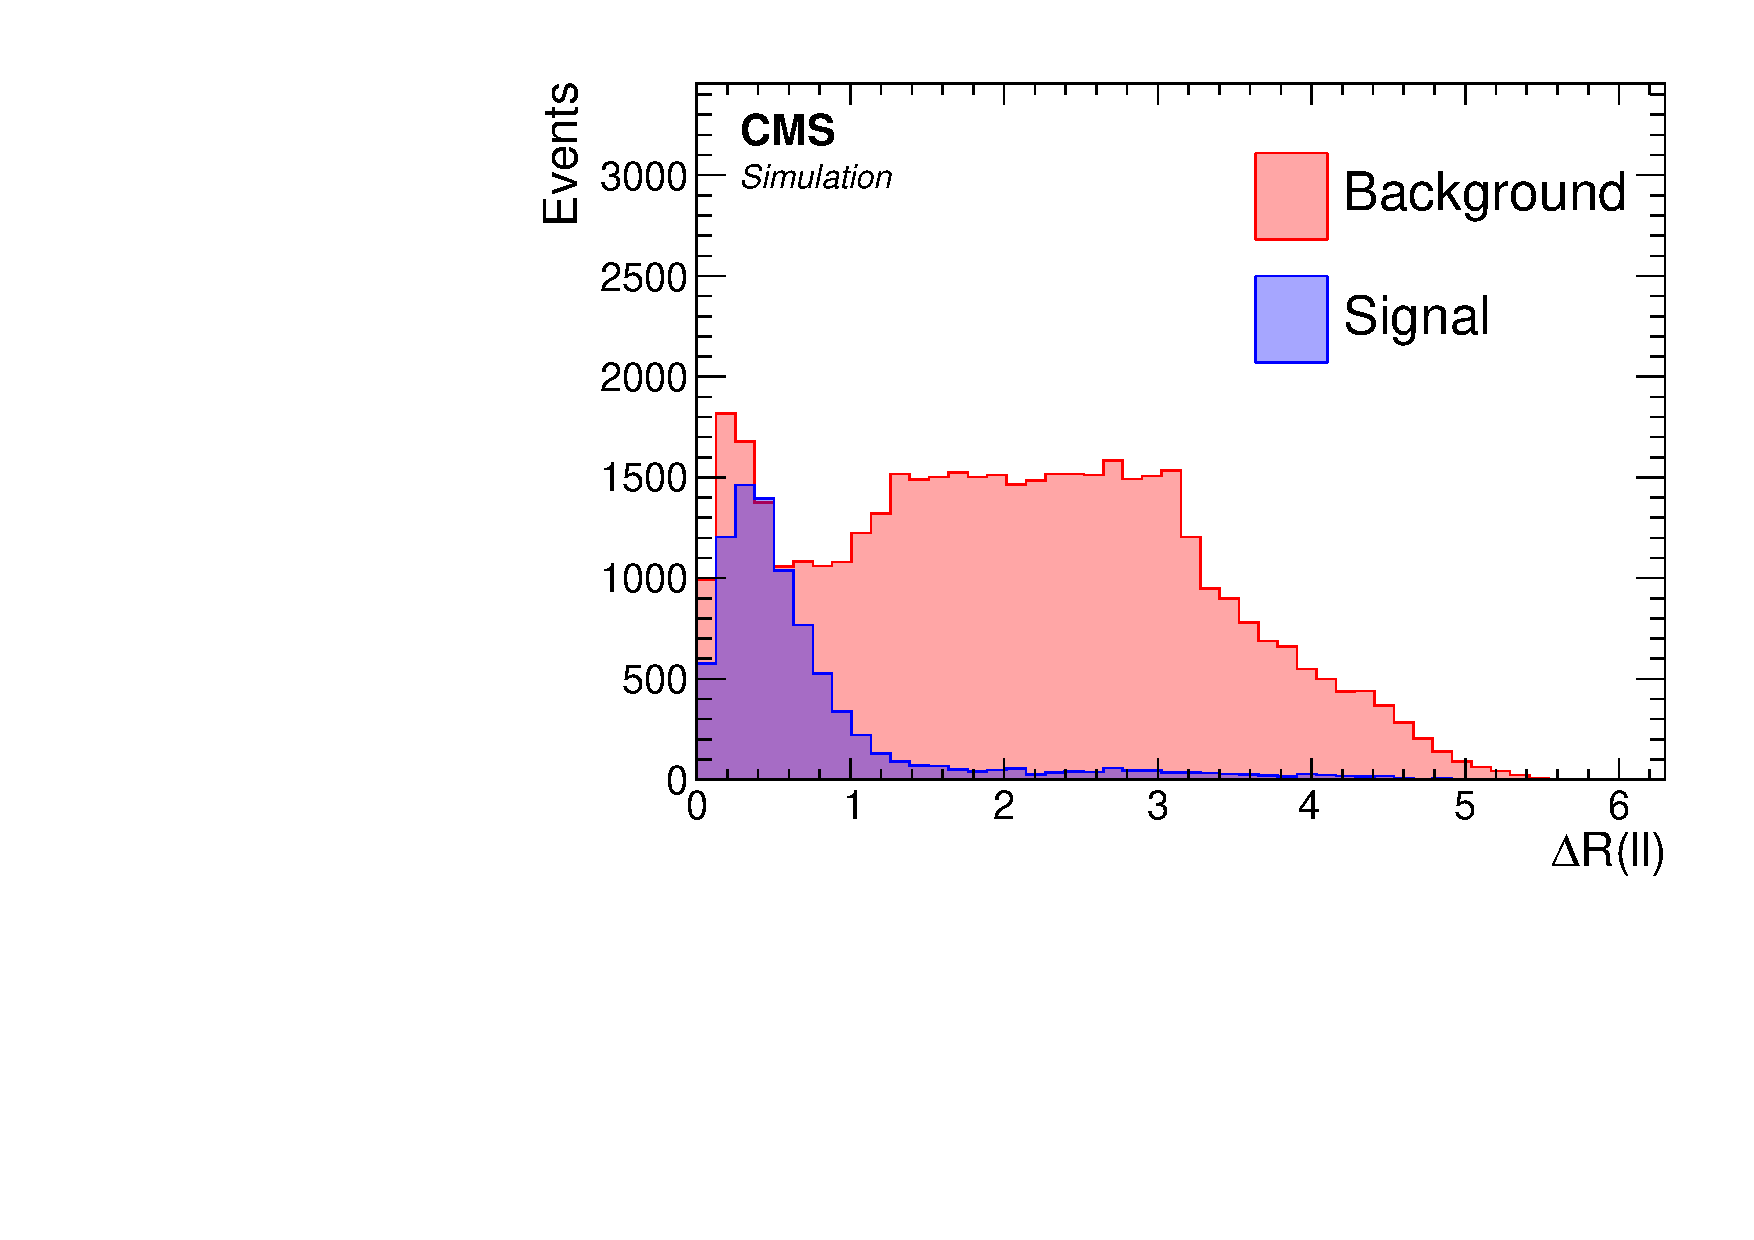
\includegraphics[width=0.32\linewidth]{plots/dilepton_bdt_inputs_muons/none_deltaRCorrJetNoMultIso10Dr0.6.pdf}  \,
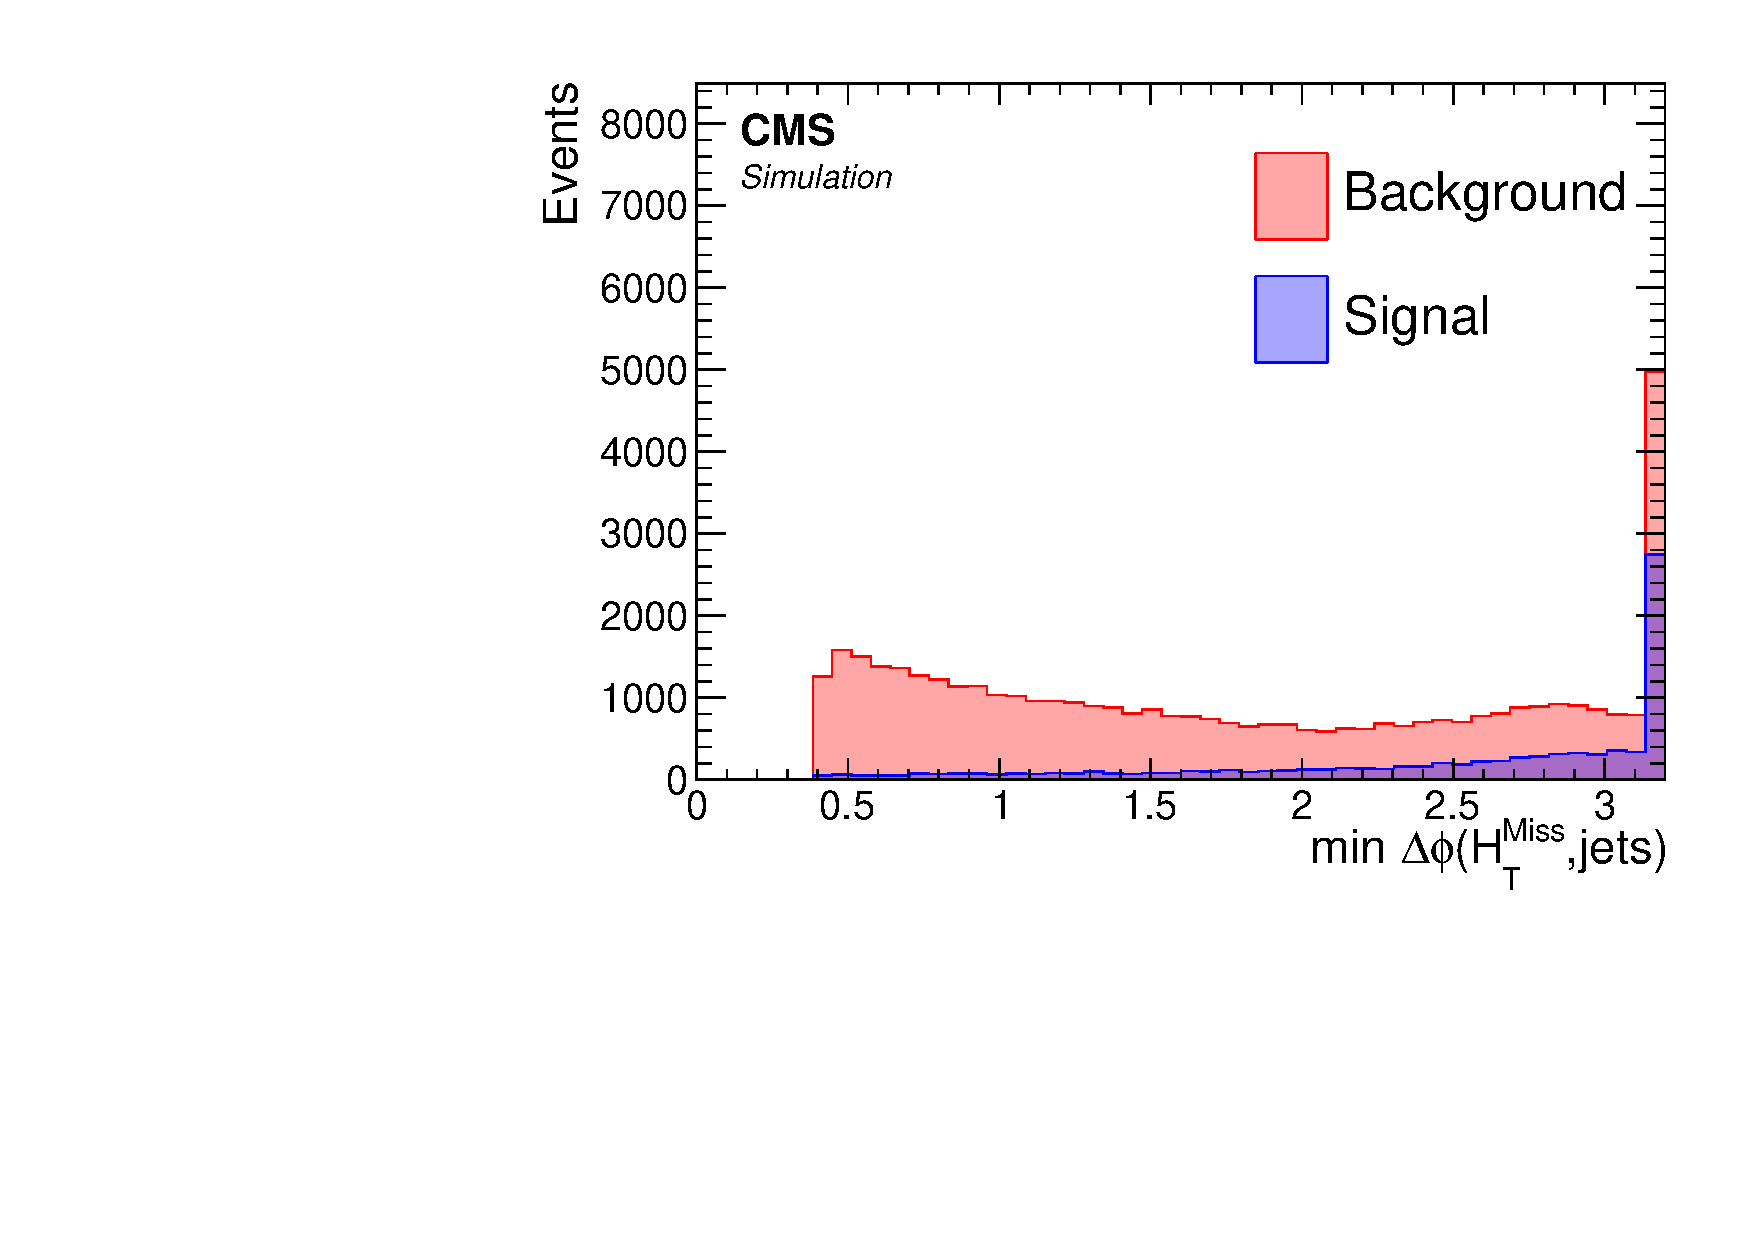
\includegraphics[width=0.32\linewidth]{plots/dilepton_bdt_inputs_muons/none_MinDeltaPhiMhtJets.pdf} \\


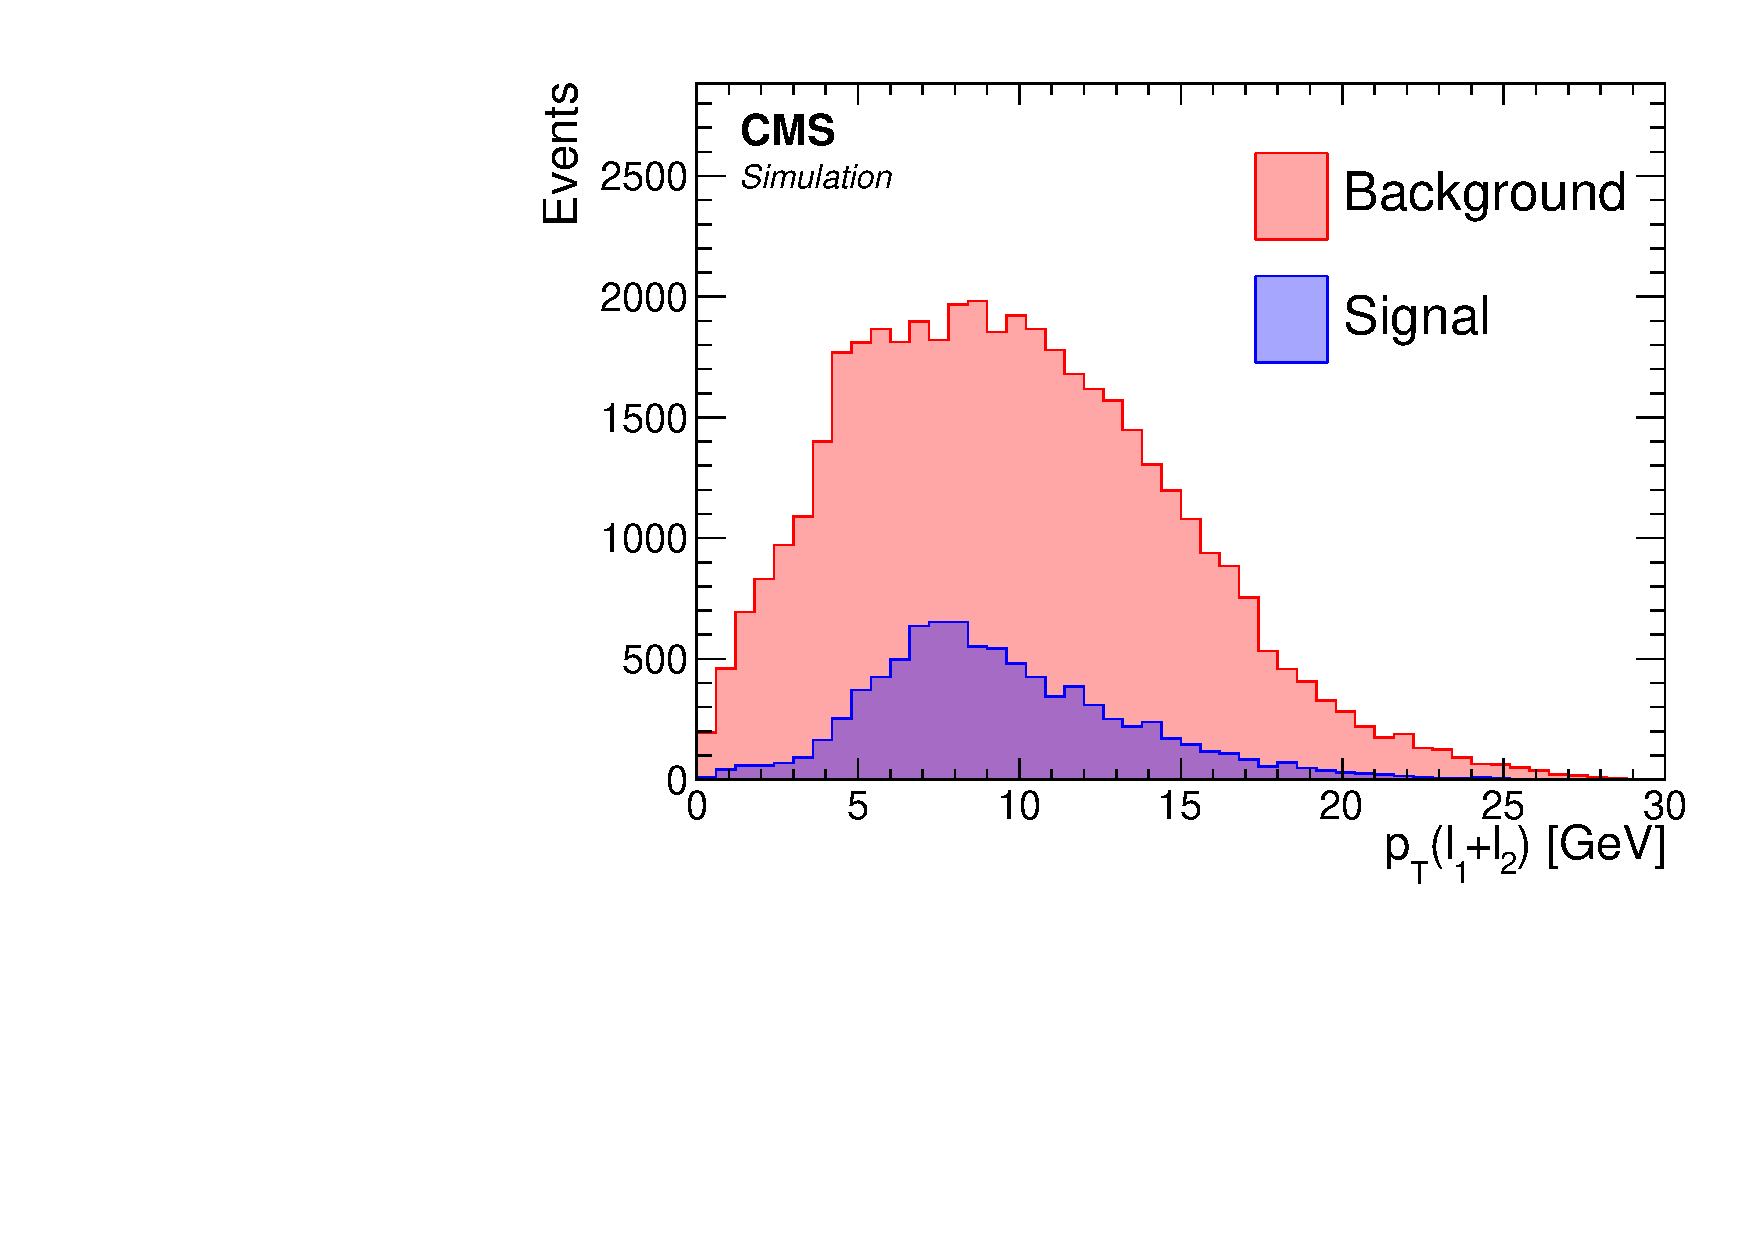
\includegraphics[width=0.32\linewidth]{plots/dilepton_bdt_inputs_muons/none_dileptonPtCorrJetNoMultIso10Dr0.6.pdf} \,
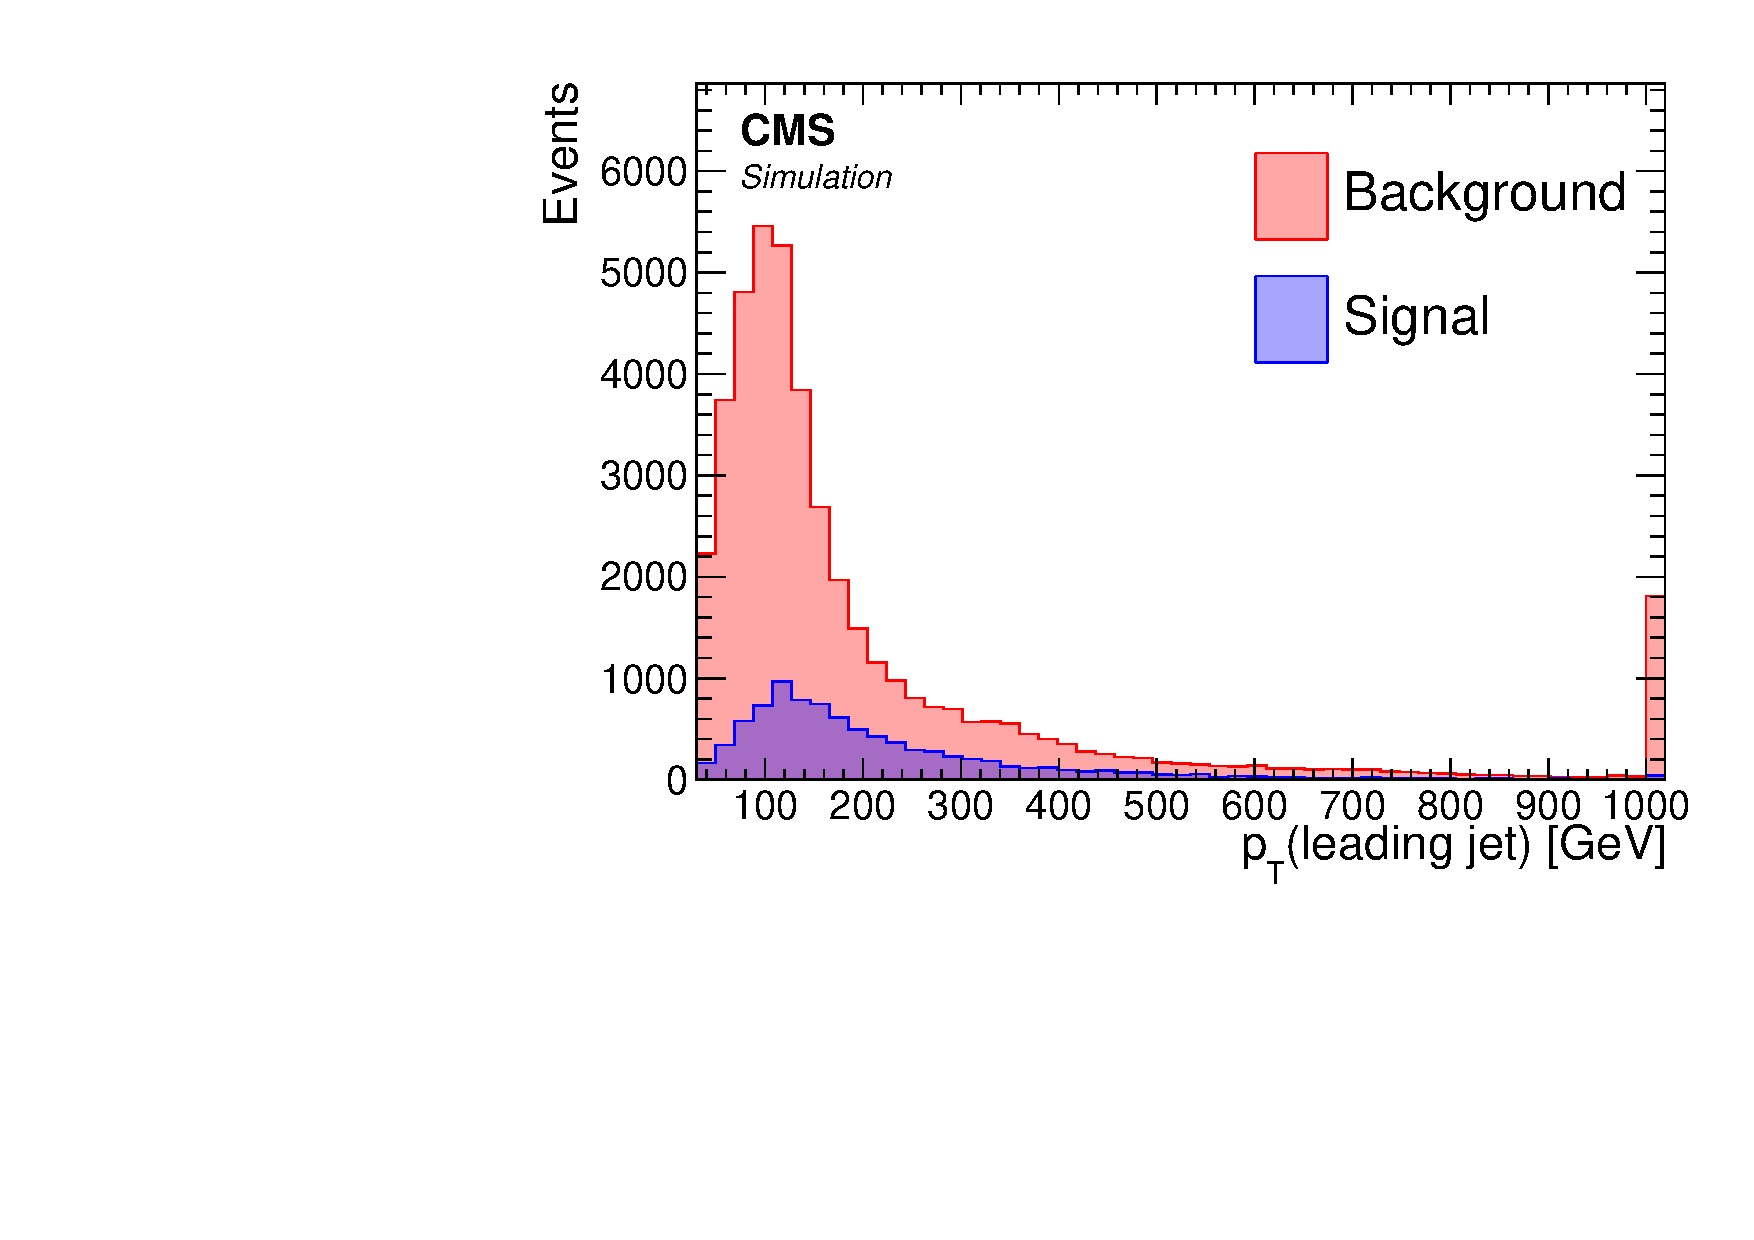
\includegraphics[width=0.32\linewidth]{plots/dilepton_bdt_inputs_muons/none_LeadingJetPt.pdf} \,
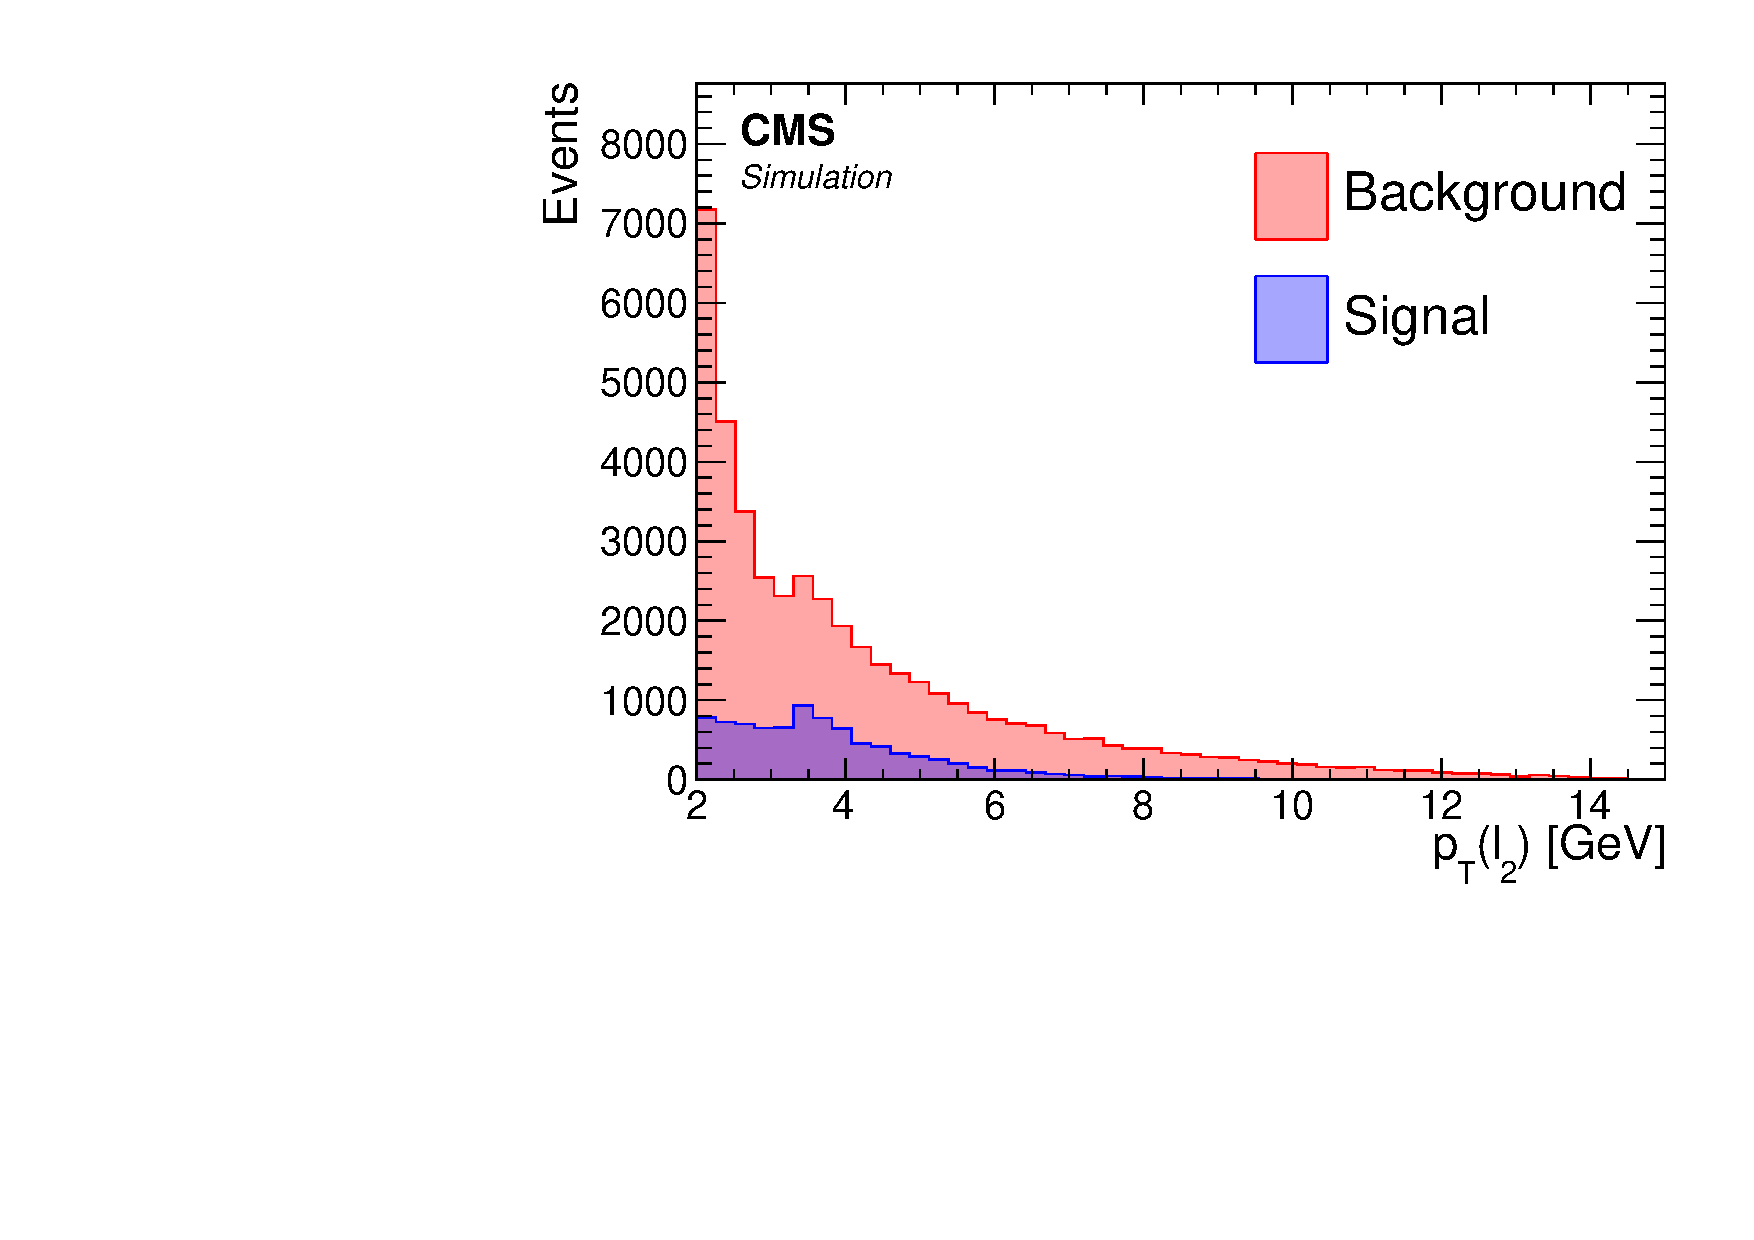
\includegraphics[width=0.32\linewidth]{plots/dilepton_bdt_inputs_muons/none_leptonsCorrJetNoMultIso10Dr0.6_1_.Pt__.pdf}   \\
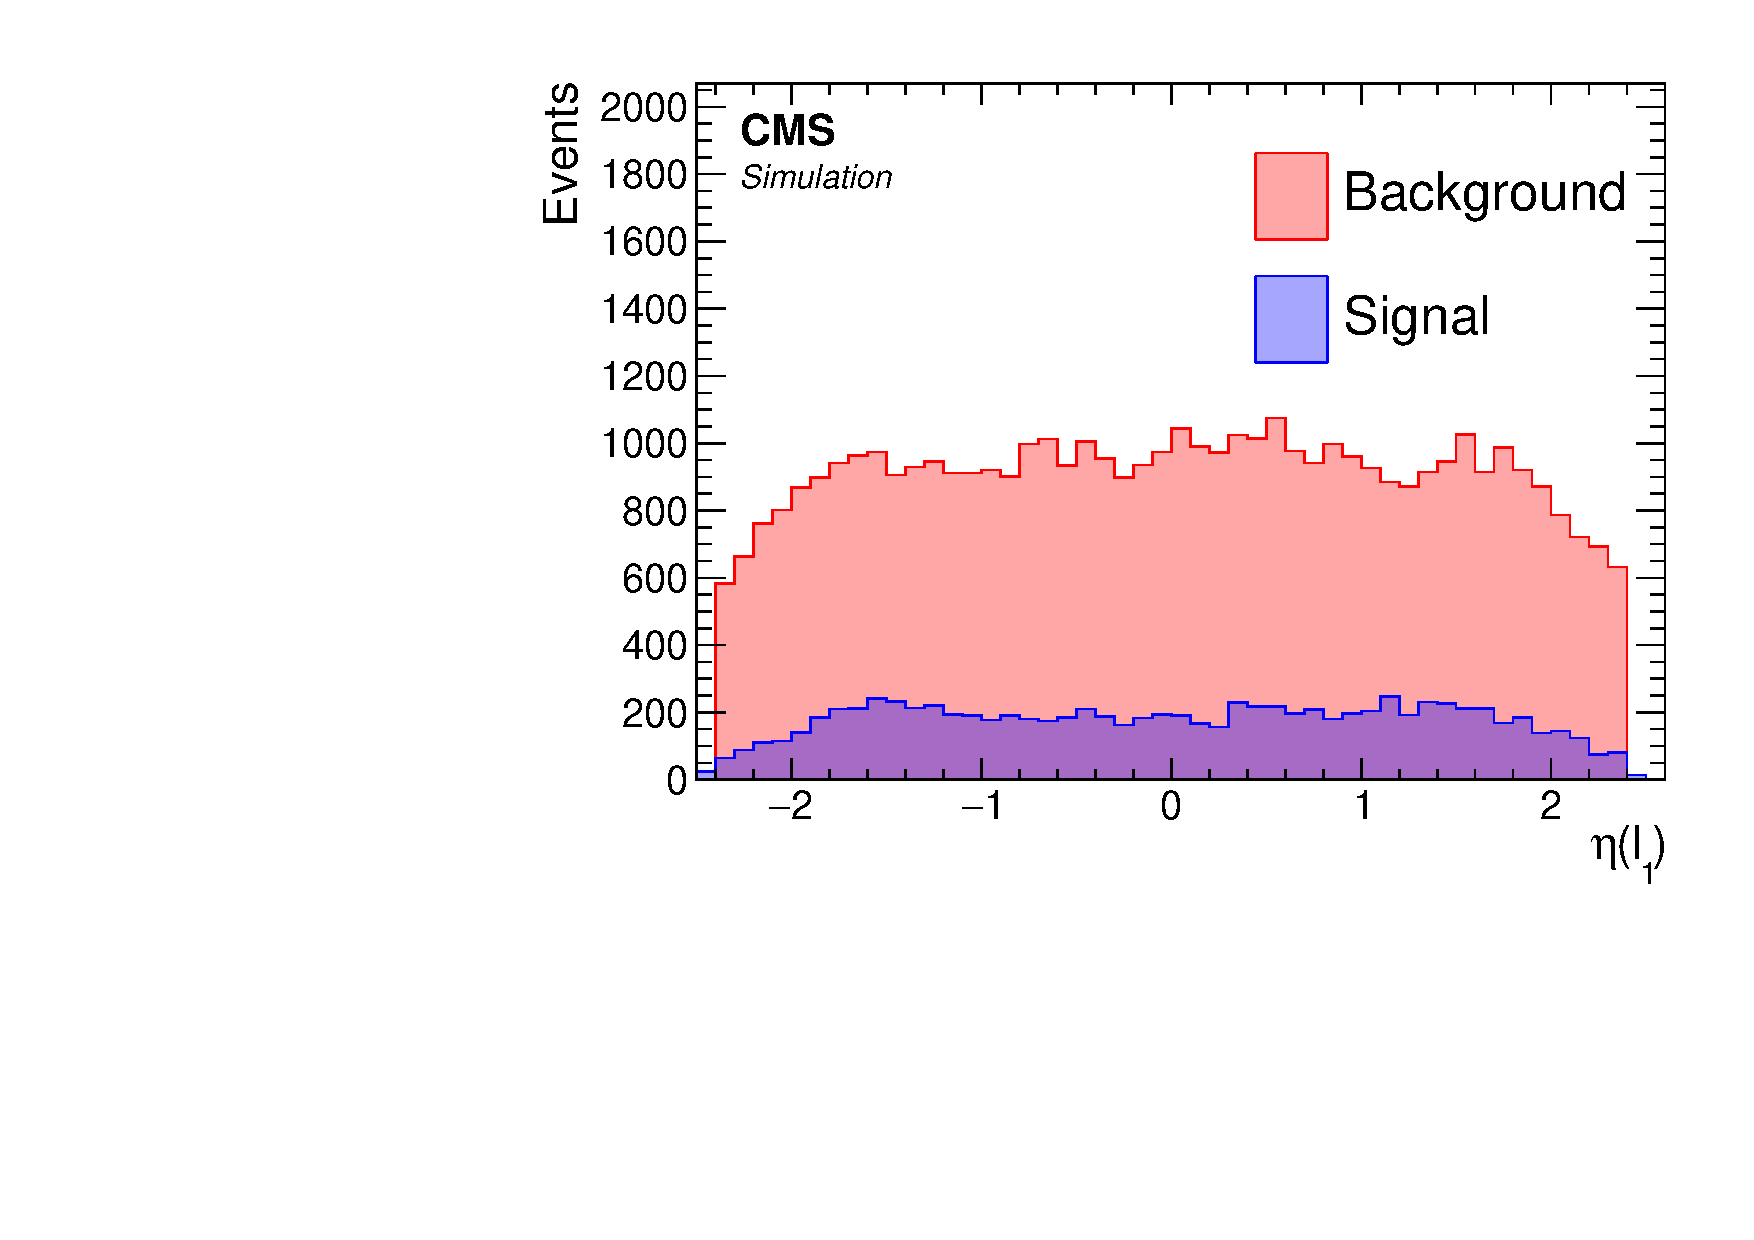
\includegraphics[width=0.32\linewidth]{plots/dilepton_bdt_inputs_muons/none_leptonsCorrJetNoMultIso10Dr0.6_0_.Eta__.pdf} \,
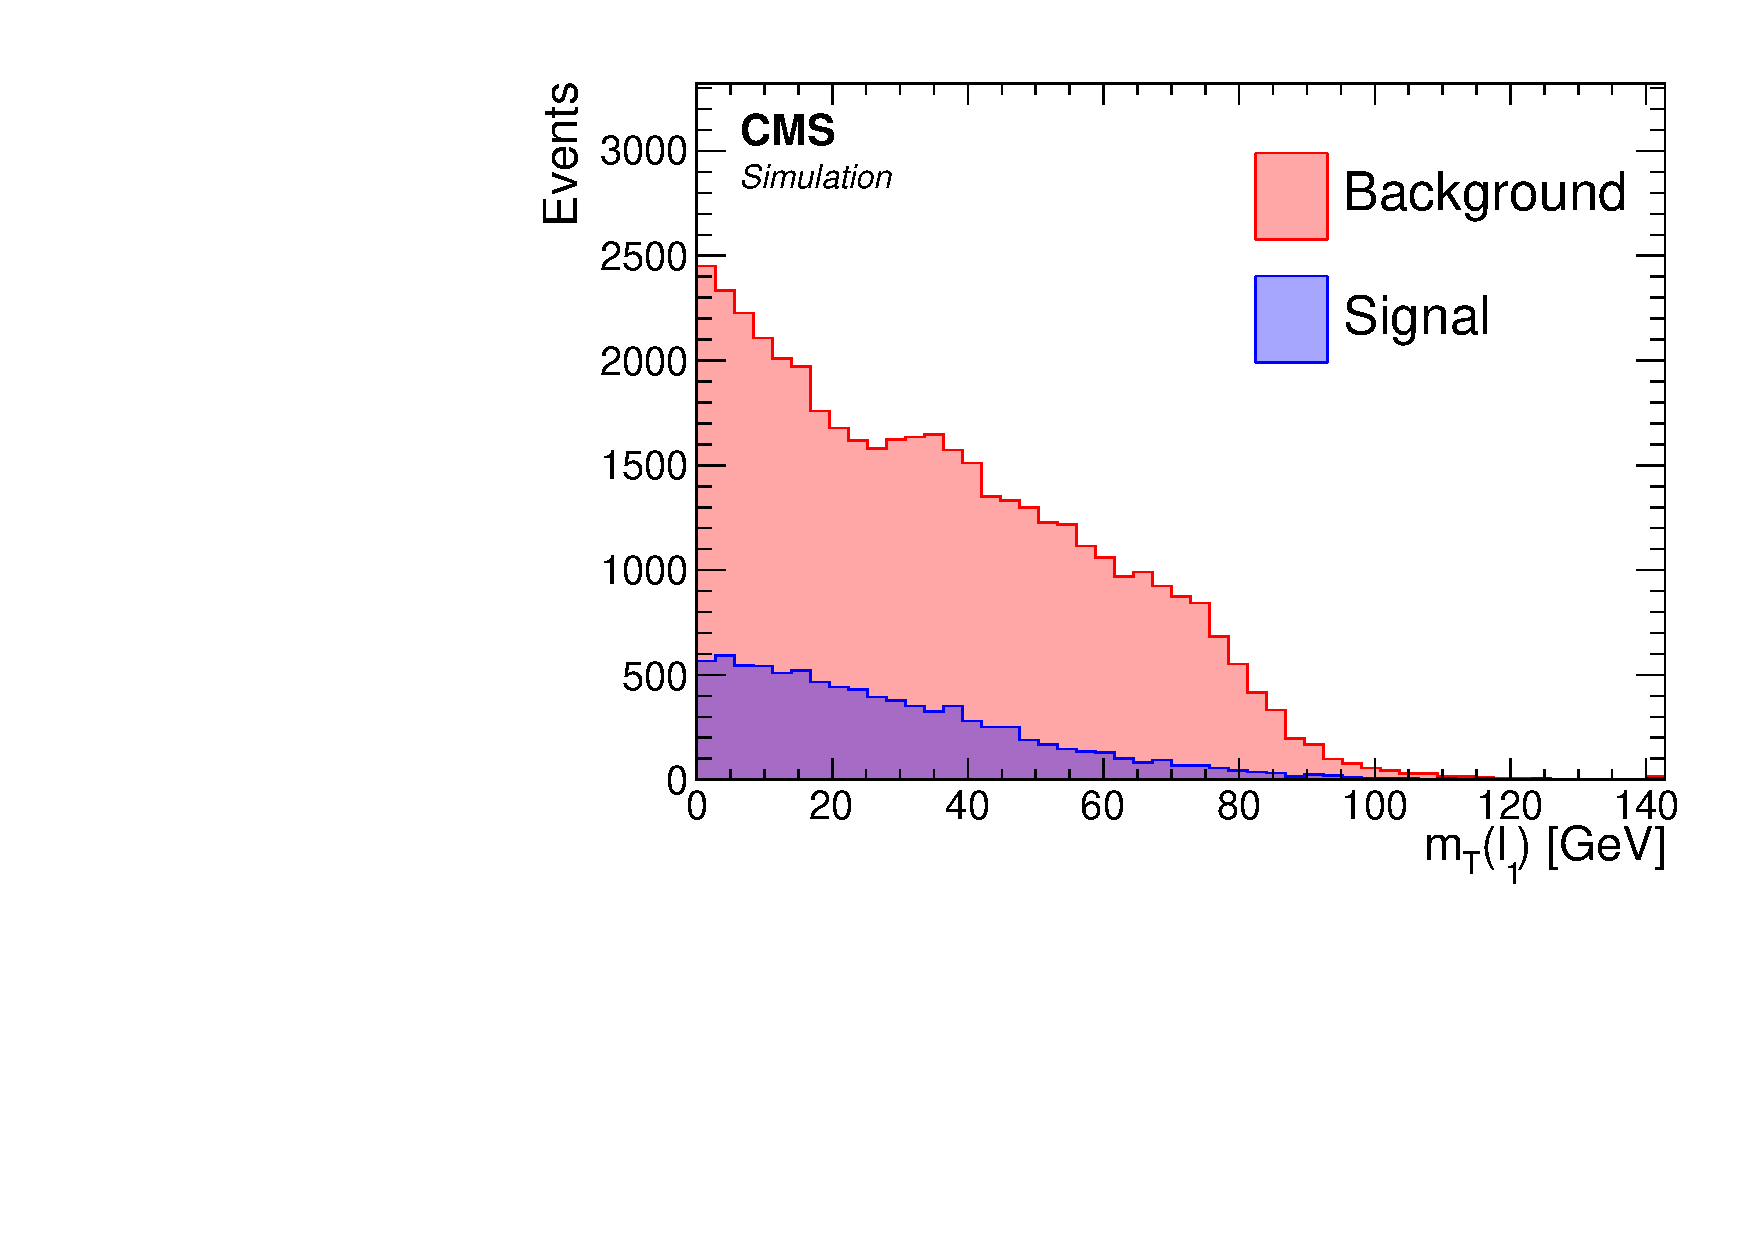
\includegraphics[width=0.32\linewidth]{plots/dilepton_bdt_inputs_muons/none_mth1CorrJetNoMultIso10Dr0.6.pdf}  \,
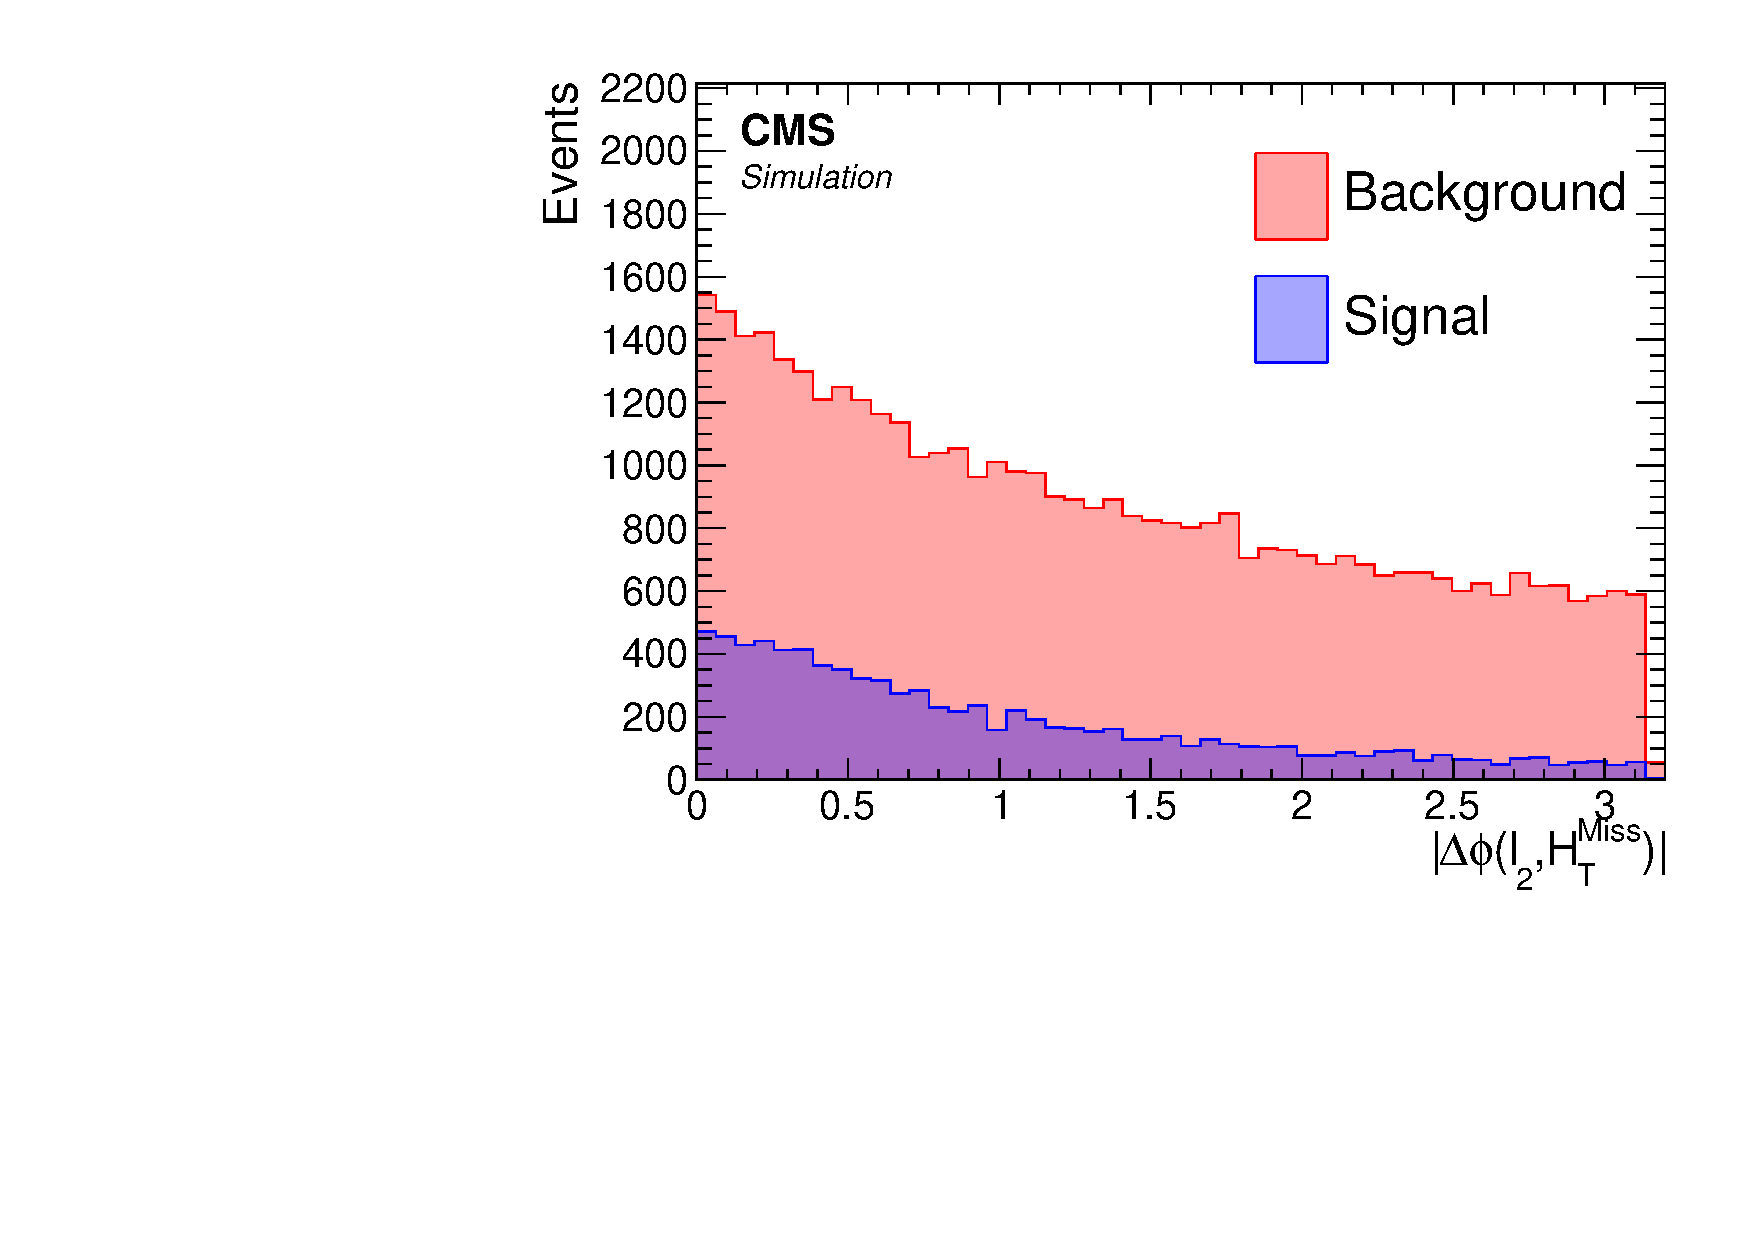
\includegraphics[width=0.32\linewidth]{plots/dilepton_bdt_inputs_muons/none_deltaPhiMhtLepton2CorrJetNoMultIso10Dr0.6.pdf} \\


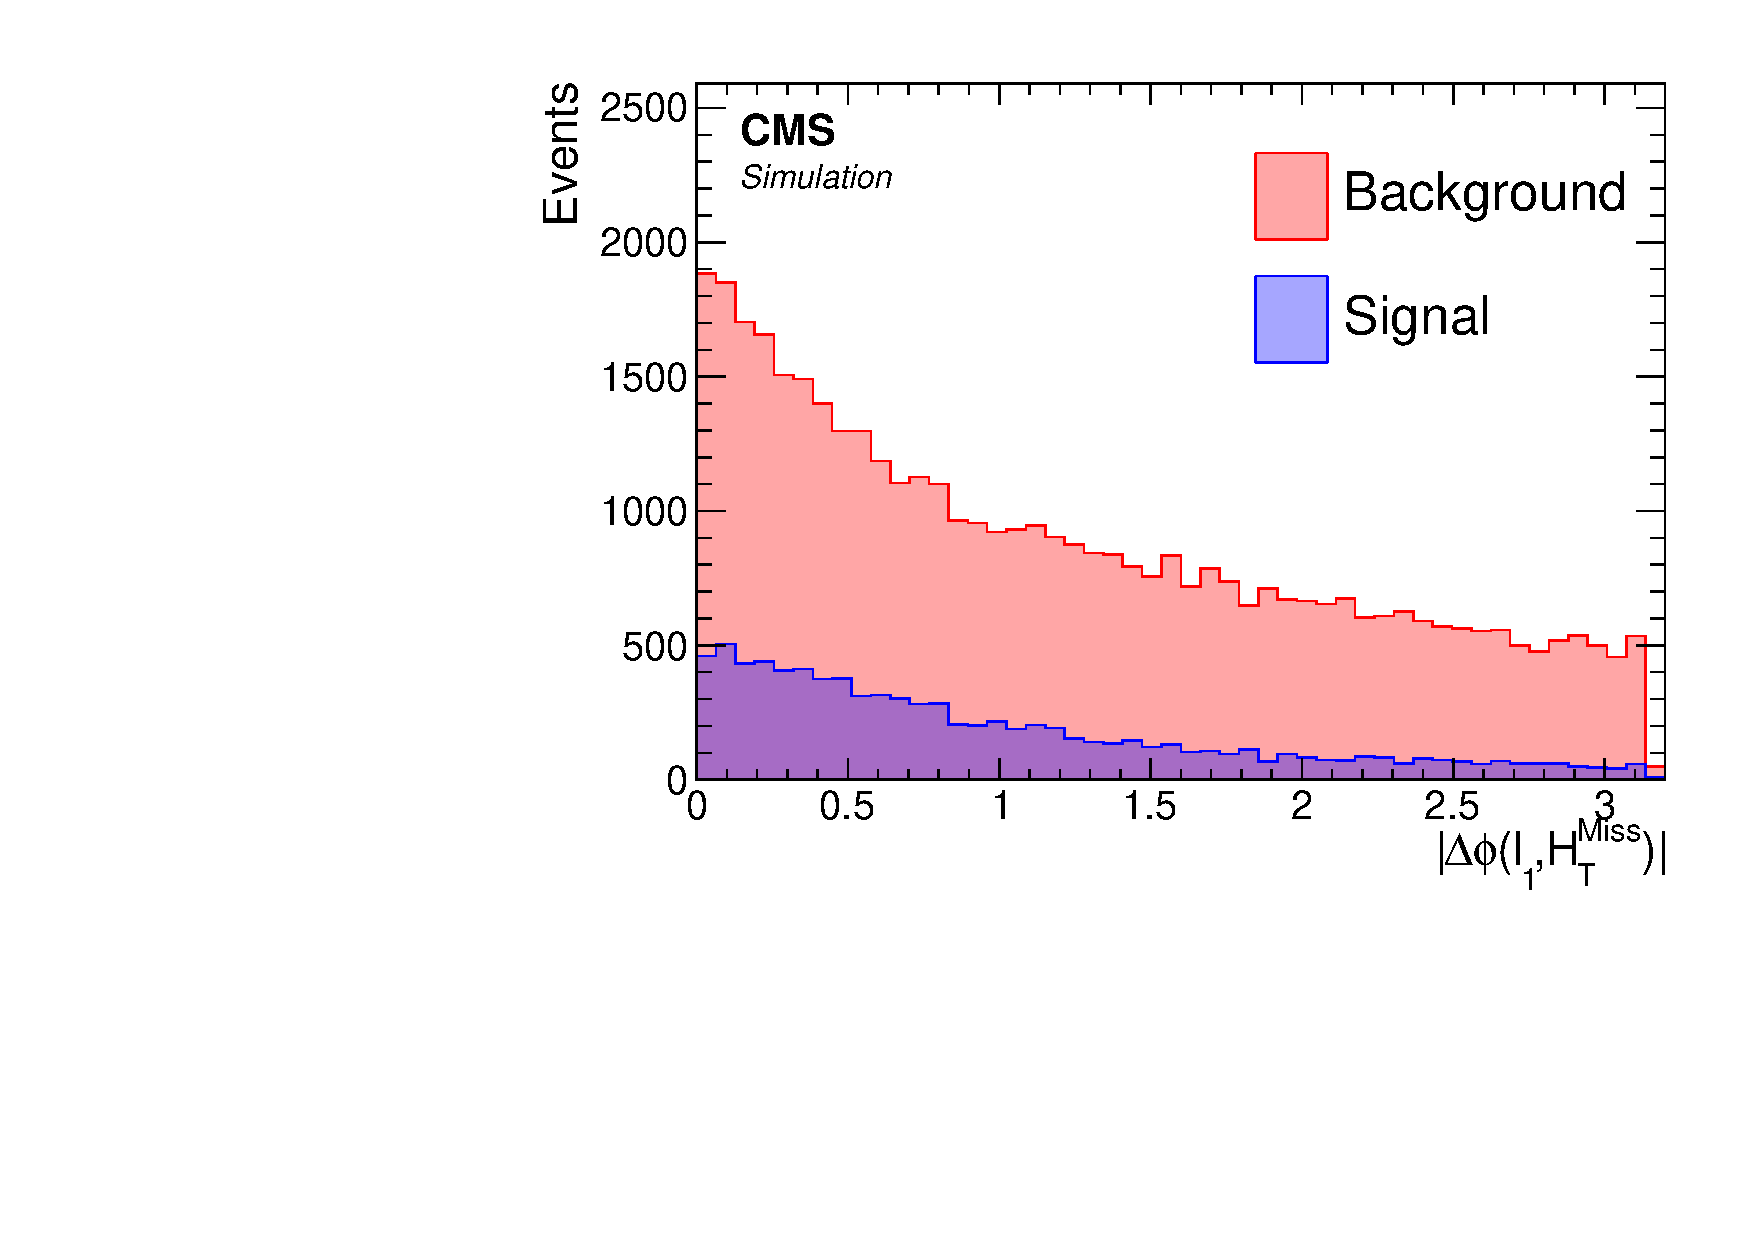
\includegraphics[width=0.32\linewidth]{plots/dilepton_bdt_inputs_muons/none_deltaPhiMhtLepton1CorrJetNoMultIso10Dr0.6.pdf} \,
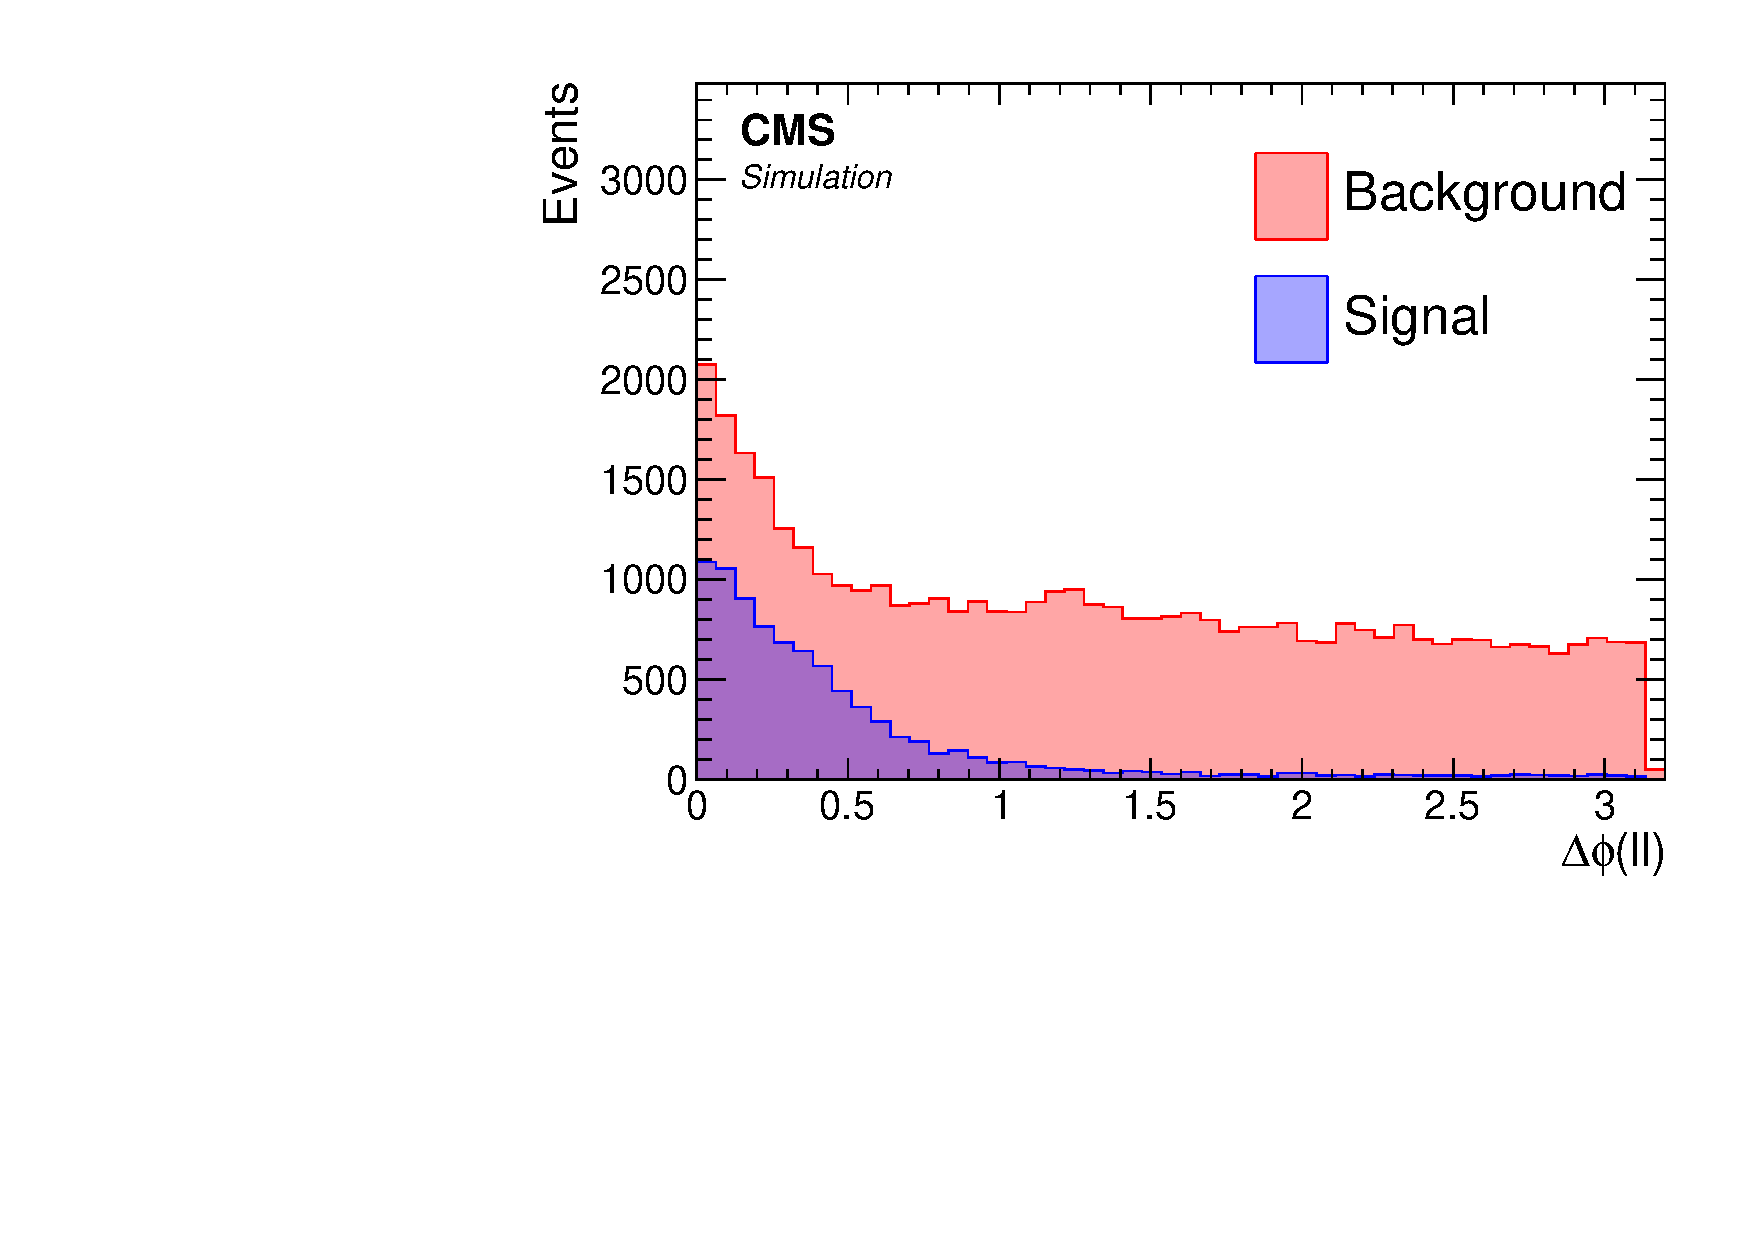
\includegraphics[width=0.32\linewidth]{plots/dilepton_bdt_inputs_muons/none_deltaPhiCorrJetNoMultIso10Dr0.6.pdf} \,
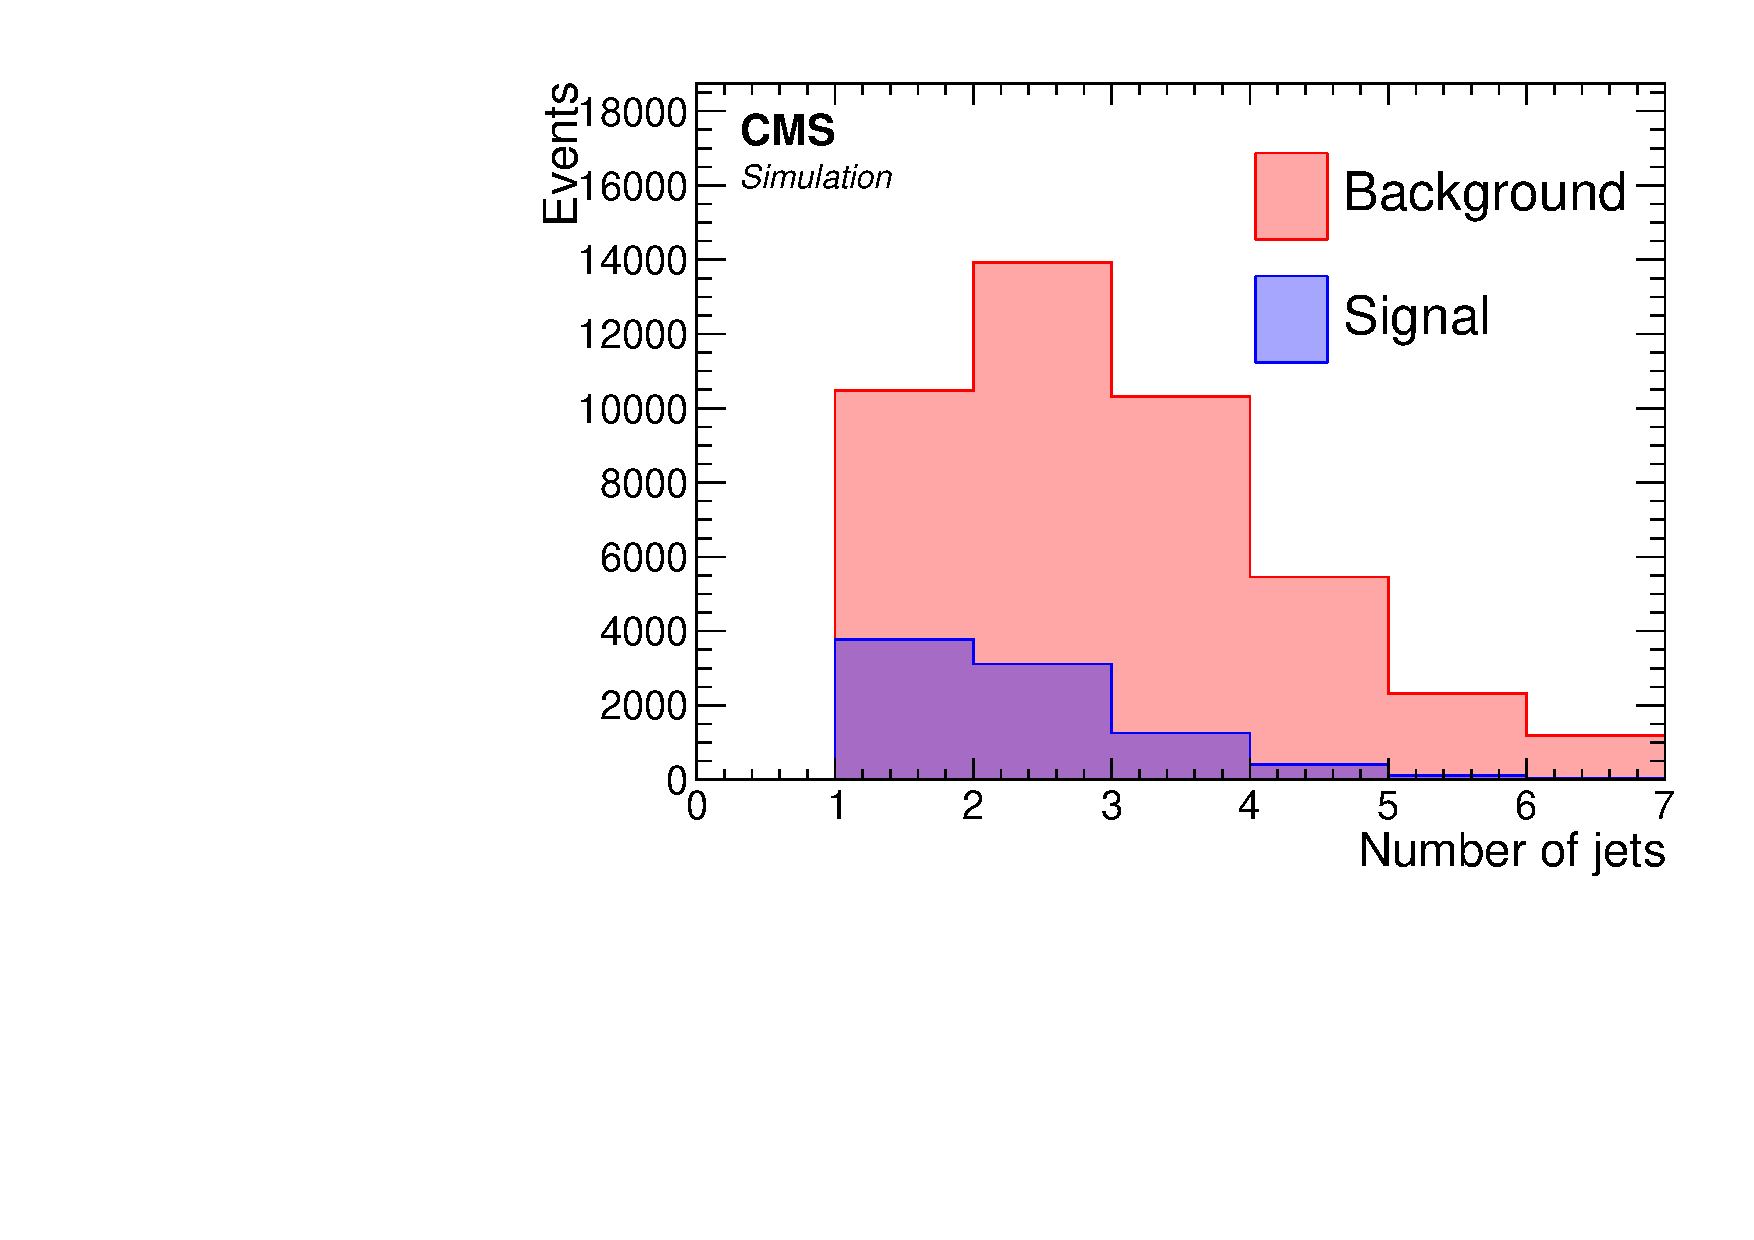
\includegraphics[width=0.32\linewidth]{plots/dilepton_bdt_inputs_muons/none_NJets.pdf}   \\
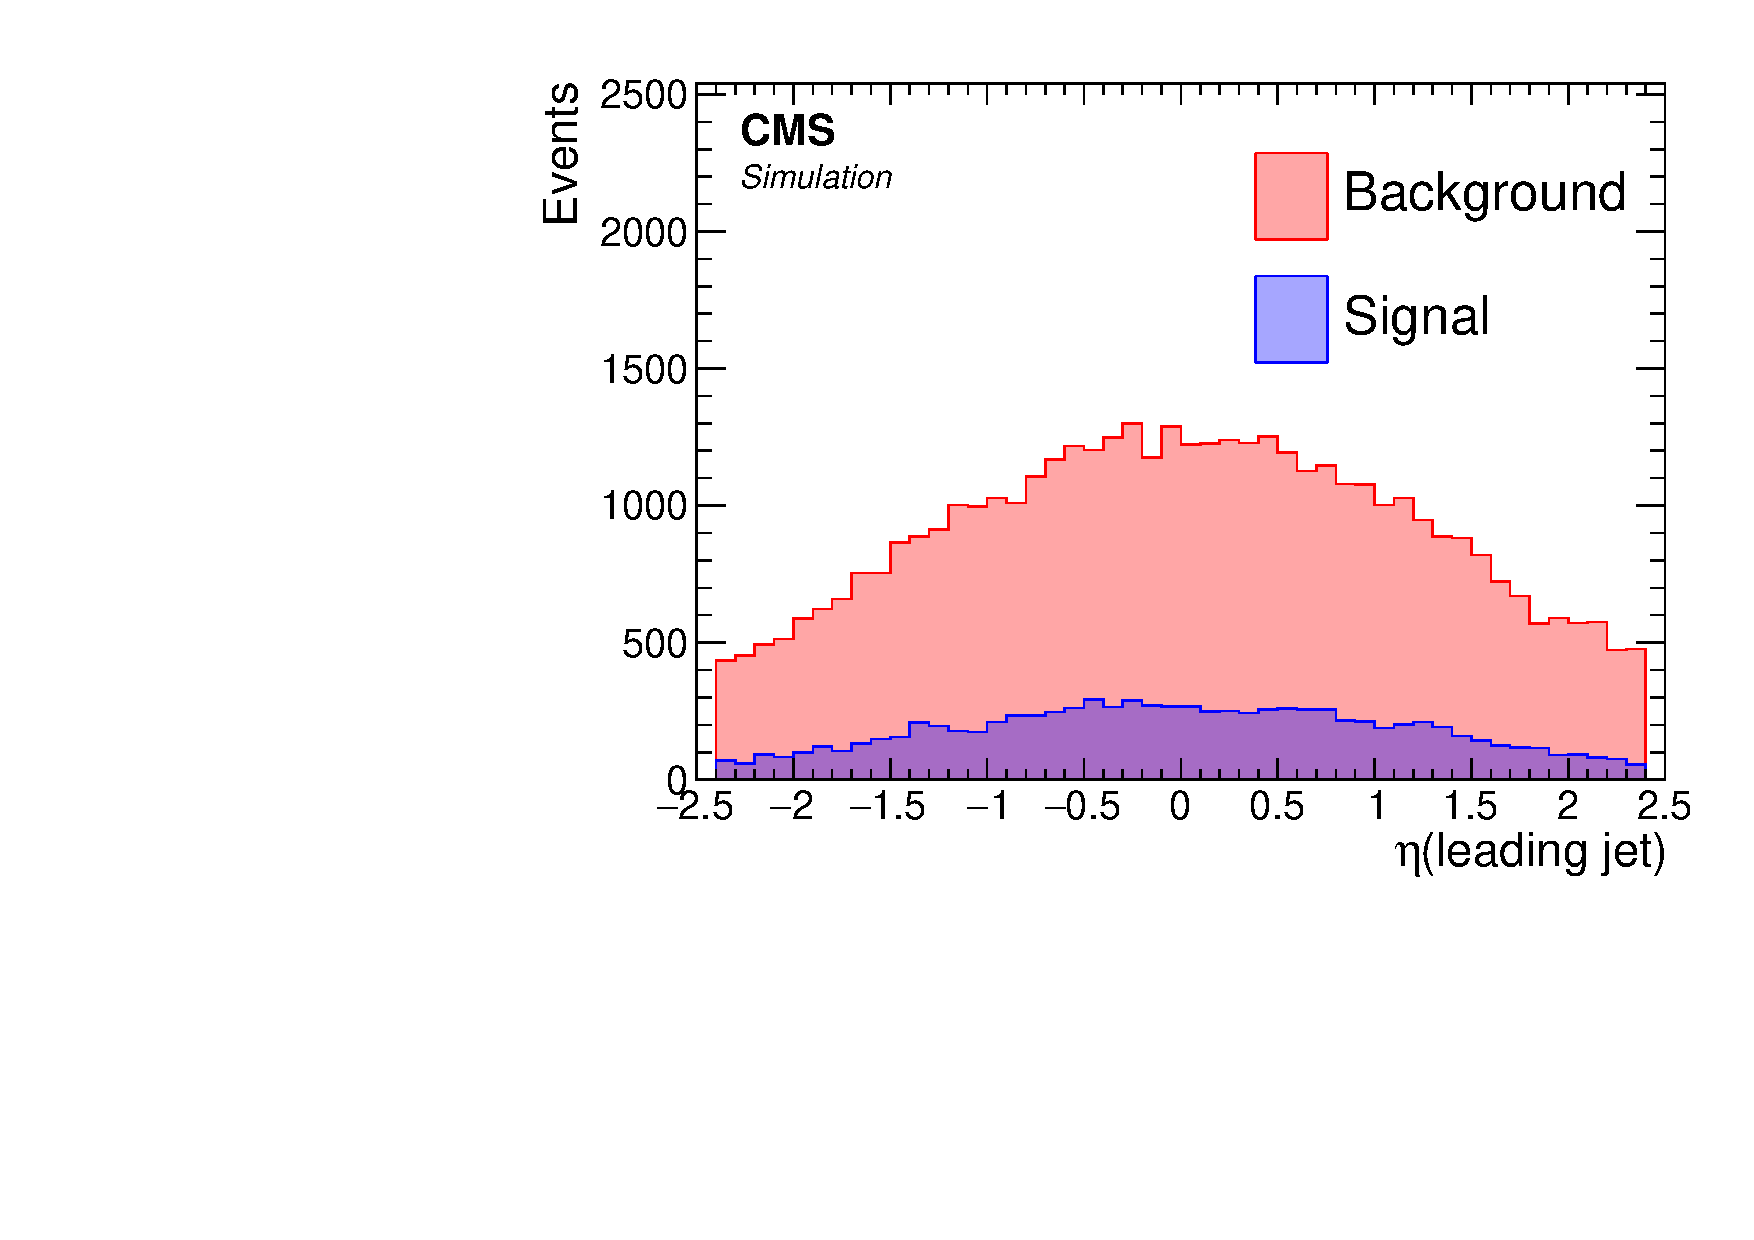
\includegraphics[width=0.32\linewidth]{plots/dilepton_bdt_inputs_muons/none_LeadingJet.Eta__.pdf} \,
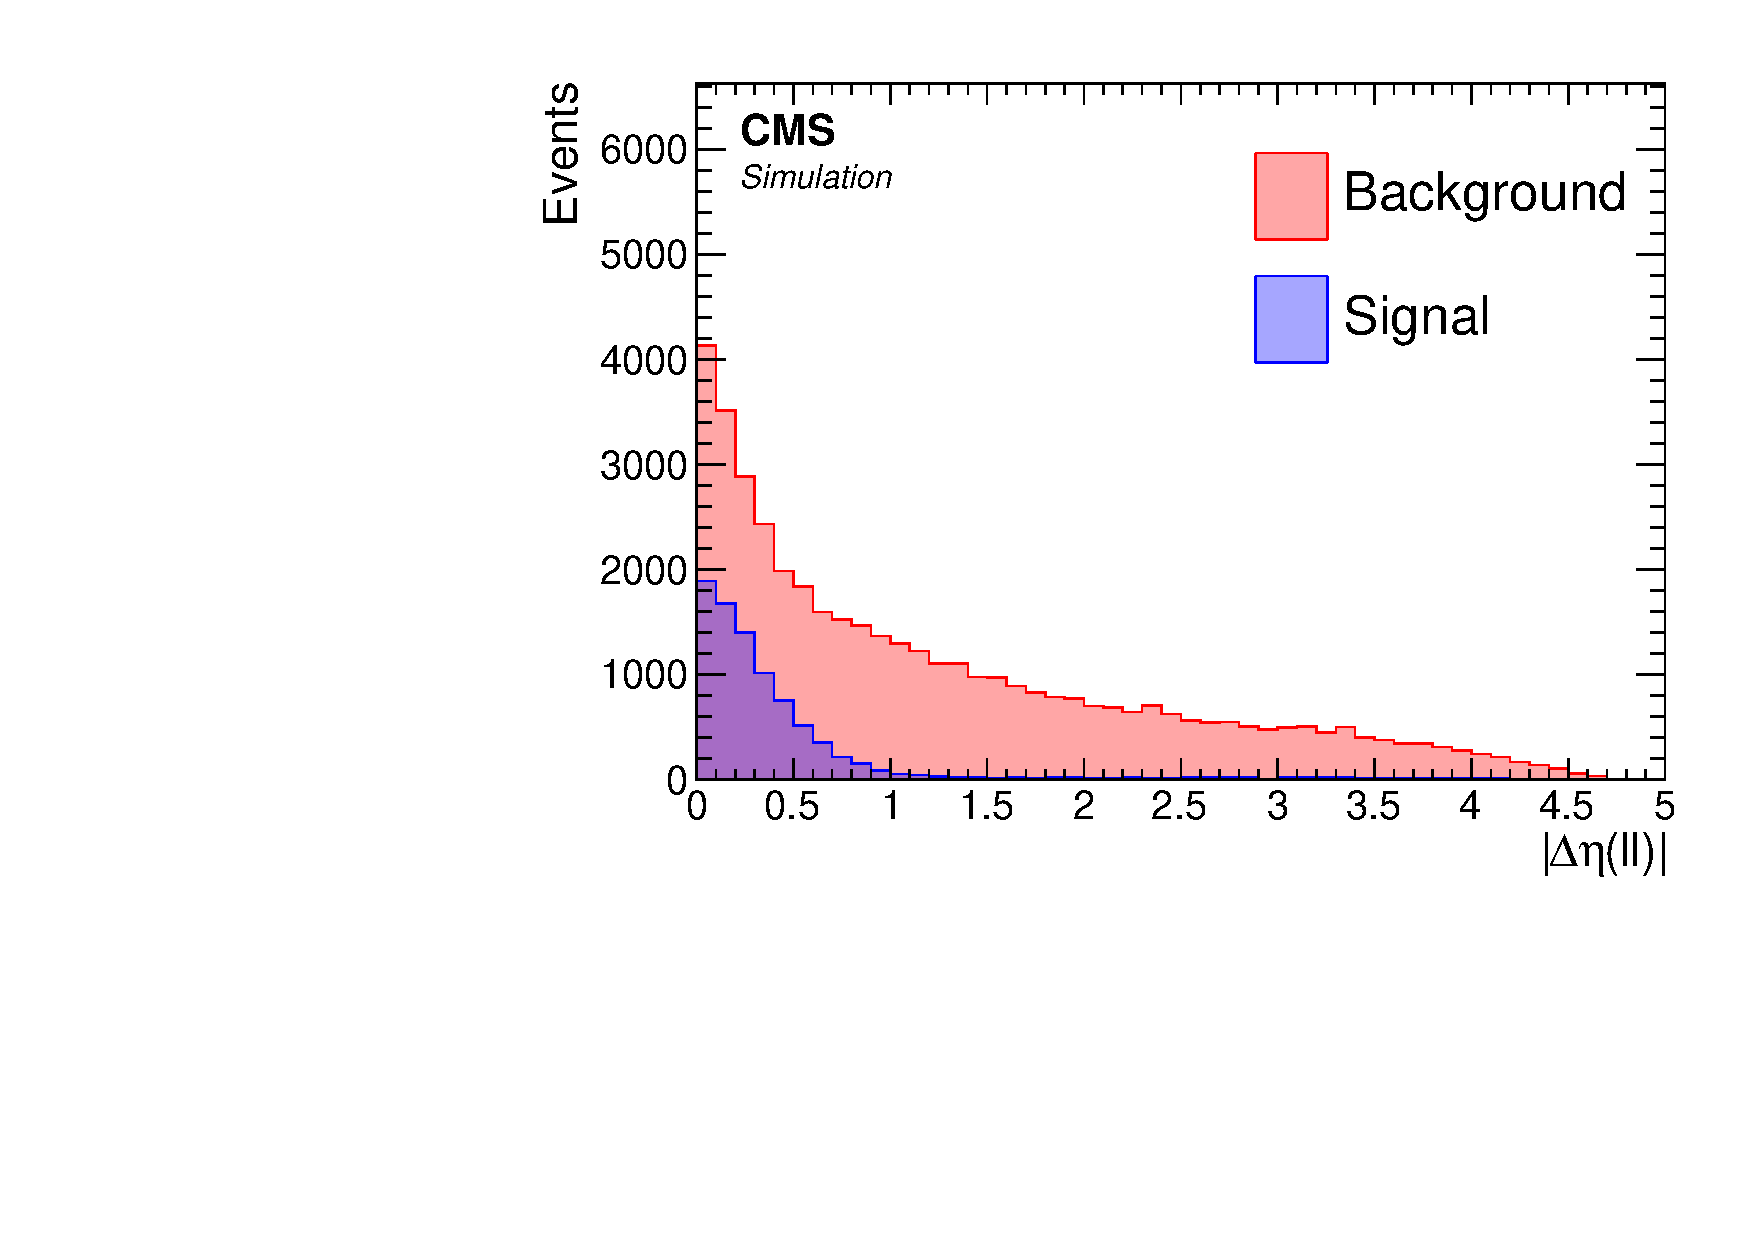
\includegraphics[width=0.32\linewidth]{plots/dilepton_bdt_inputs_muons/none_deltaEtaCorrJetNoMultIso10Dr0.6.pdf}  \,
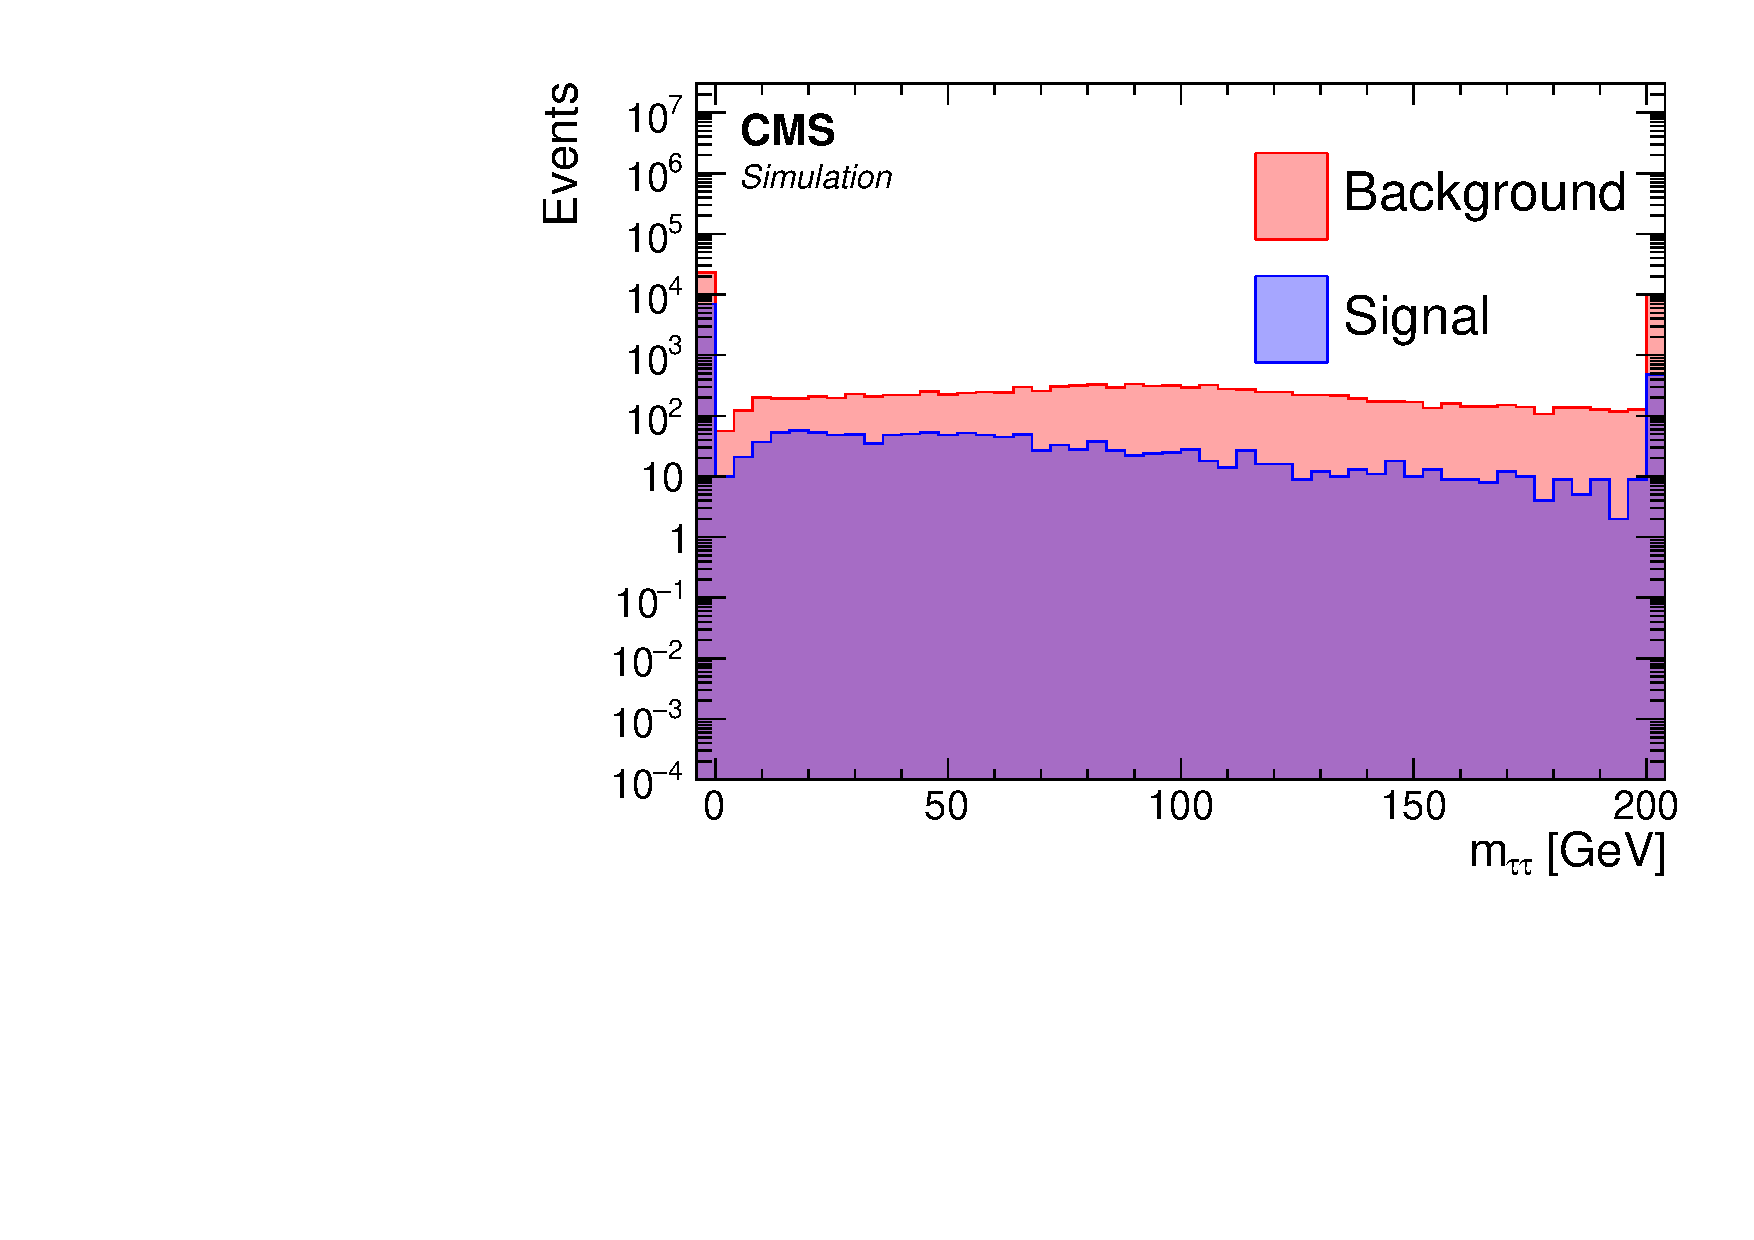
\includegraphics[width=0.32\linewidth]{plots/dilepton_bdt_inputs_muons/none_nmtautauCorrJetNoMultIso10Dr0.6_log.pdf} \\

\caption[dimuon training input distribution]{Dimuon BDT training input variables. Ordered by importance ranking.}
\label{fig:dimuon-input-distributions}
\end{figure}

\clearpage
\subsubsection{Exclusive track category}

The training samples in phase 0 for the exclusive  category contain 7863 (1750) signal events and 55765 (29135) background events for muons (electrons) flavor. For phase 1,  the exclusive  category contain 5266 (1332) signal events and 51308 (31149) background events for muons (electrons) flavor. The training samples are then tested against the test samples of equal size. The distributions of the testing samples overlay on the training samples are seen in~\ref{fig:event-bdt-ex-track-output}. No significant over training is observed. The ROC curves are seen in~\ref{fig:event-bdt-ex-track-roc}.

\begin{figure}[!htb]
\centering
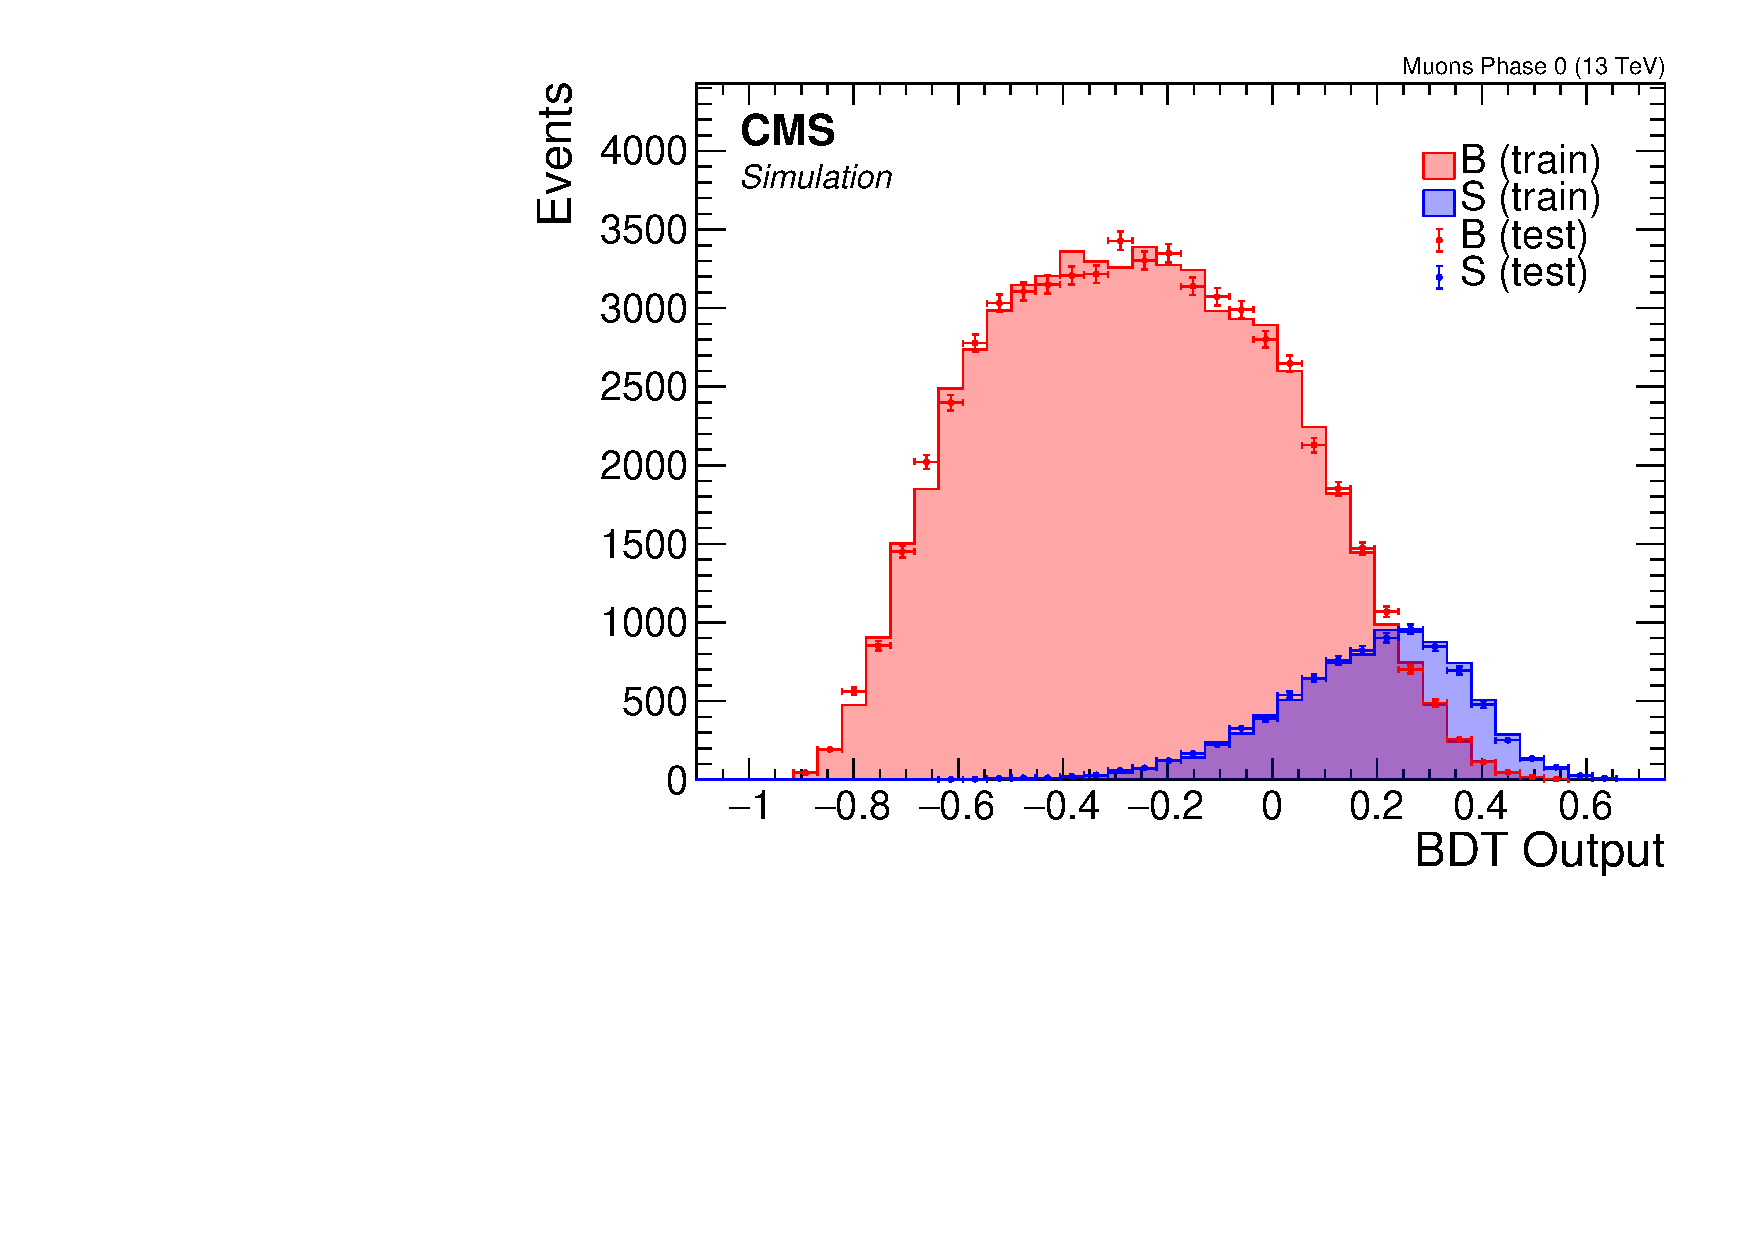
\includegraphics[width=0.48\linewidth]{plots/extrack_bdt/overtraining_Event_Ex_Track_Muons_Phase_0.pdf} \,
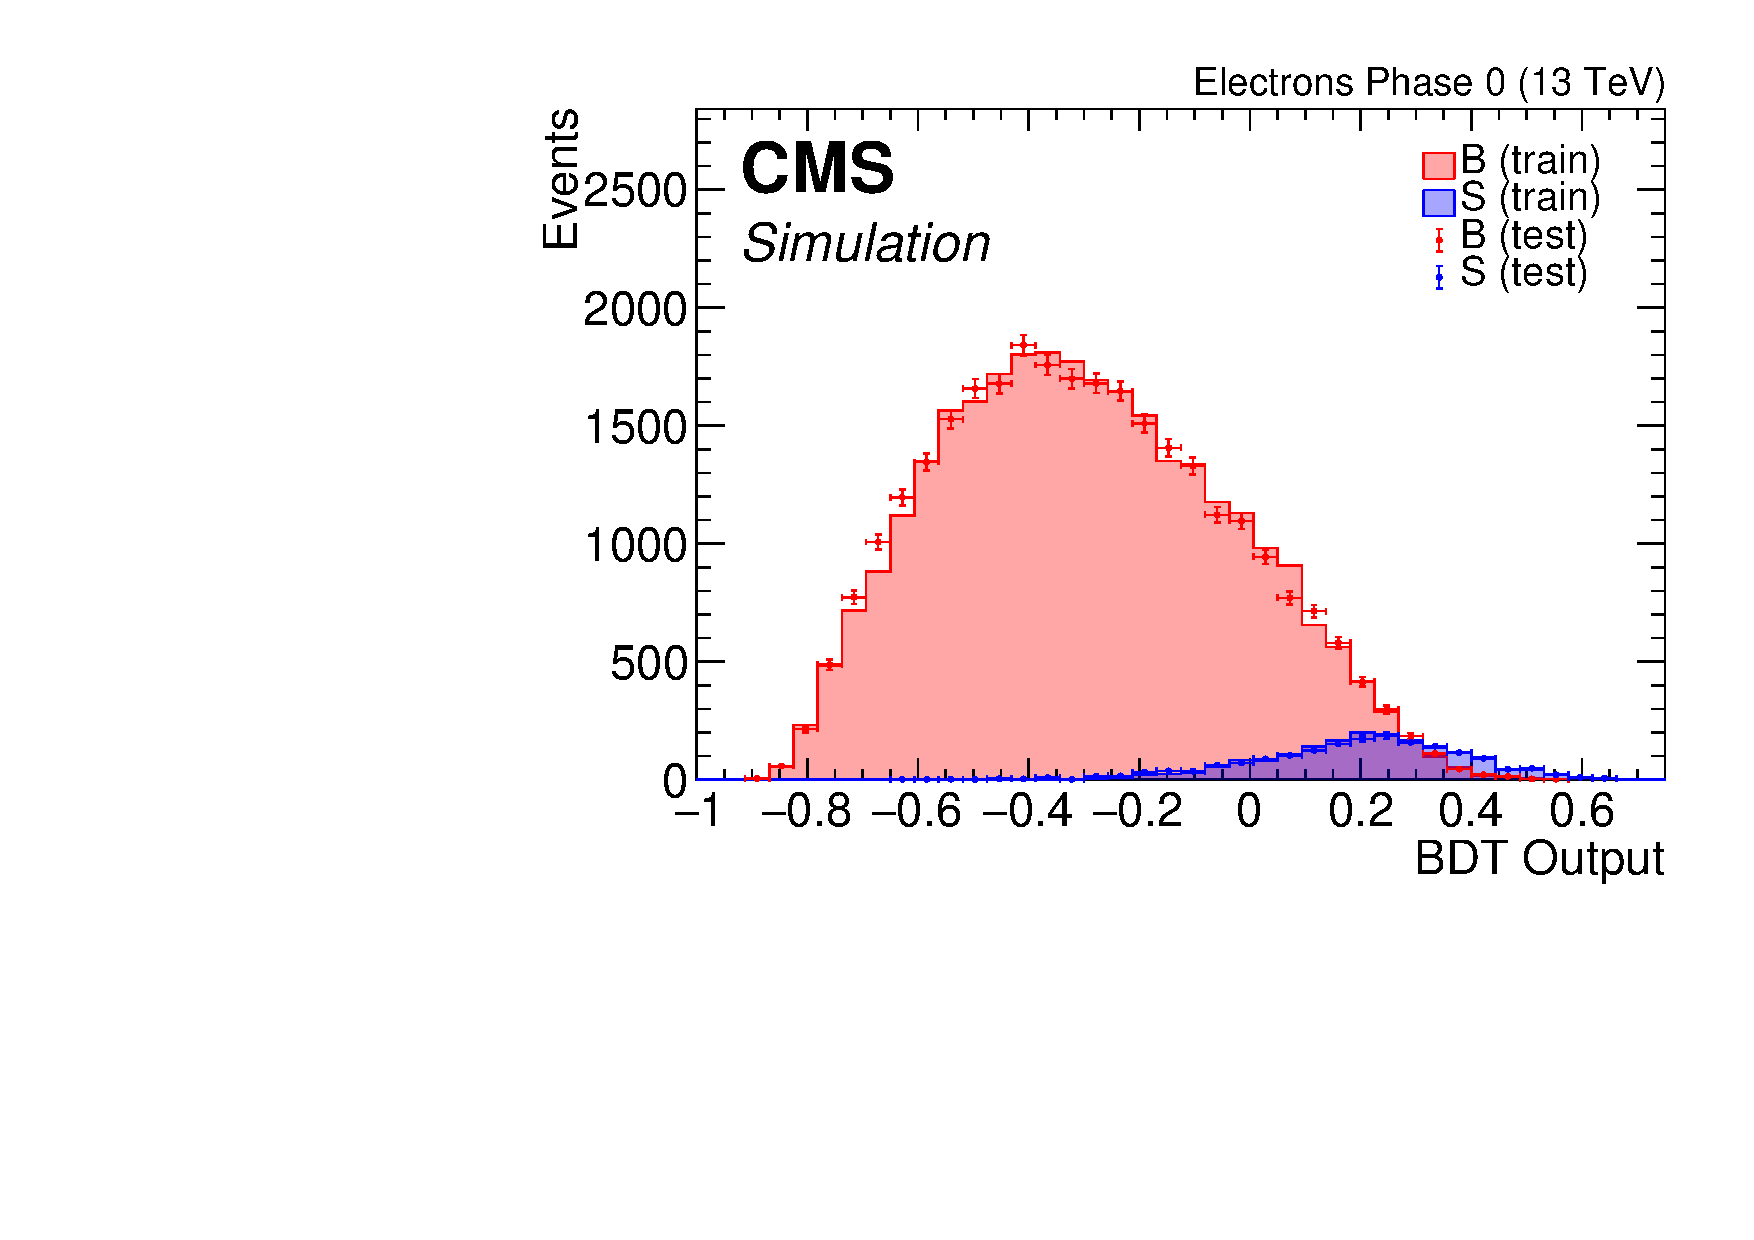
\includegraphics[width=0.48\linewidth]{plots/extrack_bdt/overtraining_Event_Ex_Track_Electrons_Phase_0.pdf} \\

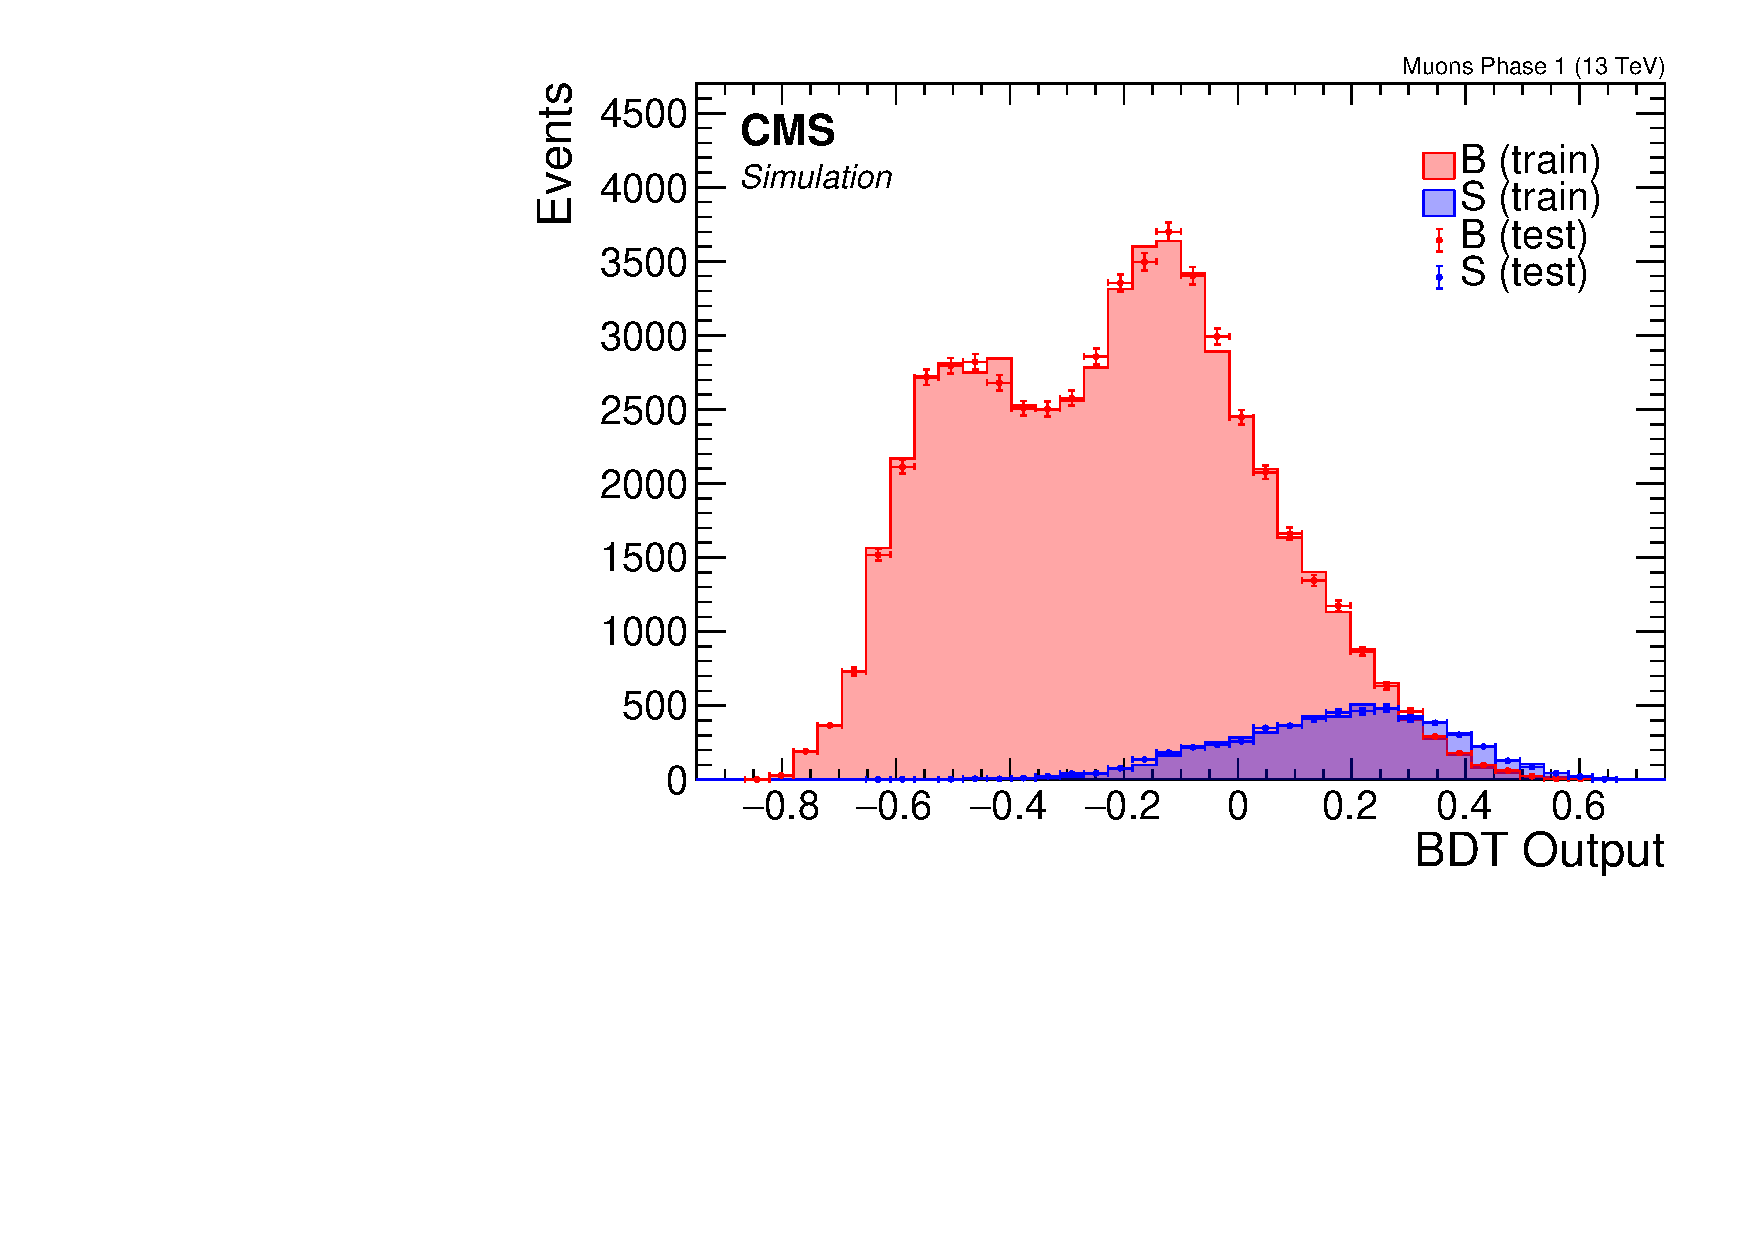
\includegraphics[width=0.48\linewidth]{plots/extrack_bdt/overtraining_Event_Ex_Track_Muons_Phase_1.pdf} \,
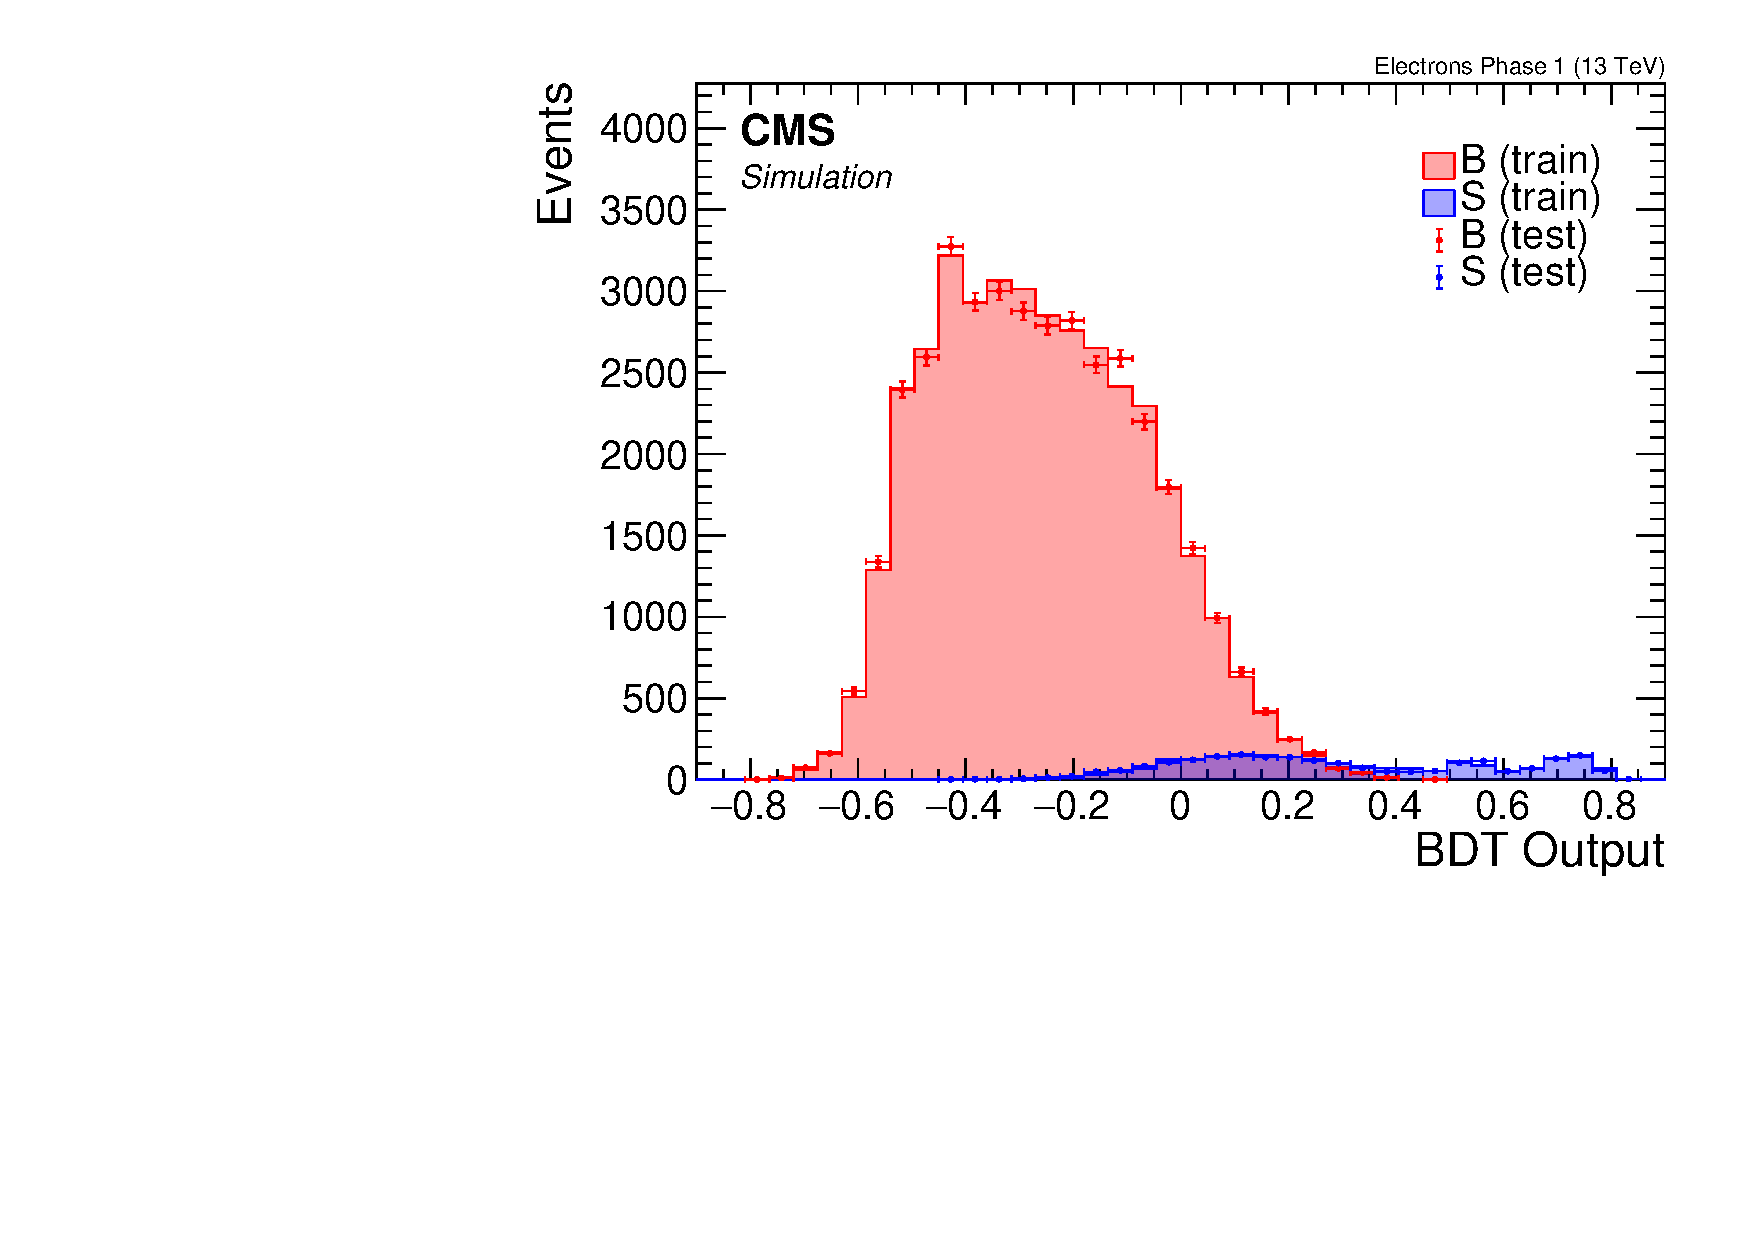
\includegraphics[width=0.48\linewidth]{plots/extrack_bdt/overtraining_Event_Ex_Track_Electrons_Phase_1.pdf} \\

\caption[Exclusive track category BDT outputs]{Exclusive track category BDT output in phase 0 (top) and phase 1 (bottom) for muons (left) and electrons (right)}
\label{fig:event-bdt-ex-track-output}
\end{figure}

\begin{figure}[!htb]
\centering
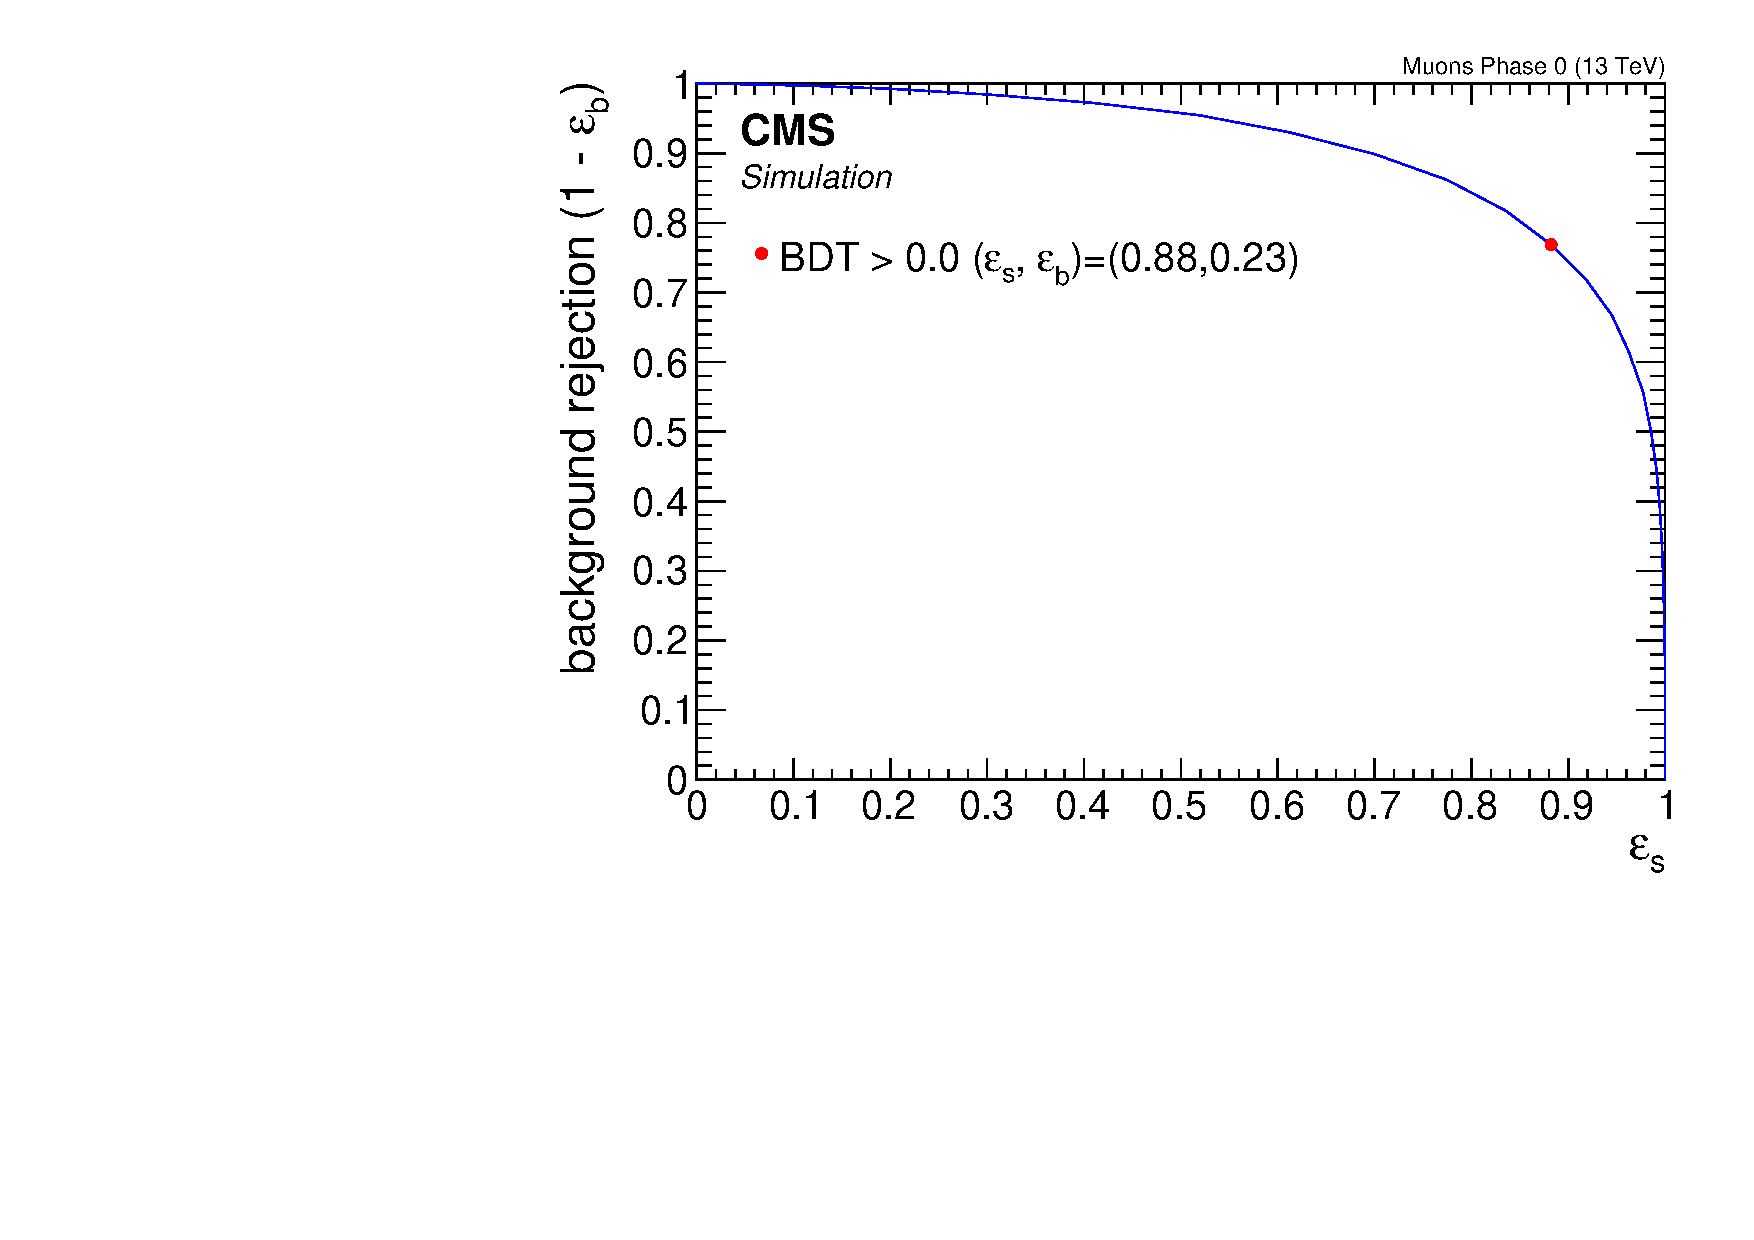
\includegraphics[width=0.48\linewidth]{plots/extrack_bdt/roc_Event_Ex_Track_Muons_Phase_0.pdf} \,
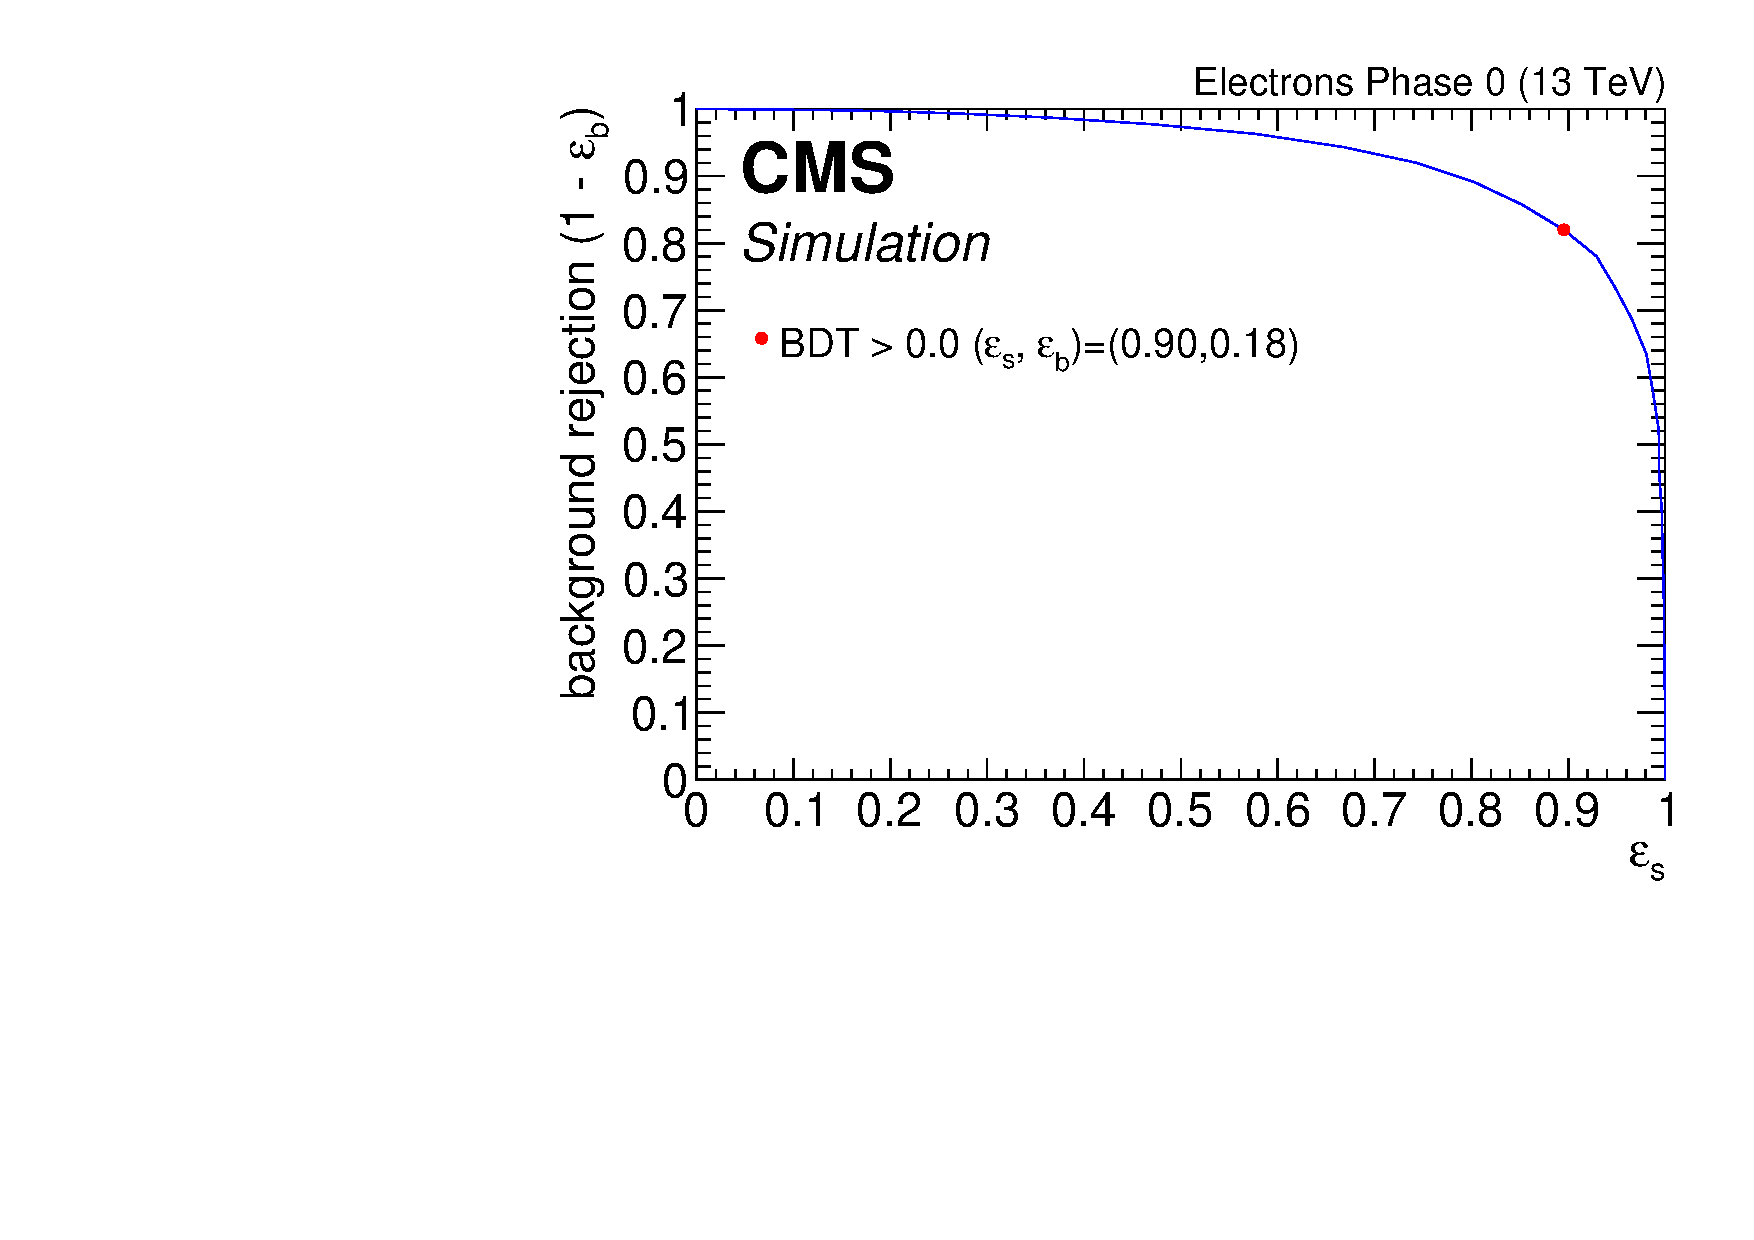
\includegraphics[width=0.48\linewidth]{plots/extrack_bdt/roc_Event_Ex_Track_Electrons_Phase_0.pdf} \\

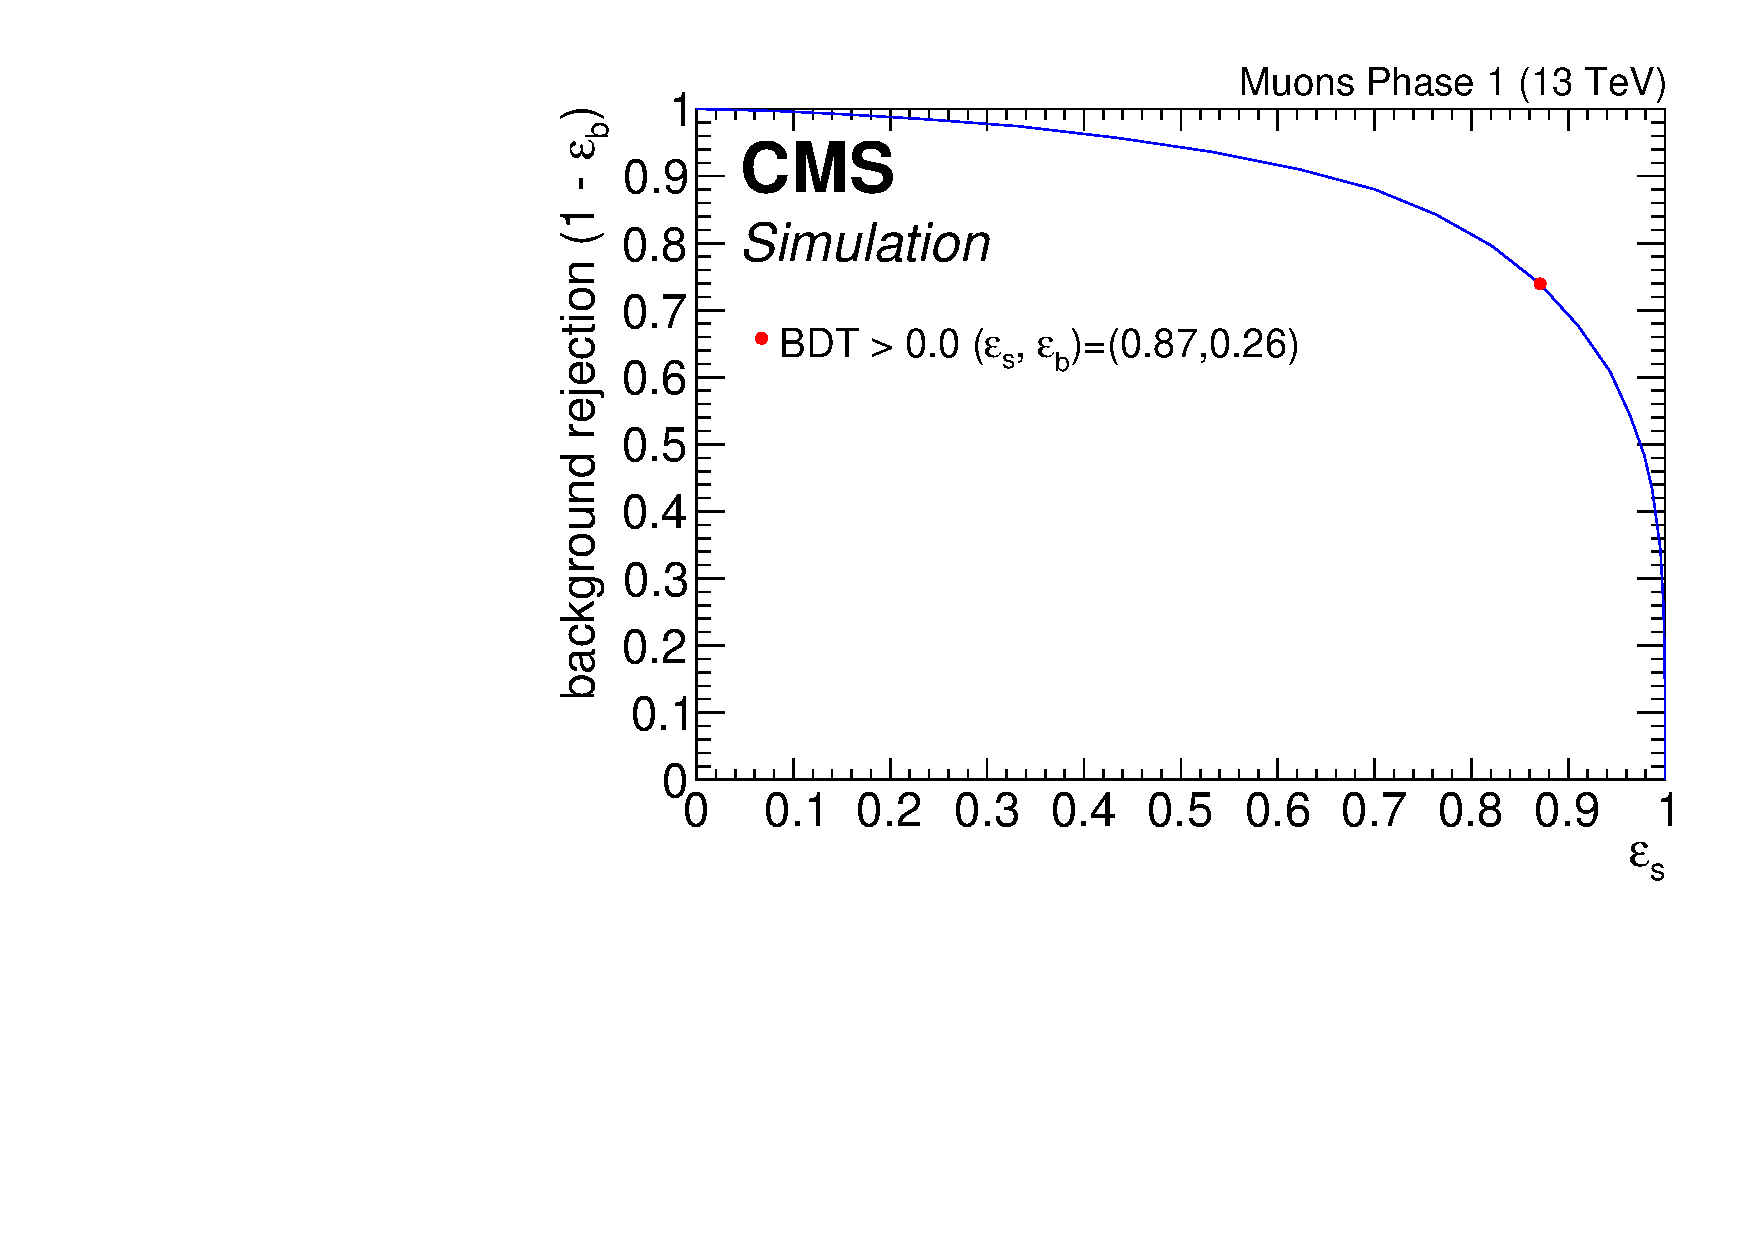
\includegraphics[width=0.48\linewidth]{plots/extrack_bdt/roc_Event_Ex_Track_Muons_Phase_1.pdf} \,
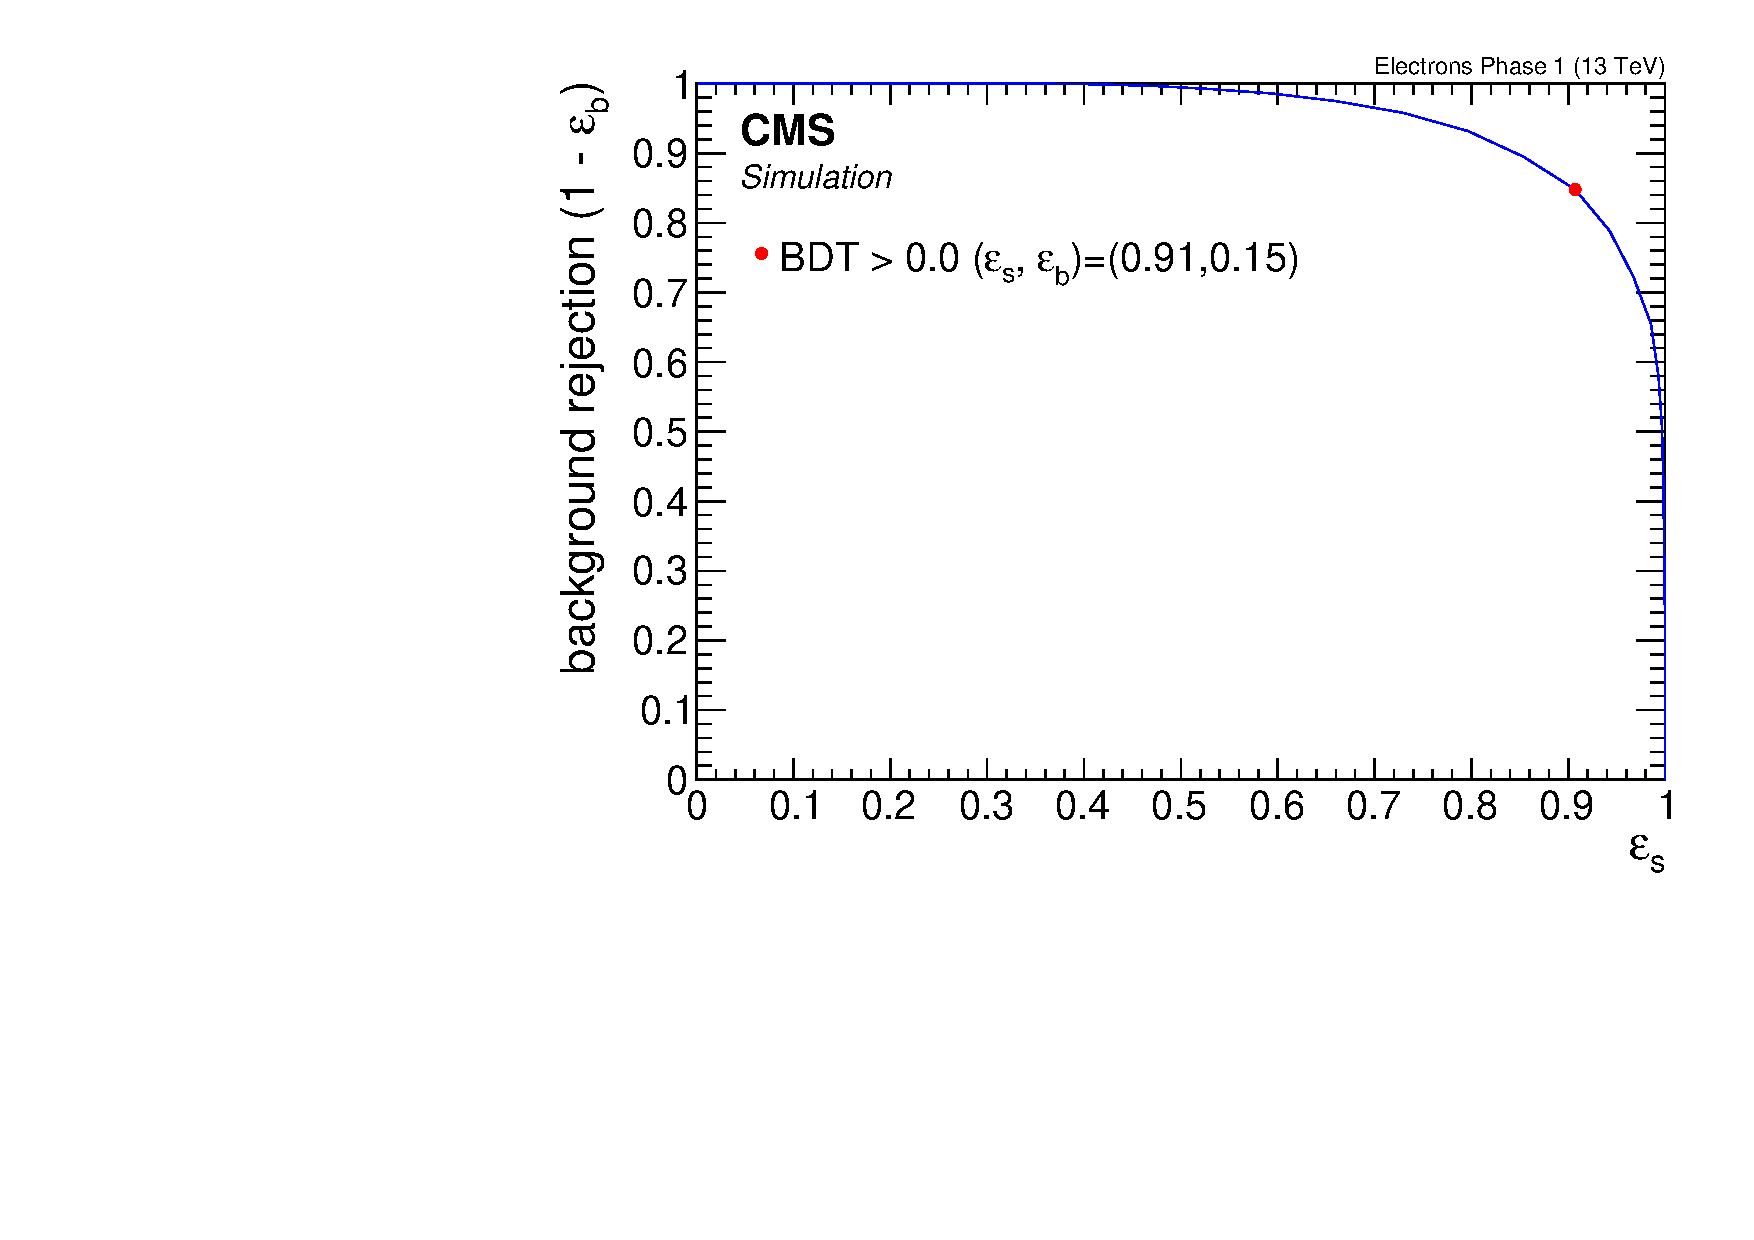
\includegraphics[width=0.48\linewidth]{plots/extrack_bdt/roc_Event_Ex_Track_Electrons_Phase_1.pdf} \\

\caption[Exclusive track category ROC curve]{Exclusive track category ROC curves in phase 0 (top) and phase 1 (bottom) for muons (left) and electrons (right)}
\label{fig:event-bdt-ex-track-roc}
\end{figure}

The training uses 18 different variables listed in Table~\ref{tab:extrack-bdt-variables} in decreasing order of importance ranking. Since the ranking is slightly different in the four trainings, we choose here to list the order in the case of the muons of phase 1. We denote the fully identified lepton as $\ell$ and the non-identified lepton track as $t$.

\begin{table}[!htb]
	\centering
	\label{tab:extrack-bdt-variables}
		\caption{Exclusive track BDT input variables}
		%\vspace{1mm}
			\begin{tabular}{cll} \hline
			Rank & Variable & Description \\ \hline
			1 & $\pt(\ell)$ & lepton \pt\\
			2 & \HT & \\
			3 & \mht & \\
			4 & $\mindphimhtjets$ & \\
			5 & $\pt(\text{leading jet})$ & \\
			6 & $\njets$ & Number of jets \\					7 & track BDT output & \\
			8 & $\eta(t)$ & \\
			9 & $\pt(t)$ & track \pt\\
			10 & $\eta(\text{leading jet})$ & \\				11 & $\mll$ & invariant mass \\
			12 & $\eta(\ell)$ & \\
			13 & $m_T(\ell)$ & lepton transverse mass\\			
			14 & $\DR\left(\ell, t\right)$ & \\
			15 & $\phi(\ell)$ & \\
			16 & $\phi(t)$ & \\
			17 & $\abs{\Delta\phi\left(\ell,t \right)}$ & \\			
			18 & $\abs{\Delta \eta \left(\ell, t\right) }$ & \\			
			\hline
			\end{tabular}
\end{table}

Distributions of the input variables to the \gls{bdt} training can be seen in~\ref{fig:extrack-input-distributions}. As mentioned before, the signal is taken from a pool of a range of model points, and events are not weighted to any luminosity or cross section in order to avoid over training. In the following sections we will look at fully weighted distributions in order to asses the performance of the training for different model points and to understand the different components of the standard model background and how to estimate it properly.

\begin{figure}[!htb]
\centering
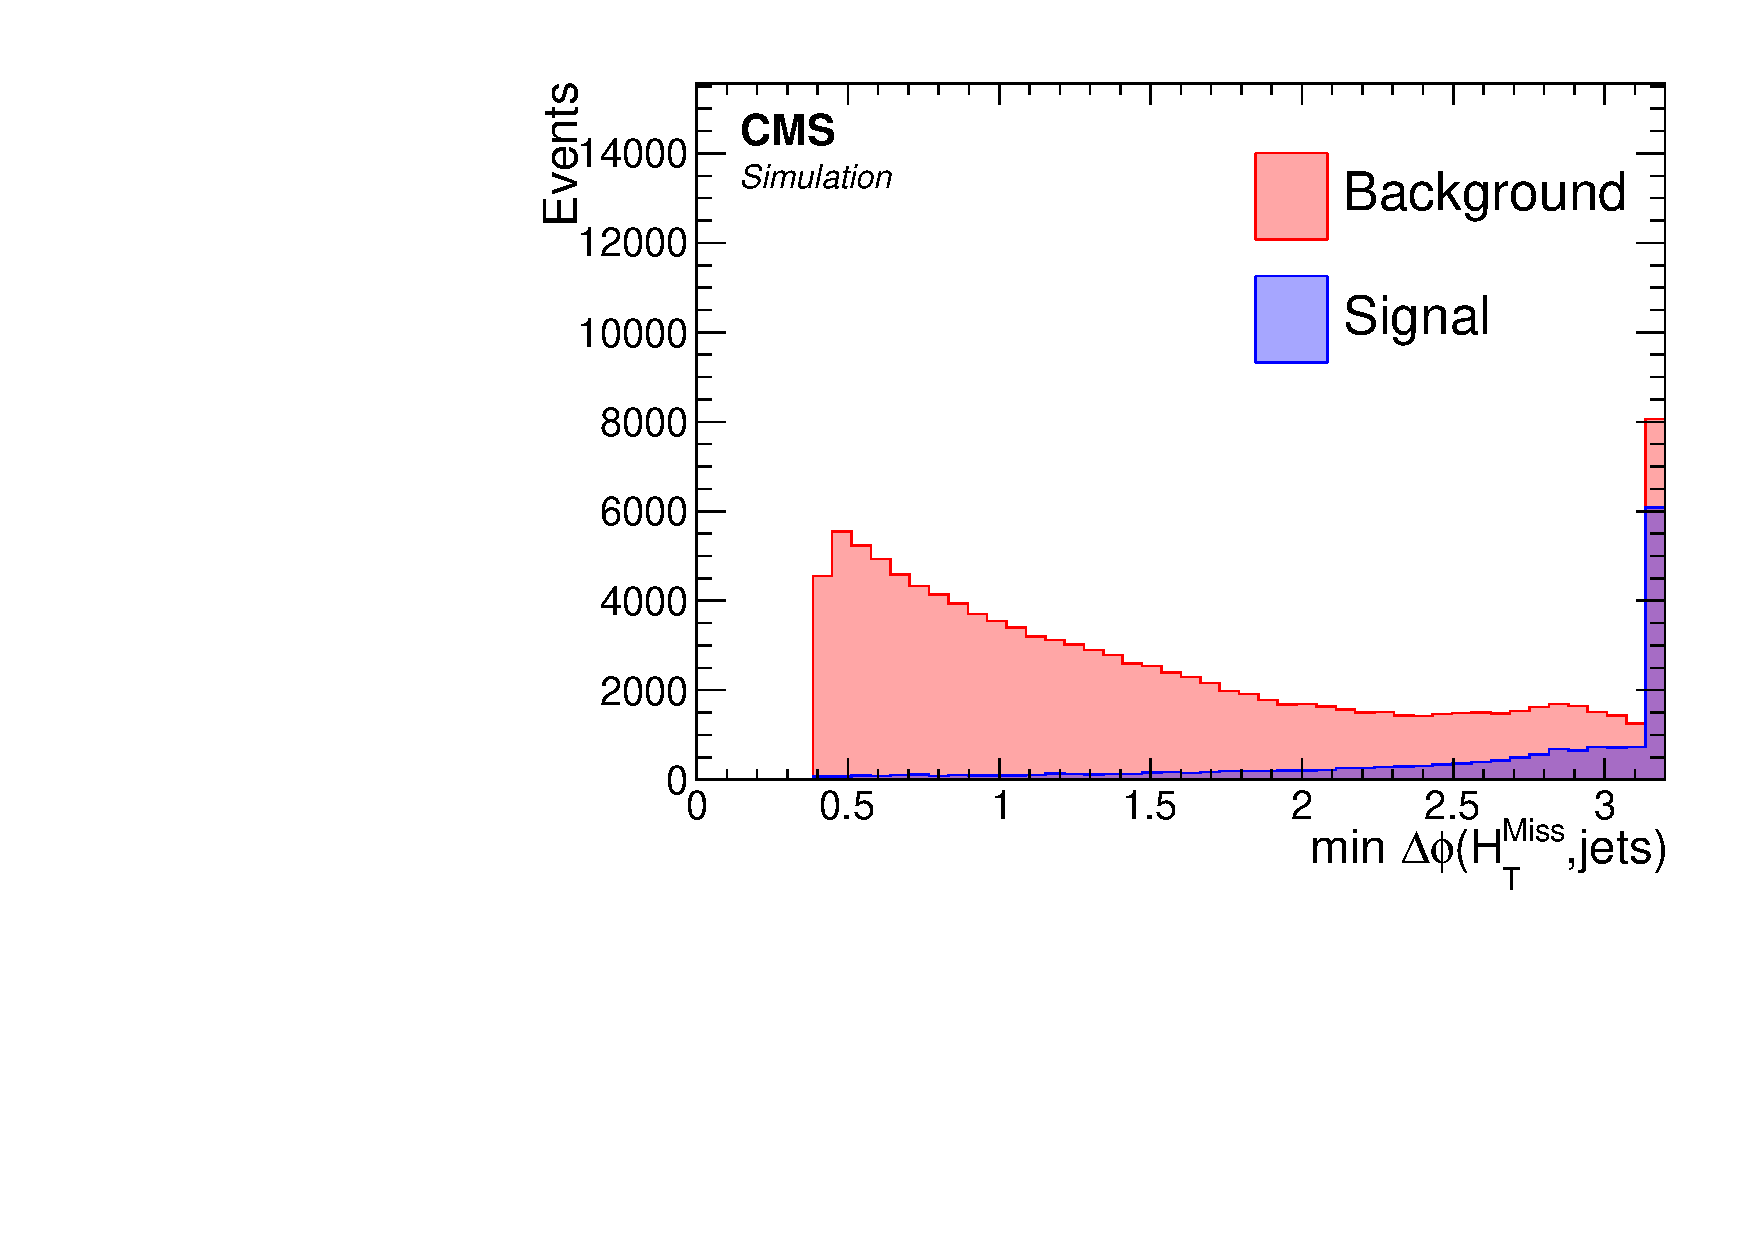
\includegraphics[width=0.32\linewidth]{plots/extrack_bdt_inputs_muons/none_MinDeltaPhiMhtJets.pdf} \,
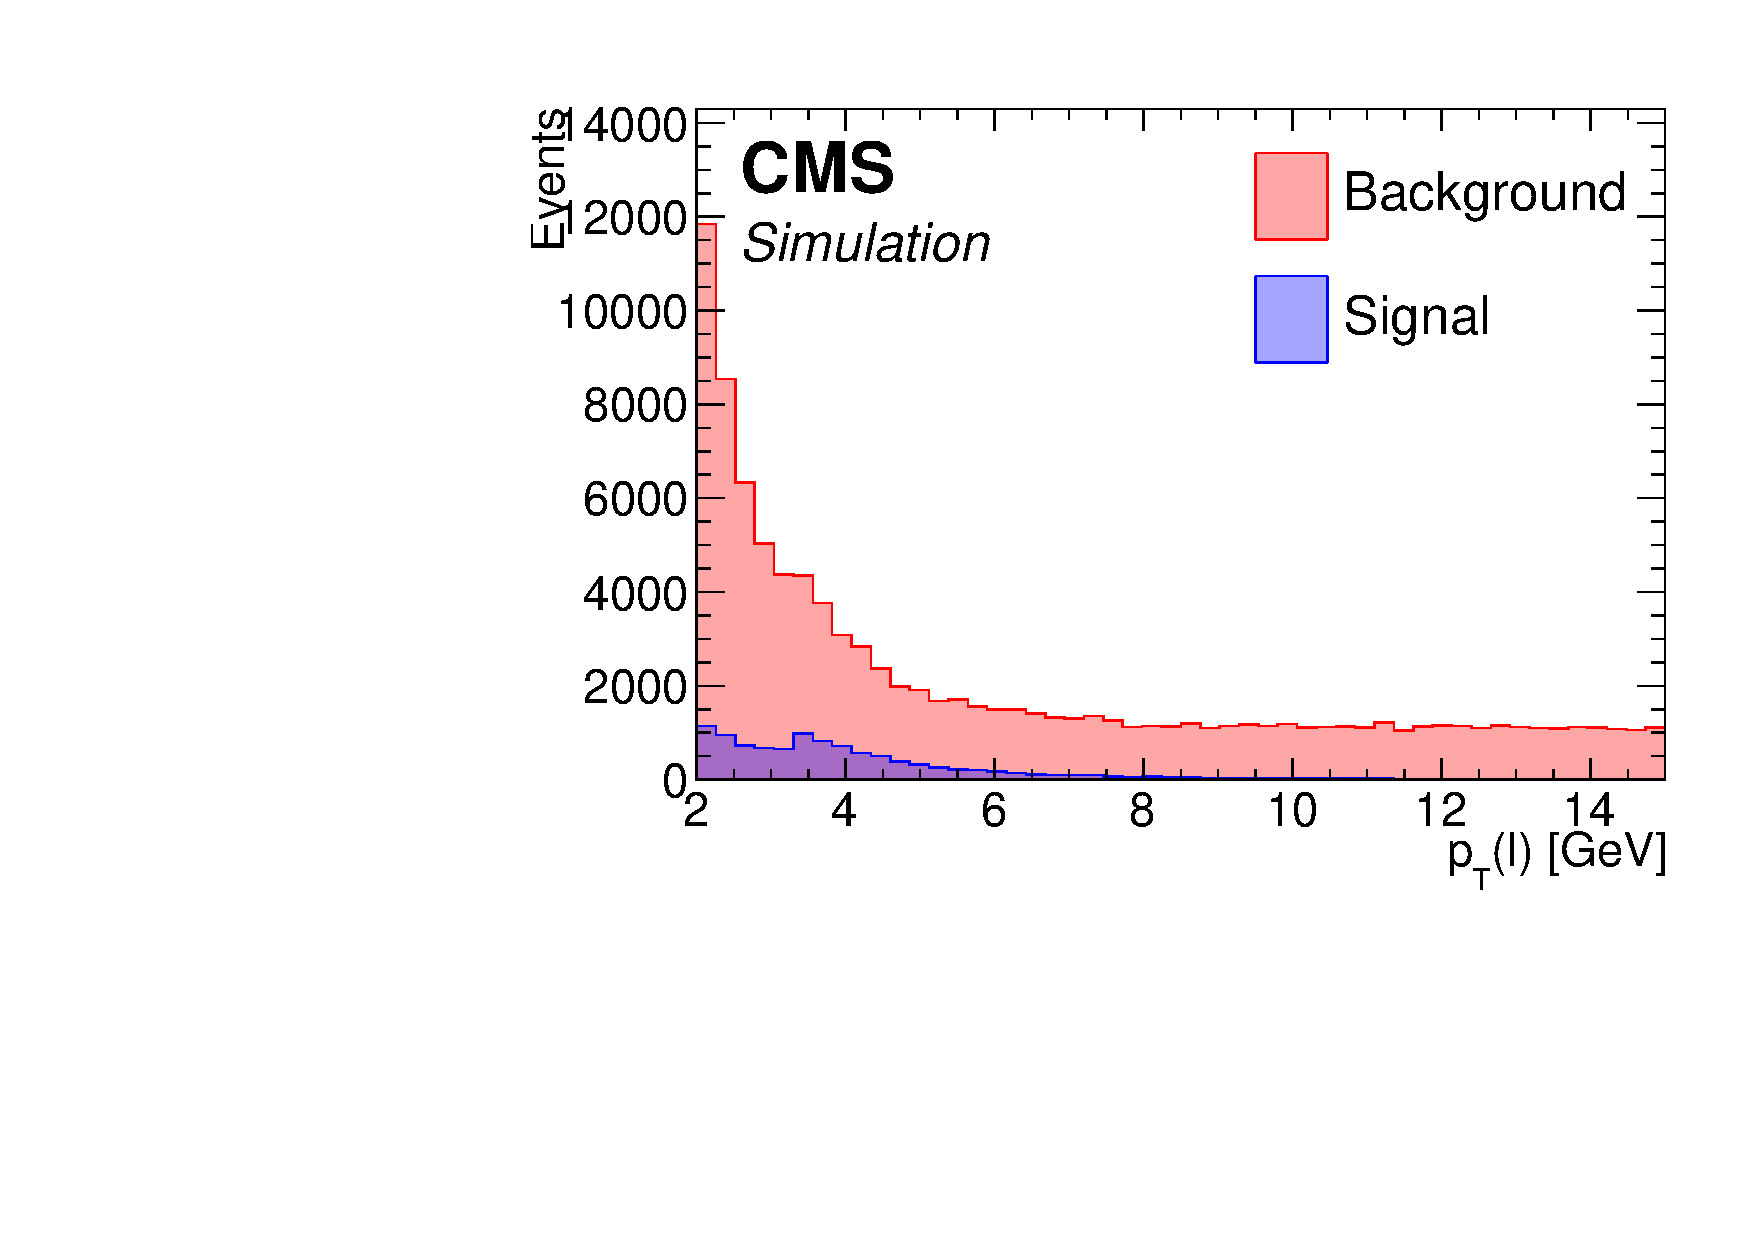
\includegraphics[width=0.32\linewidth]{plots/extrack_bdt_inputs_muons/none_leptonCorrJetNoMultIso10Dr0.6.Pt__.pdf} \,
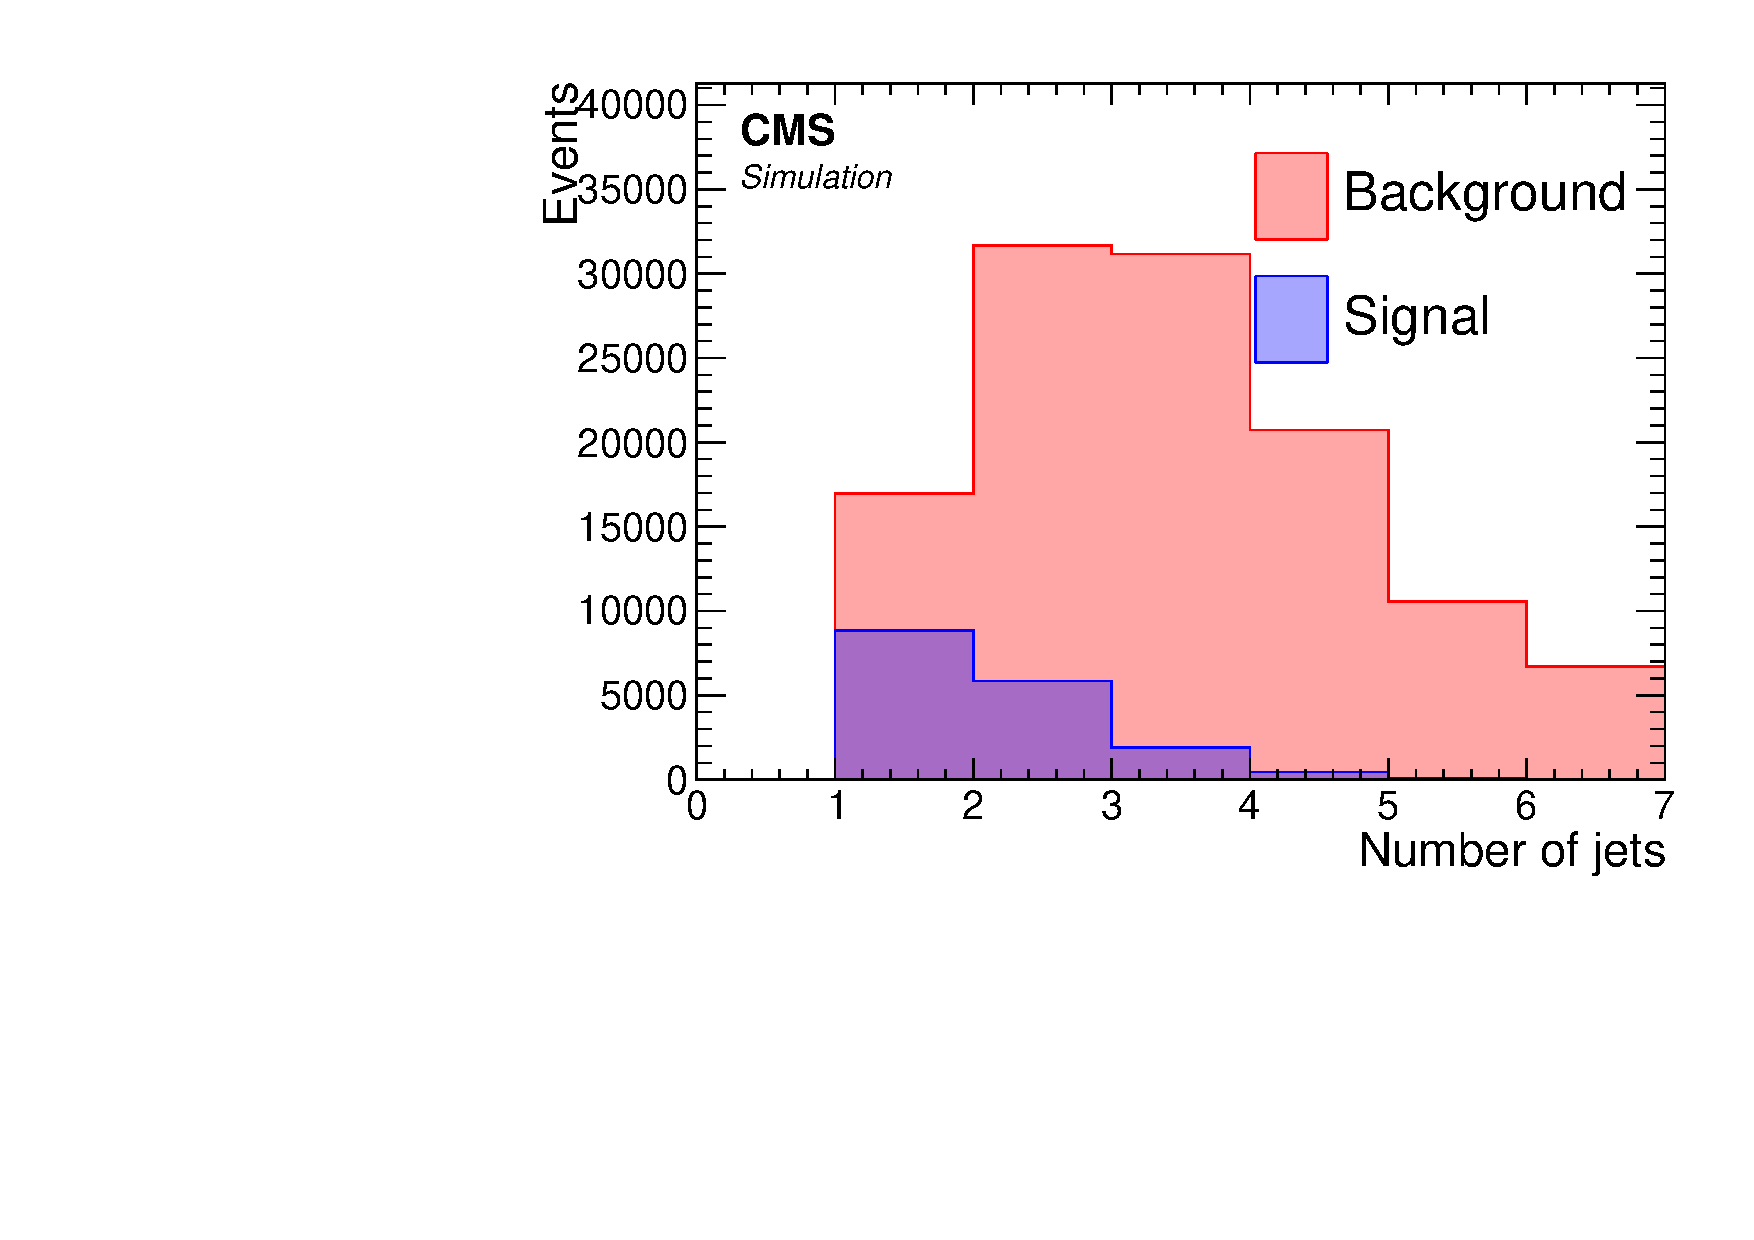
\includegraphics[width=0.32\linewidth]{plots/extrack_bdt_inputs_muons/none_NJets.pdf}   \\
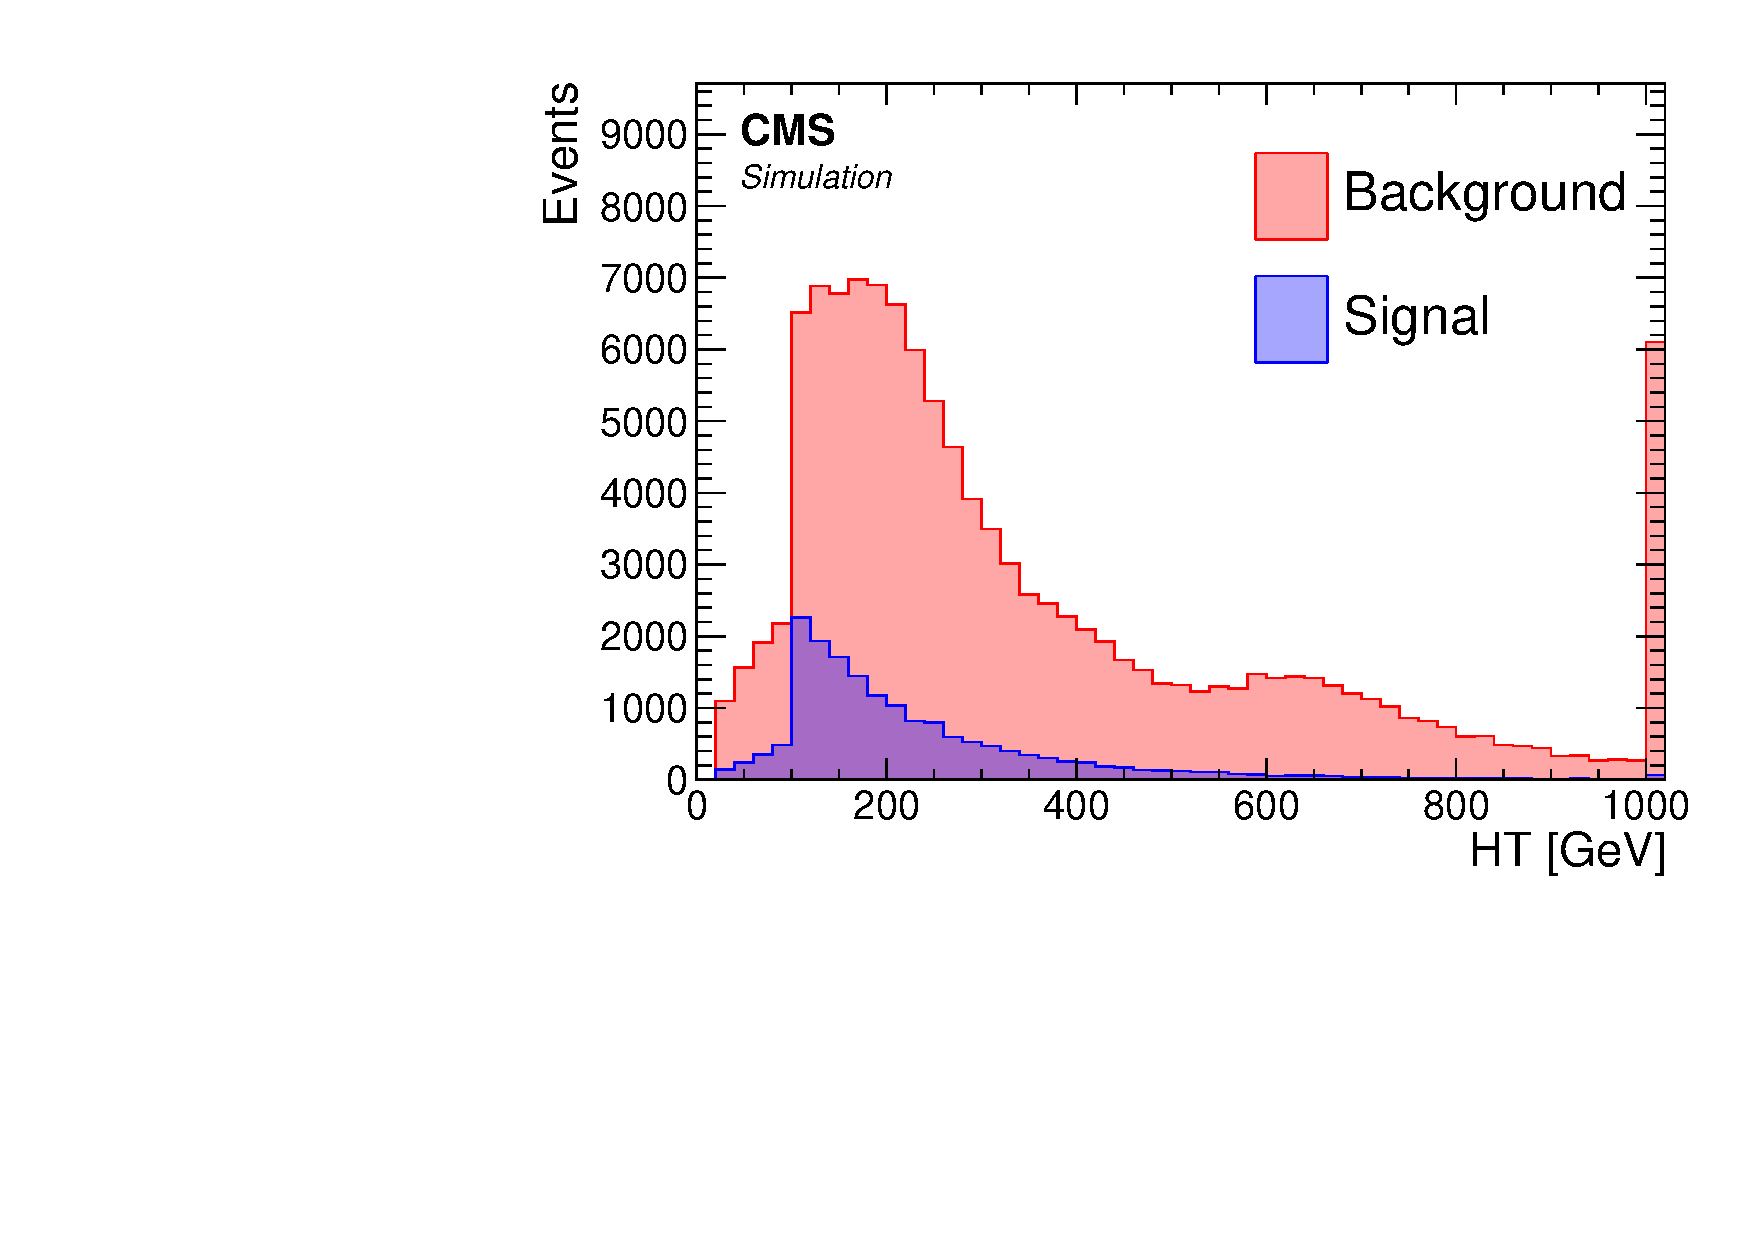
\includegraphics[width=0.32\linewidth]{plots/extrack_bdt_inputs_muons/none_HT.pdf} \,
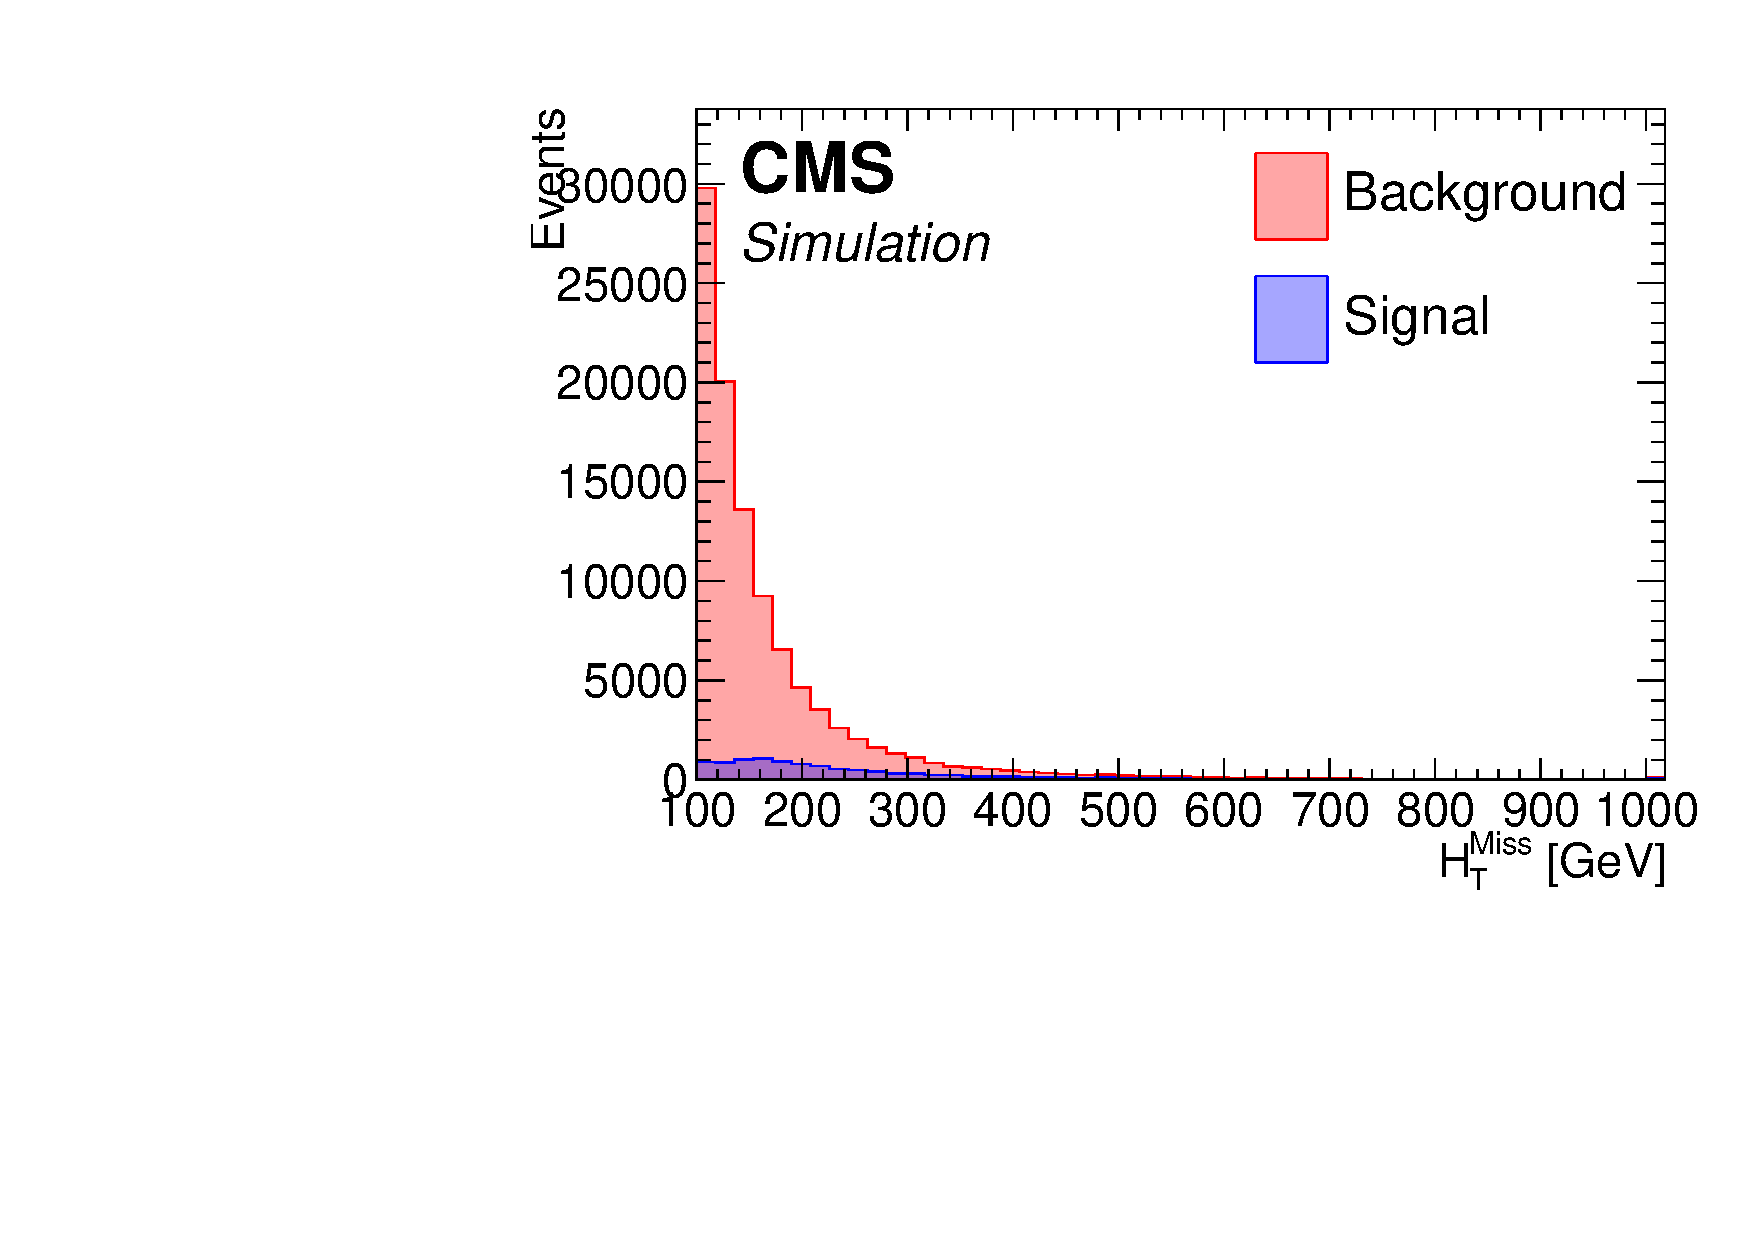
\includegraphics[width=0.32\linewidth]{plots/extrack_bdt_inputs_muons/none_MHT.pdf}  \,
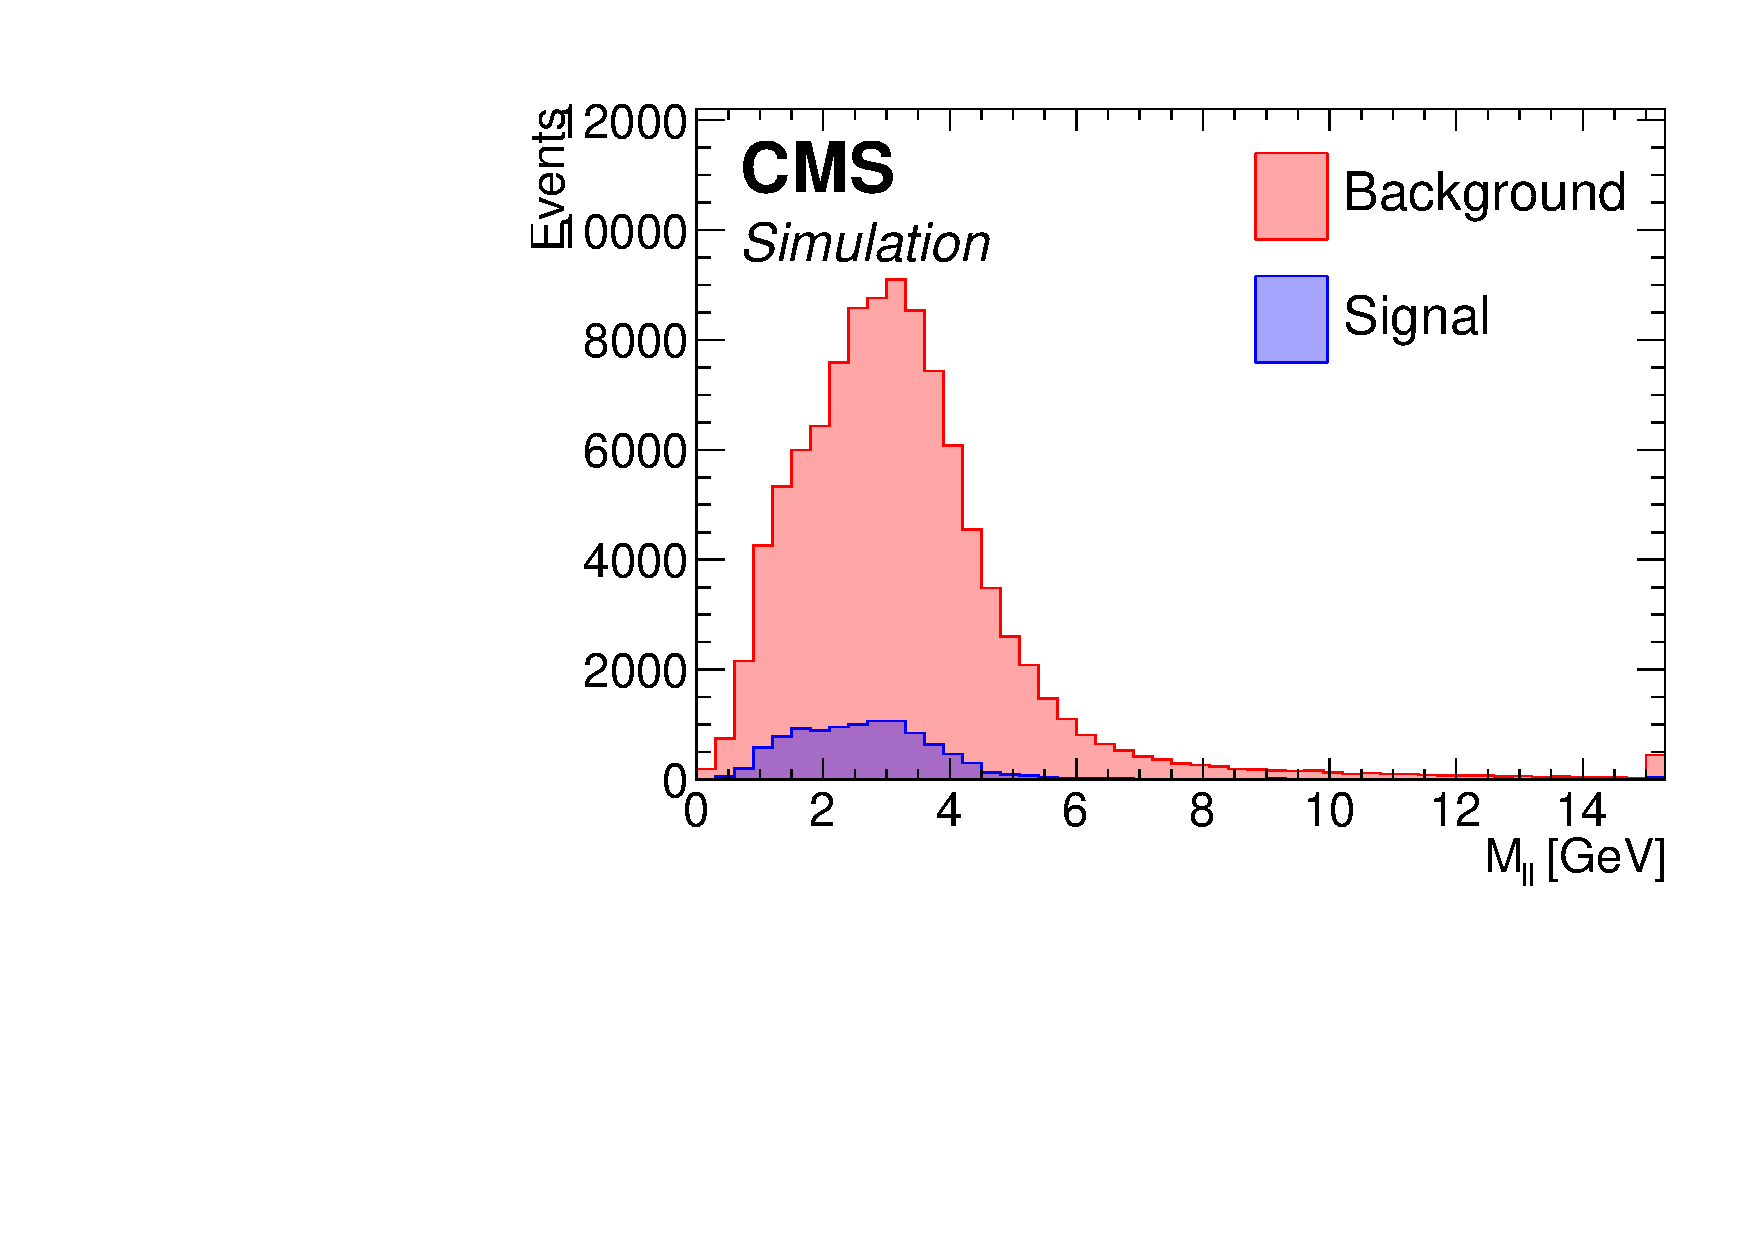
\includegraphics[width=0.32\linewidth]{plots/extrack_bdt_inputs_muons/none_exTrack_invMassCorrJetNoMultIso10Dr0.6.pdf} \\


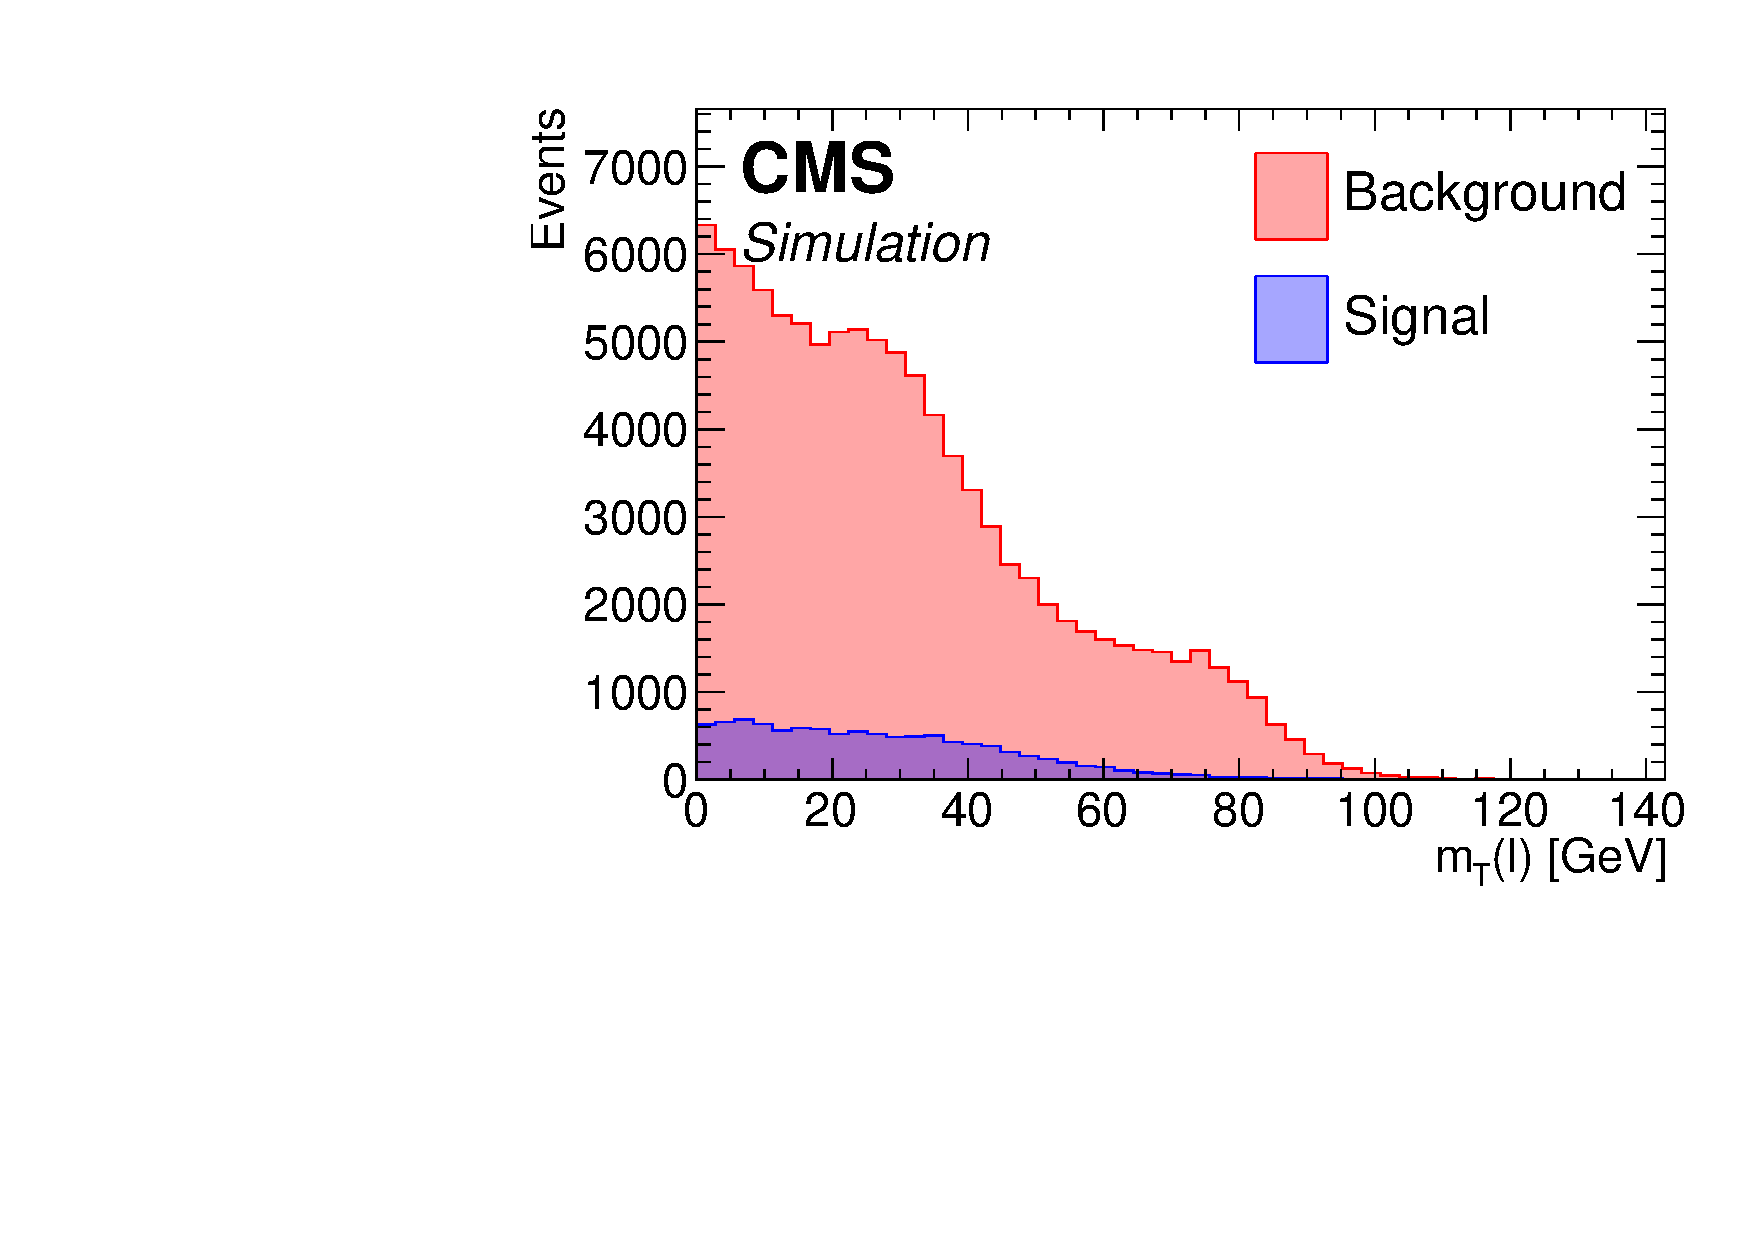
\includegraphics[width=0.32\linewidth]{plots/extrack_bdt_inputs_muons/none_mtlCorrJetNoMultIso10Dr0.6.pdf} \,
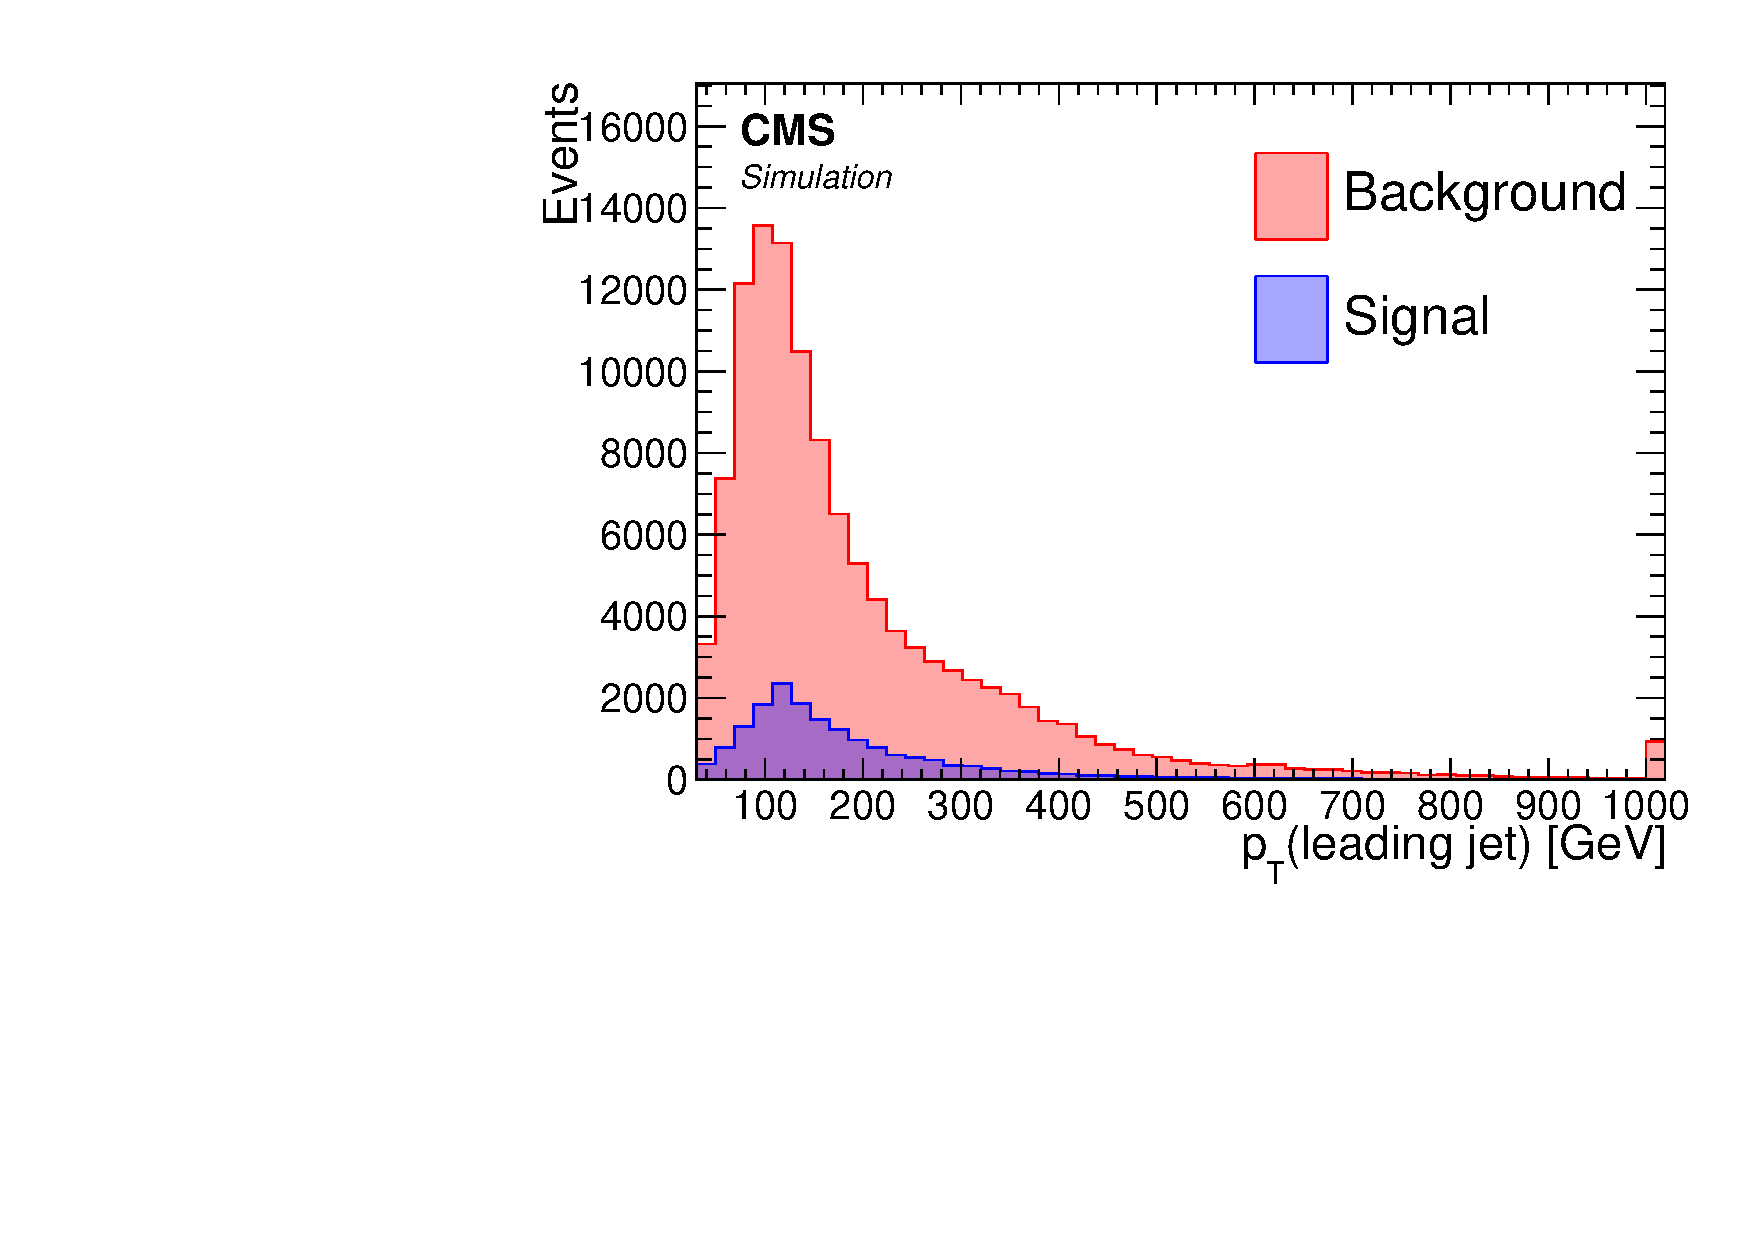
\includegraphics[width=0.32\linewidth]{plots/extrack_bdt_inputs_muons/none_LeadingJetPt.pdf} \,
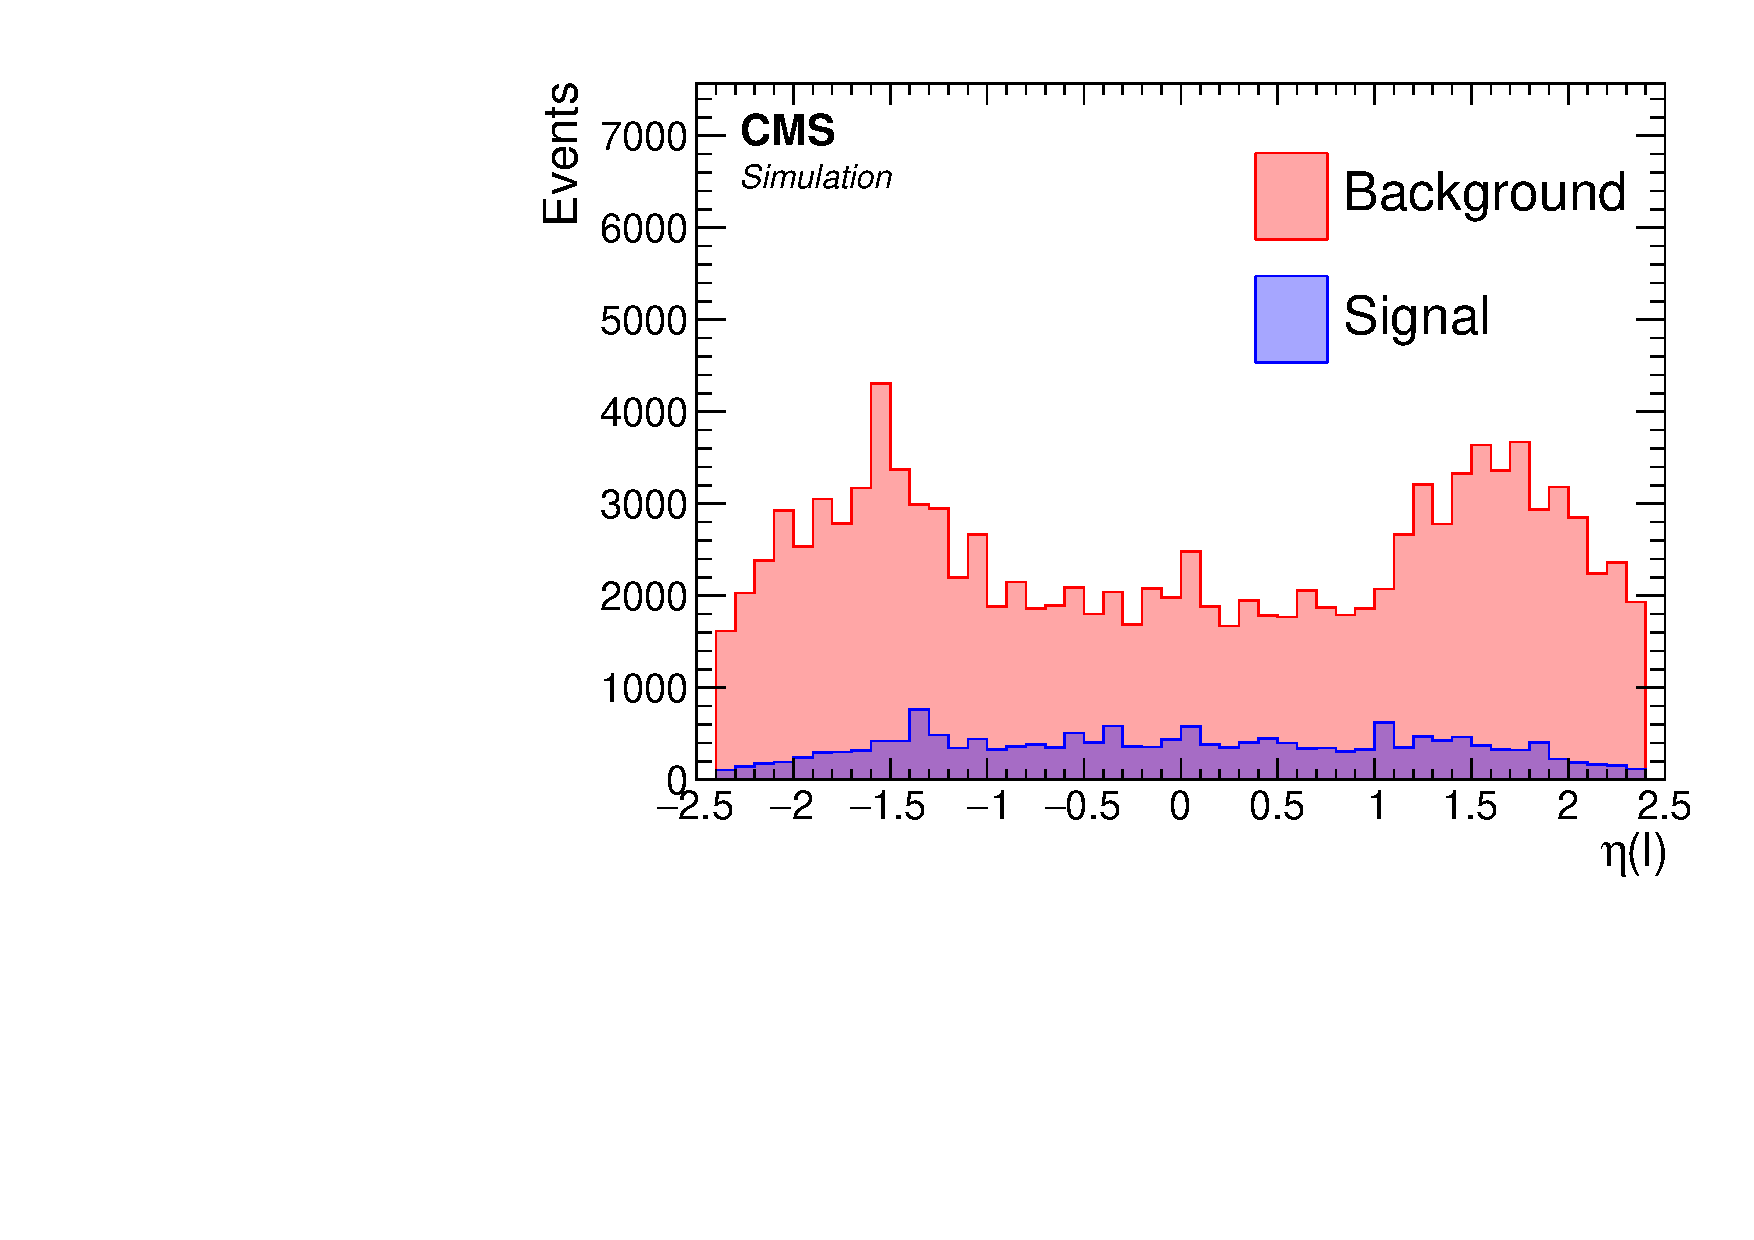
\includegraphics[width=0.32\linewidth]{plots/extrack_bdt_inputs_muons/none_leptonCorrJetNoMultIso10Dr0.6.Eta__.pdf}   \\
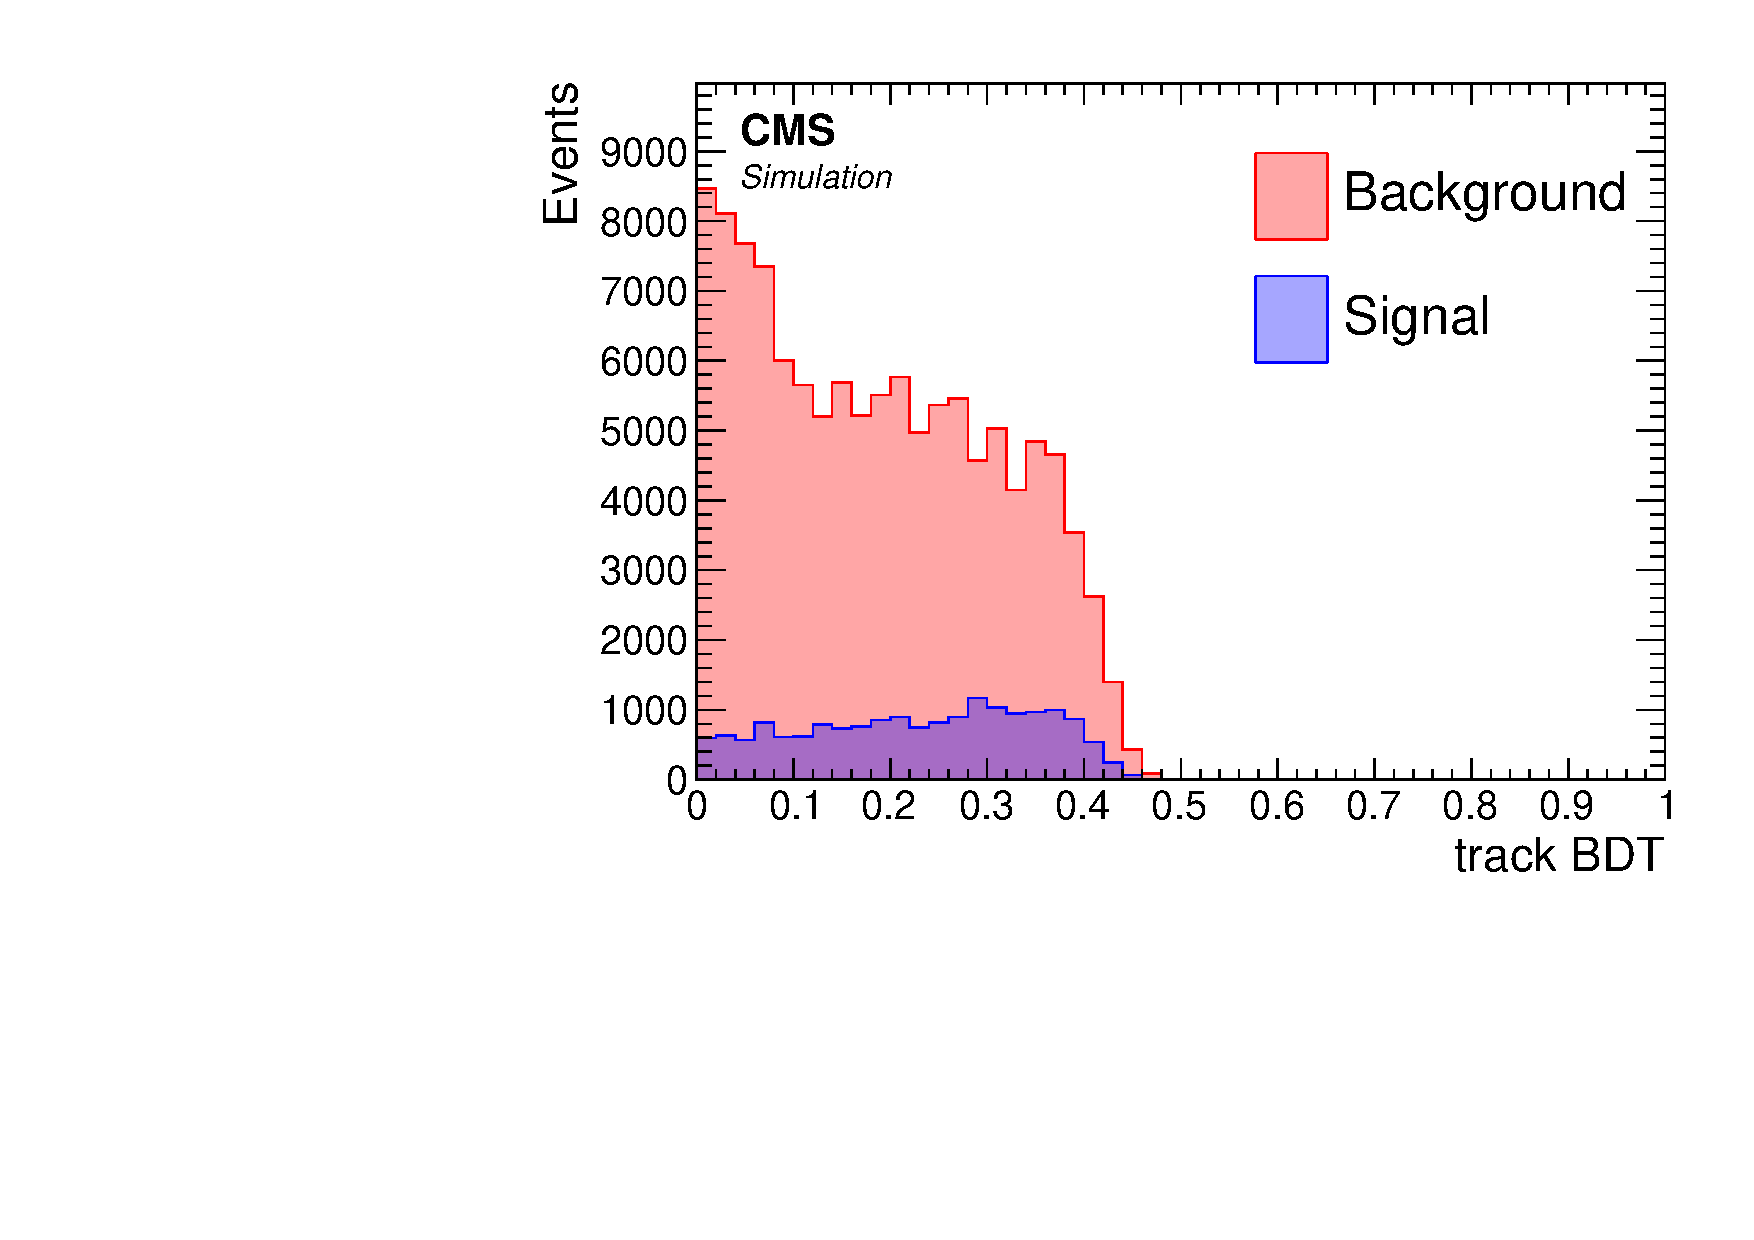
\includegraphics[width=0.32\linewidth]{plots/extrack_bdt_inputs_muons/none_trackBDTCorrJetNoMultIso10Dr0.6.pdf} \,
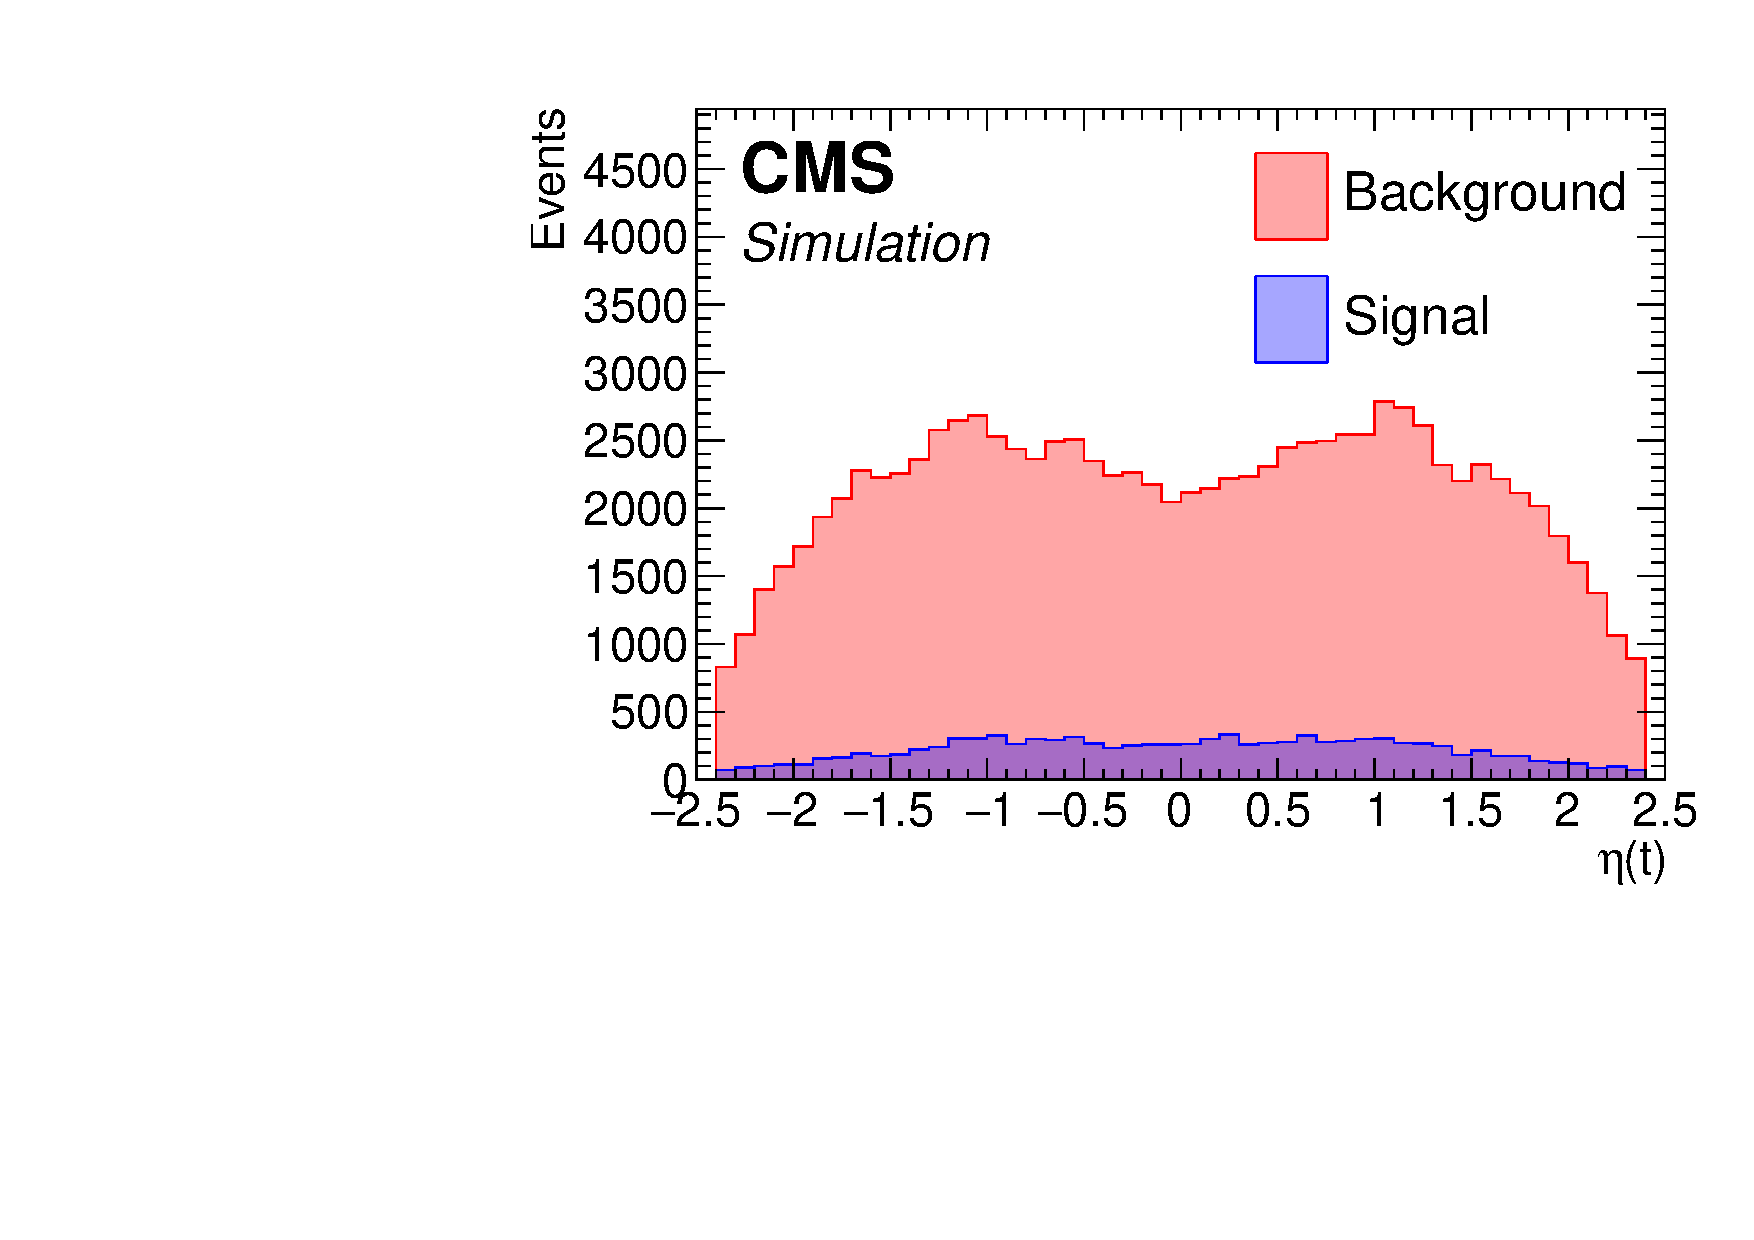
\includegraphics[width=0.32\linewidth]{plots/extrack_bdt_inputs_muons/none_trackCorrJetNoMultIso10Dr0.6.Eta__.pdf}  \,
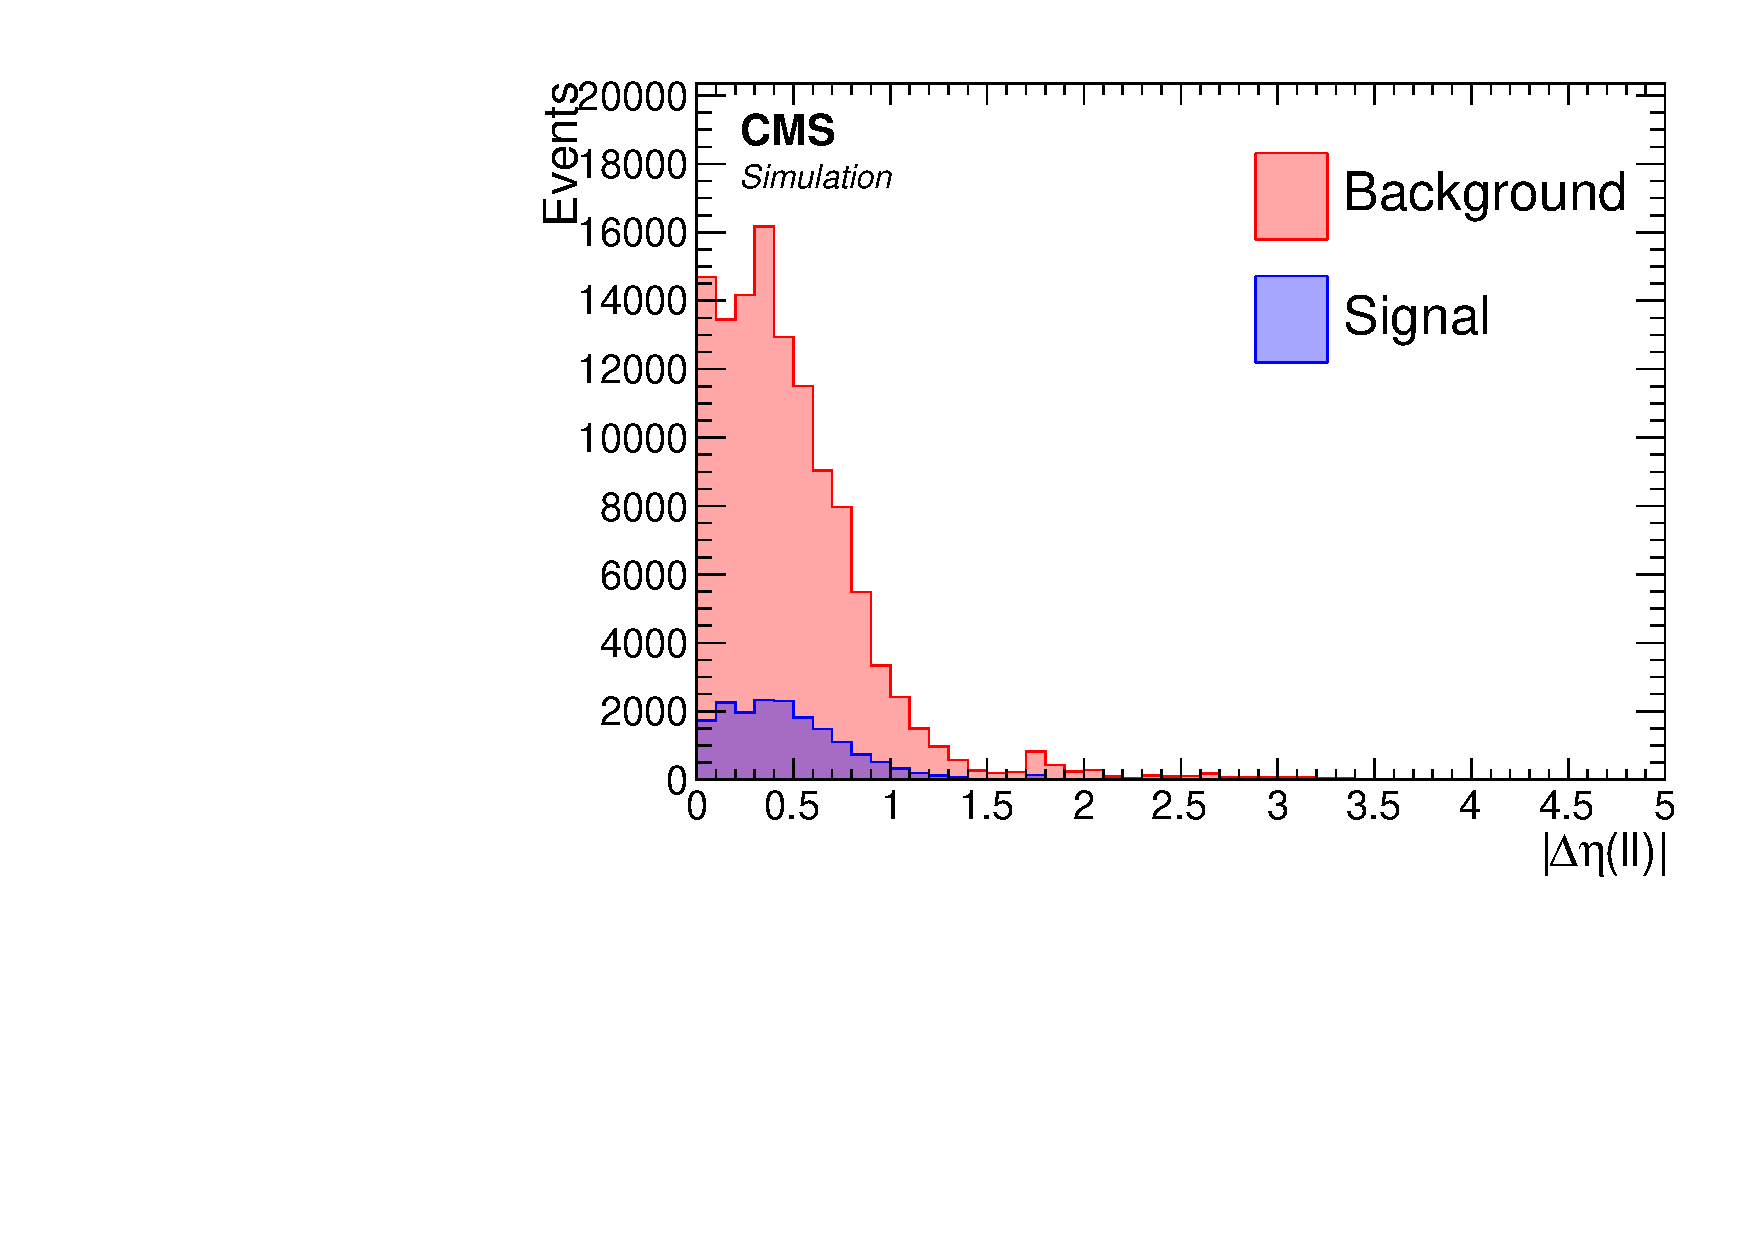
\includegraphics[width=0.32\linewidth]{plots/extrack_bdt_inputs_muons/none_exTrack_deltaEtaCorrJetNoMultIso10Dr0.6.pdf} \\


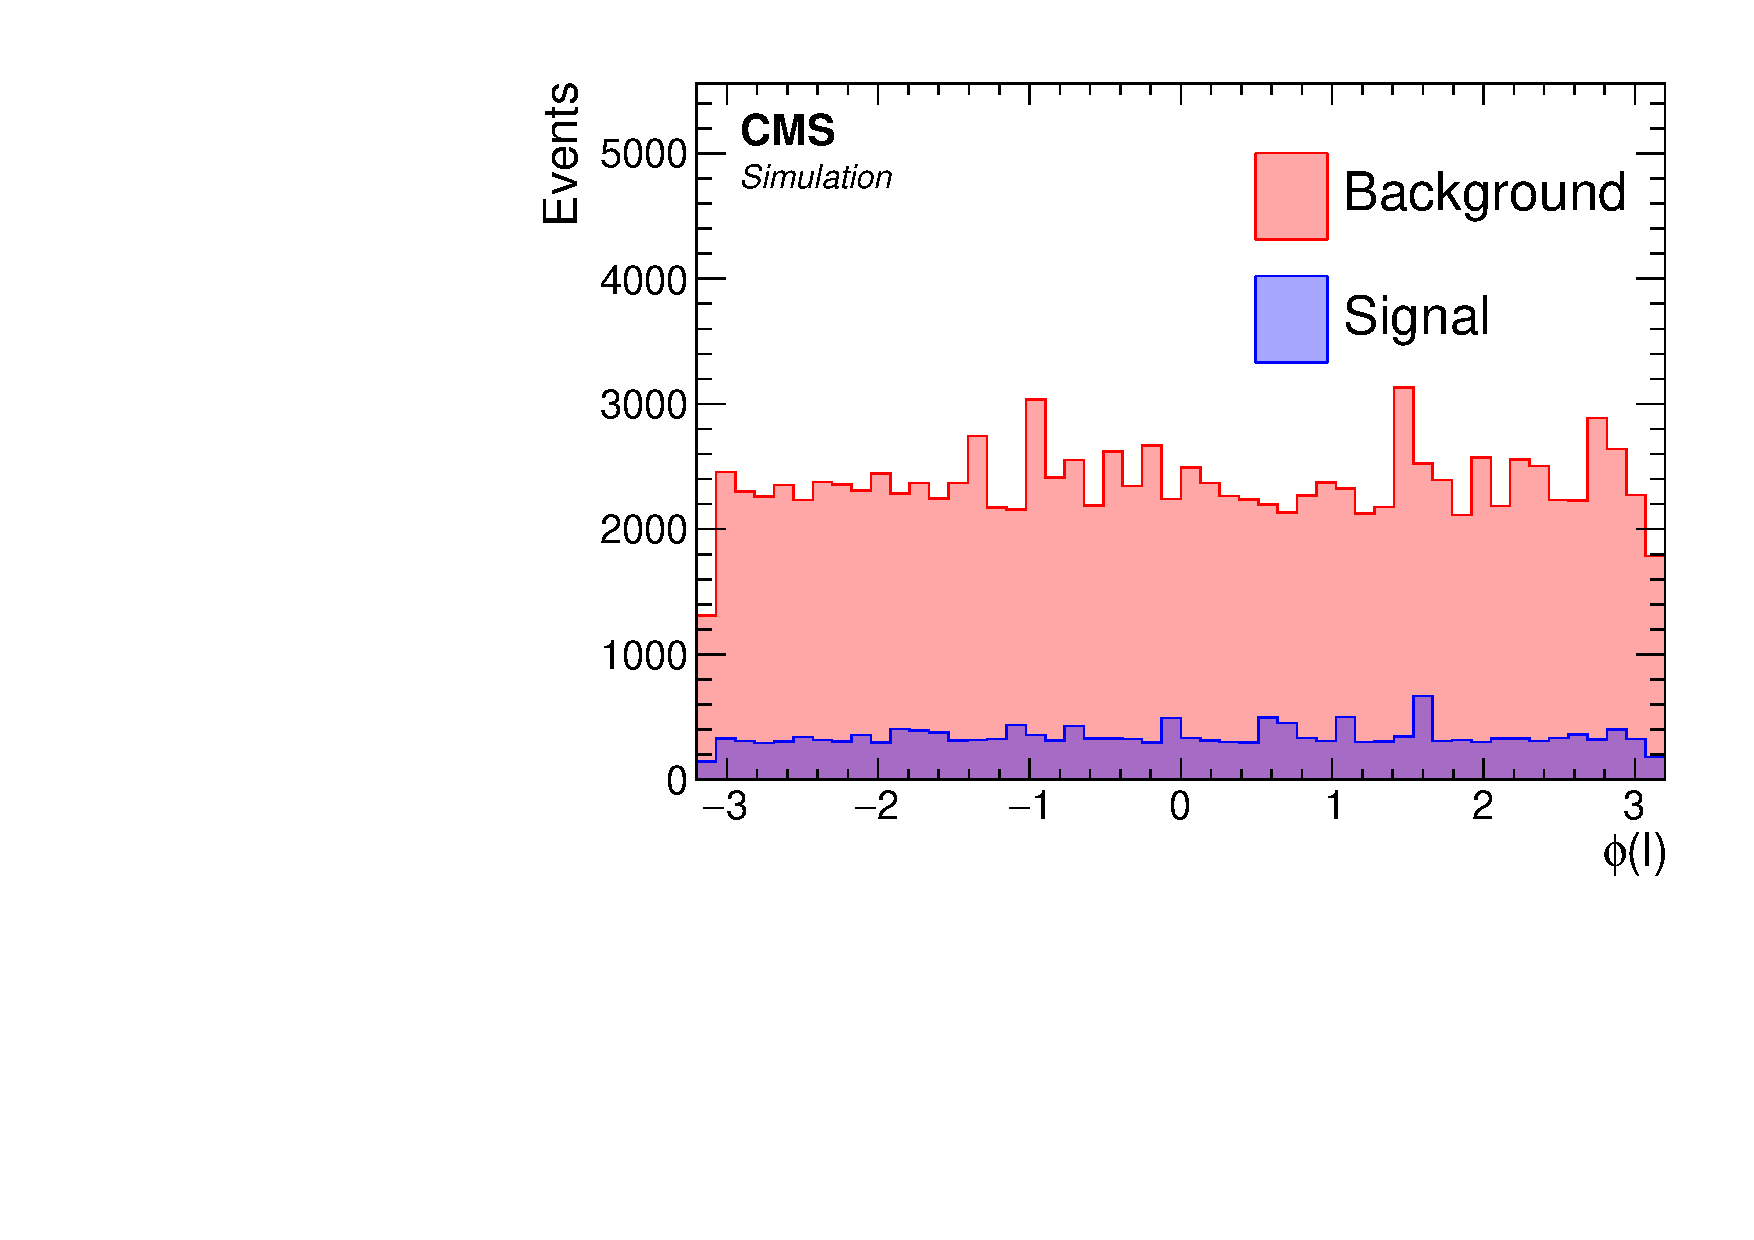
\includegraphics[width=0.32\linewidth]{plots/extrack_bdt_inputs_muons/none_leptonCorrJetNoMultIso10Dr0.6.Phi__.pdf} \,
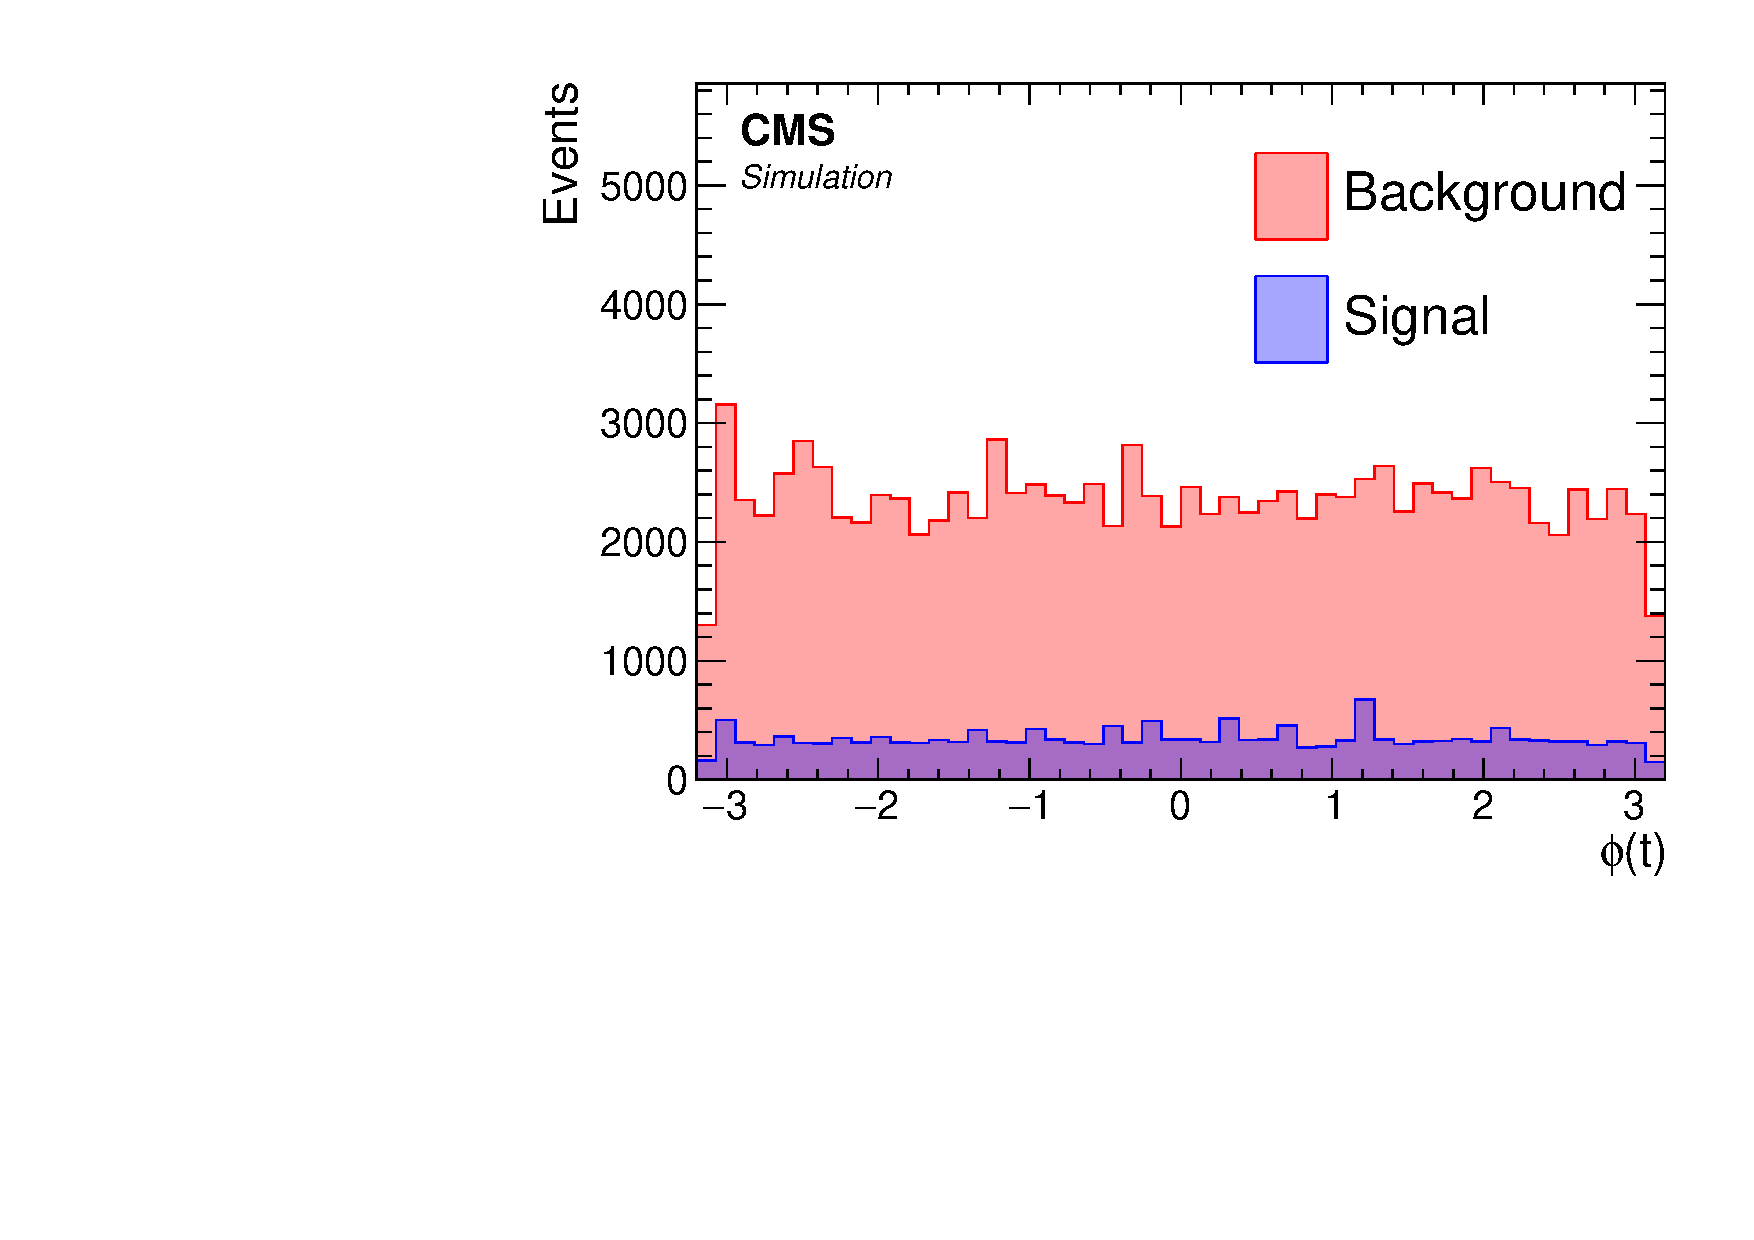
\includegraphics[width=0.32\linewidth]{plots/extrack_bdt_inputs_muons/none_trackCorrJetNoMultIso10Dr0.6.Phi__.pdf} \,
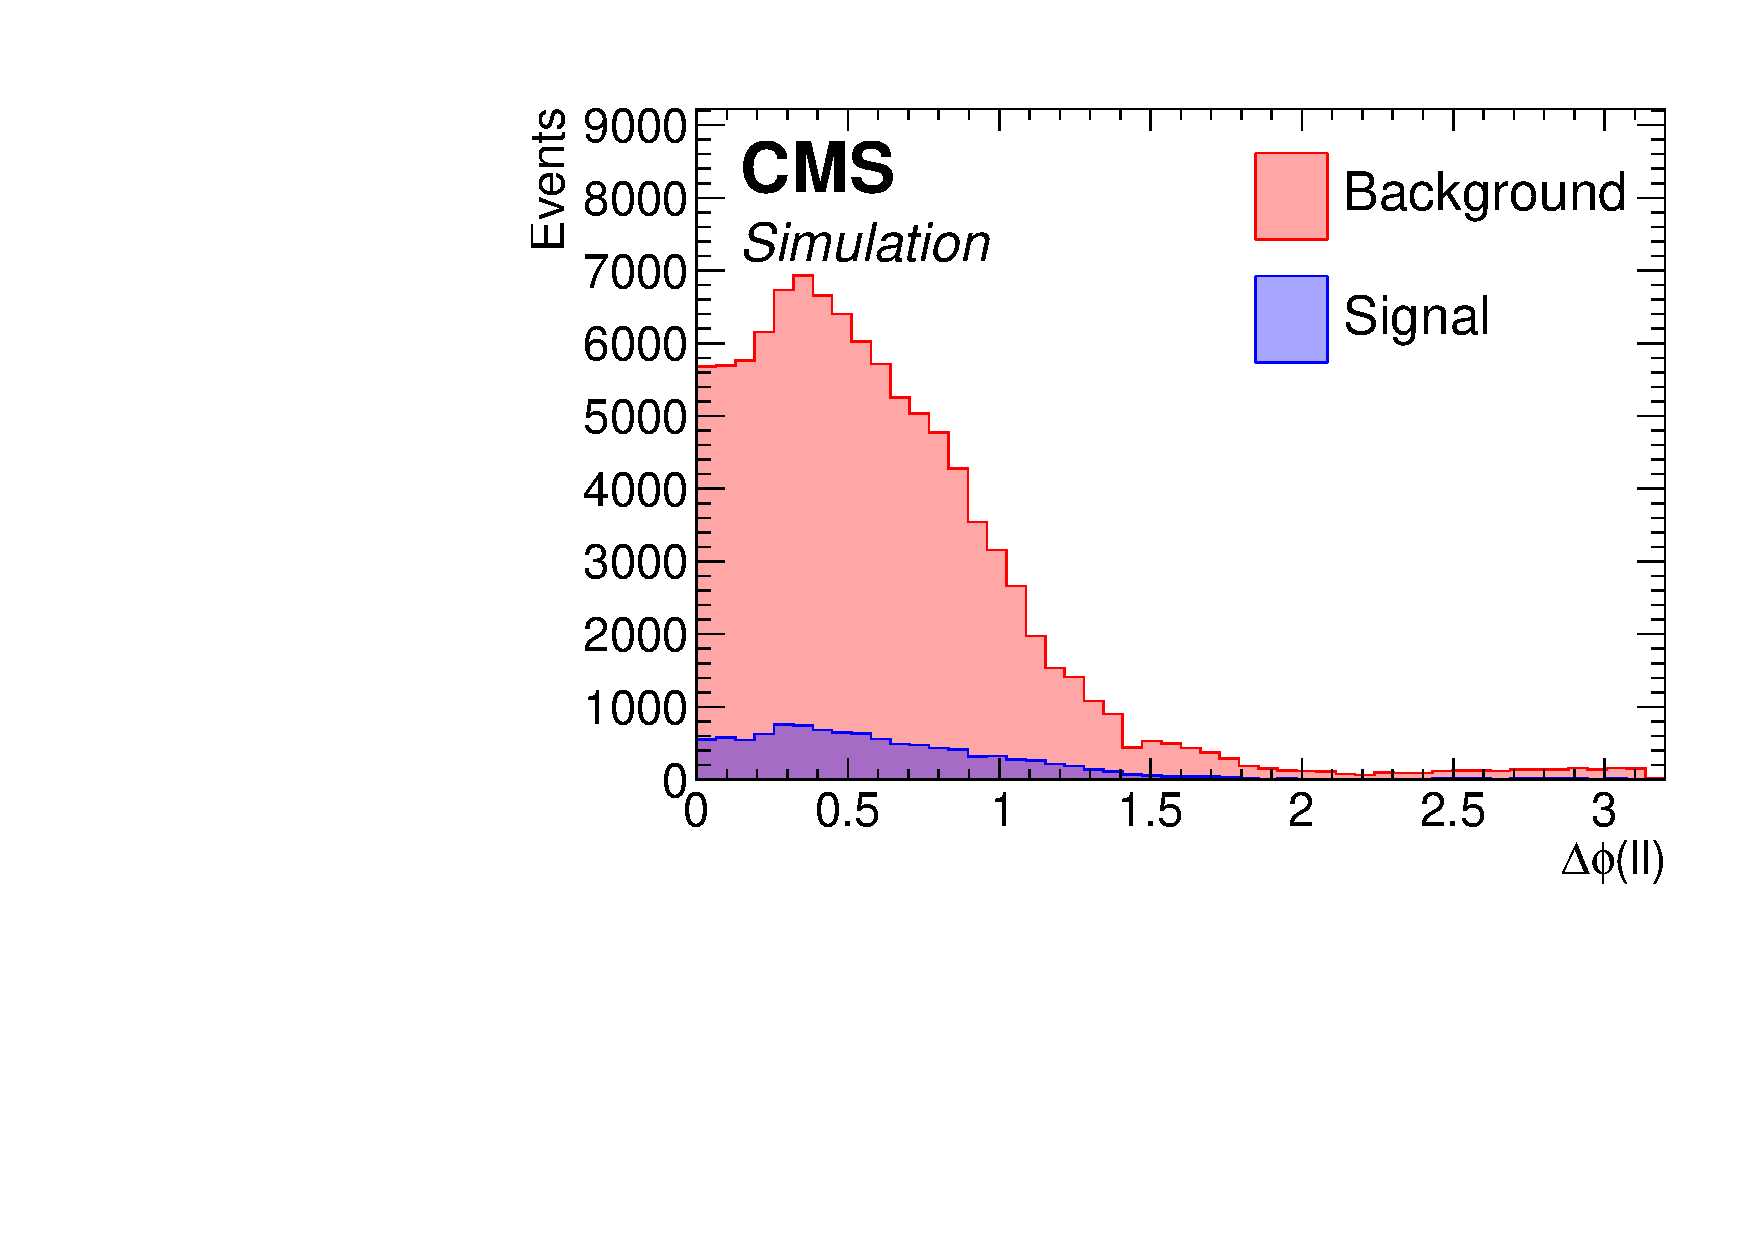
\includegraphics[width=0.32\linewidth]{plots/extrack_bdt_inputs_muons/none_exTrack_deltaPhiCorrJetNoMultIso10Dr0.6.pdf} \\
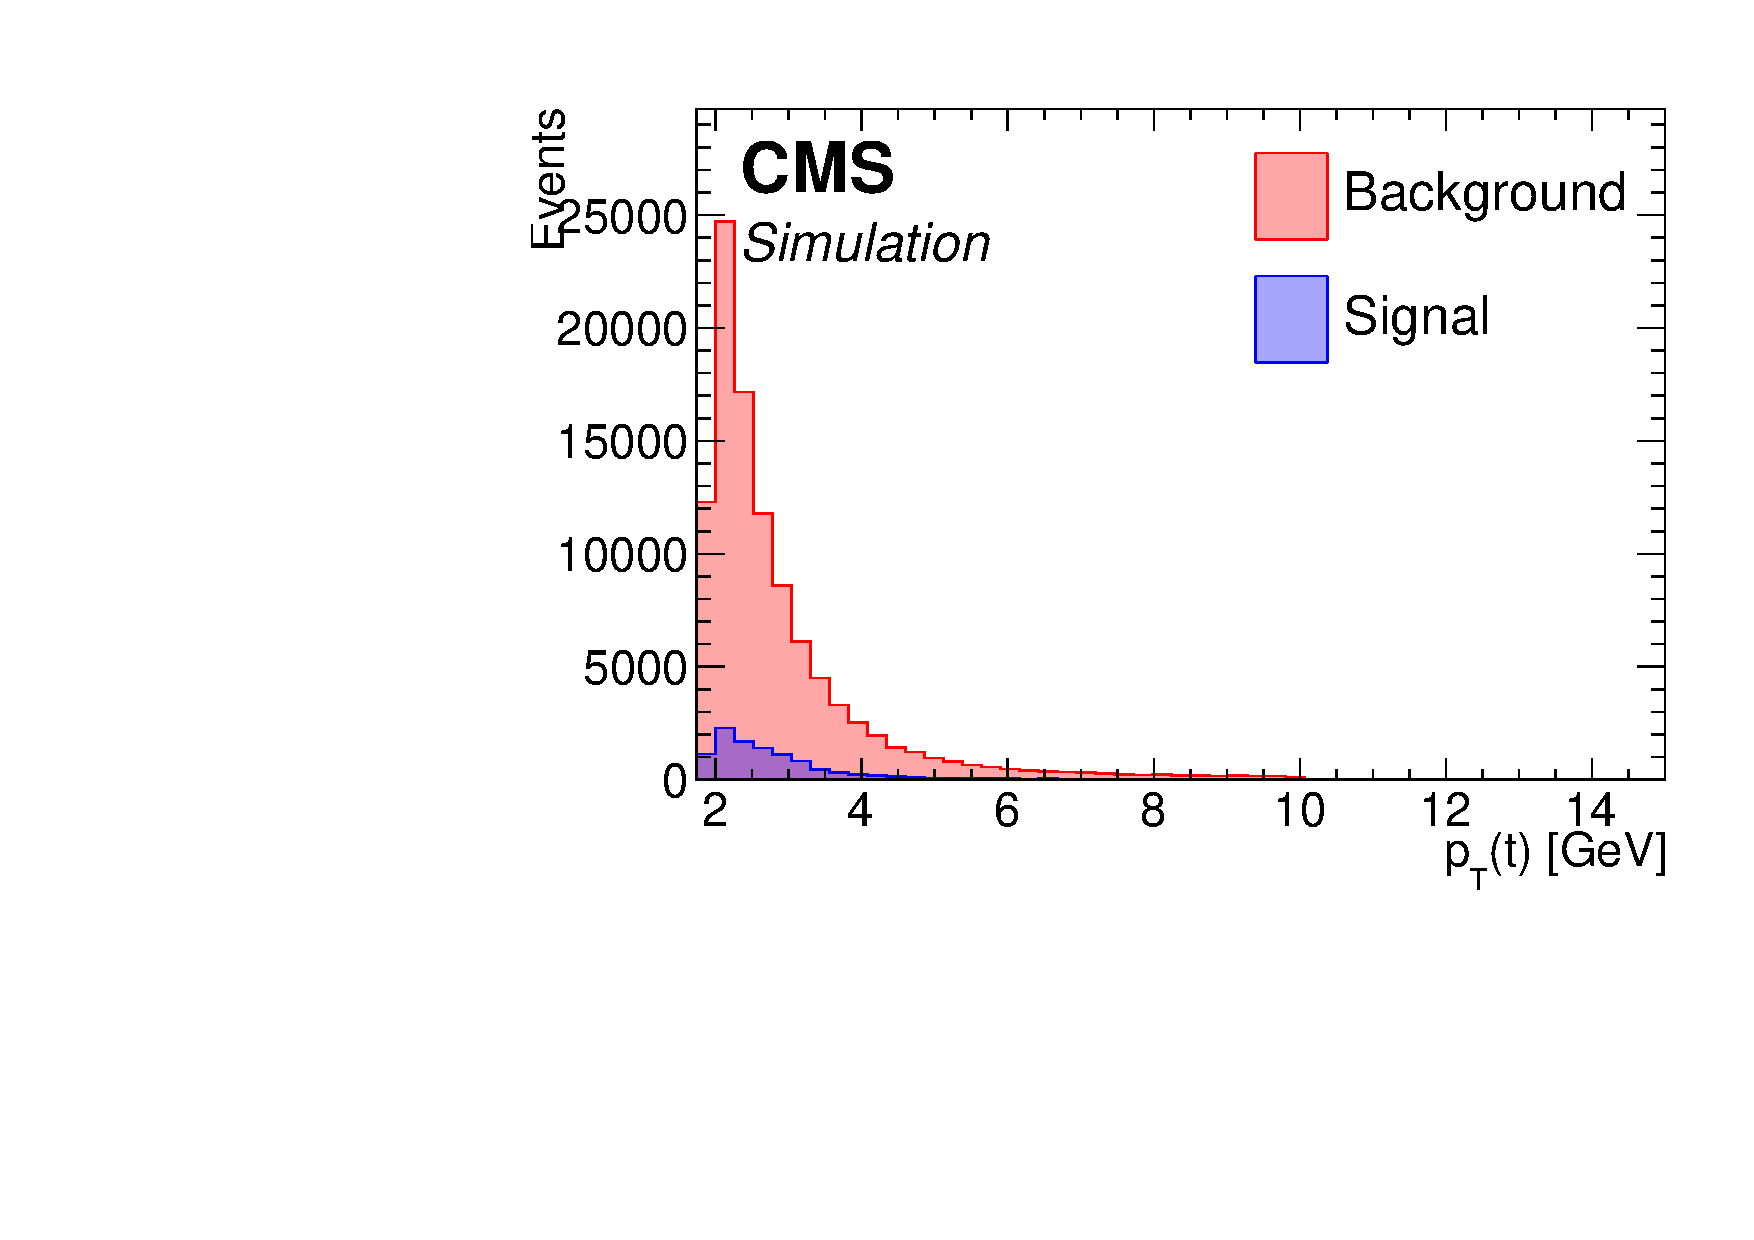
\includegraphics[width=0.32\linewidth]{plots/extrack_bdt_inputs_muons/none_trackCorrJetNoMultIso10Dr0.6.Pt__ .pdf}  \,
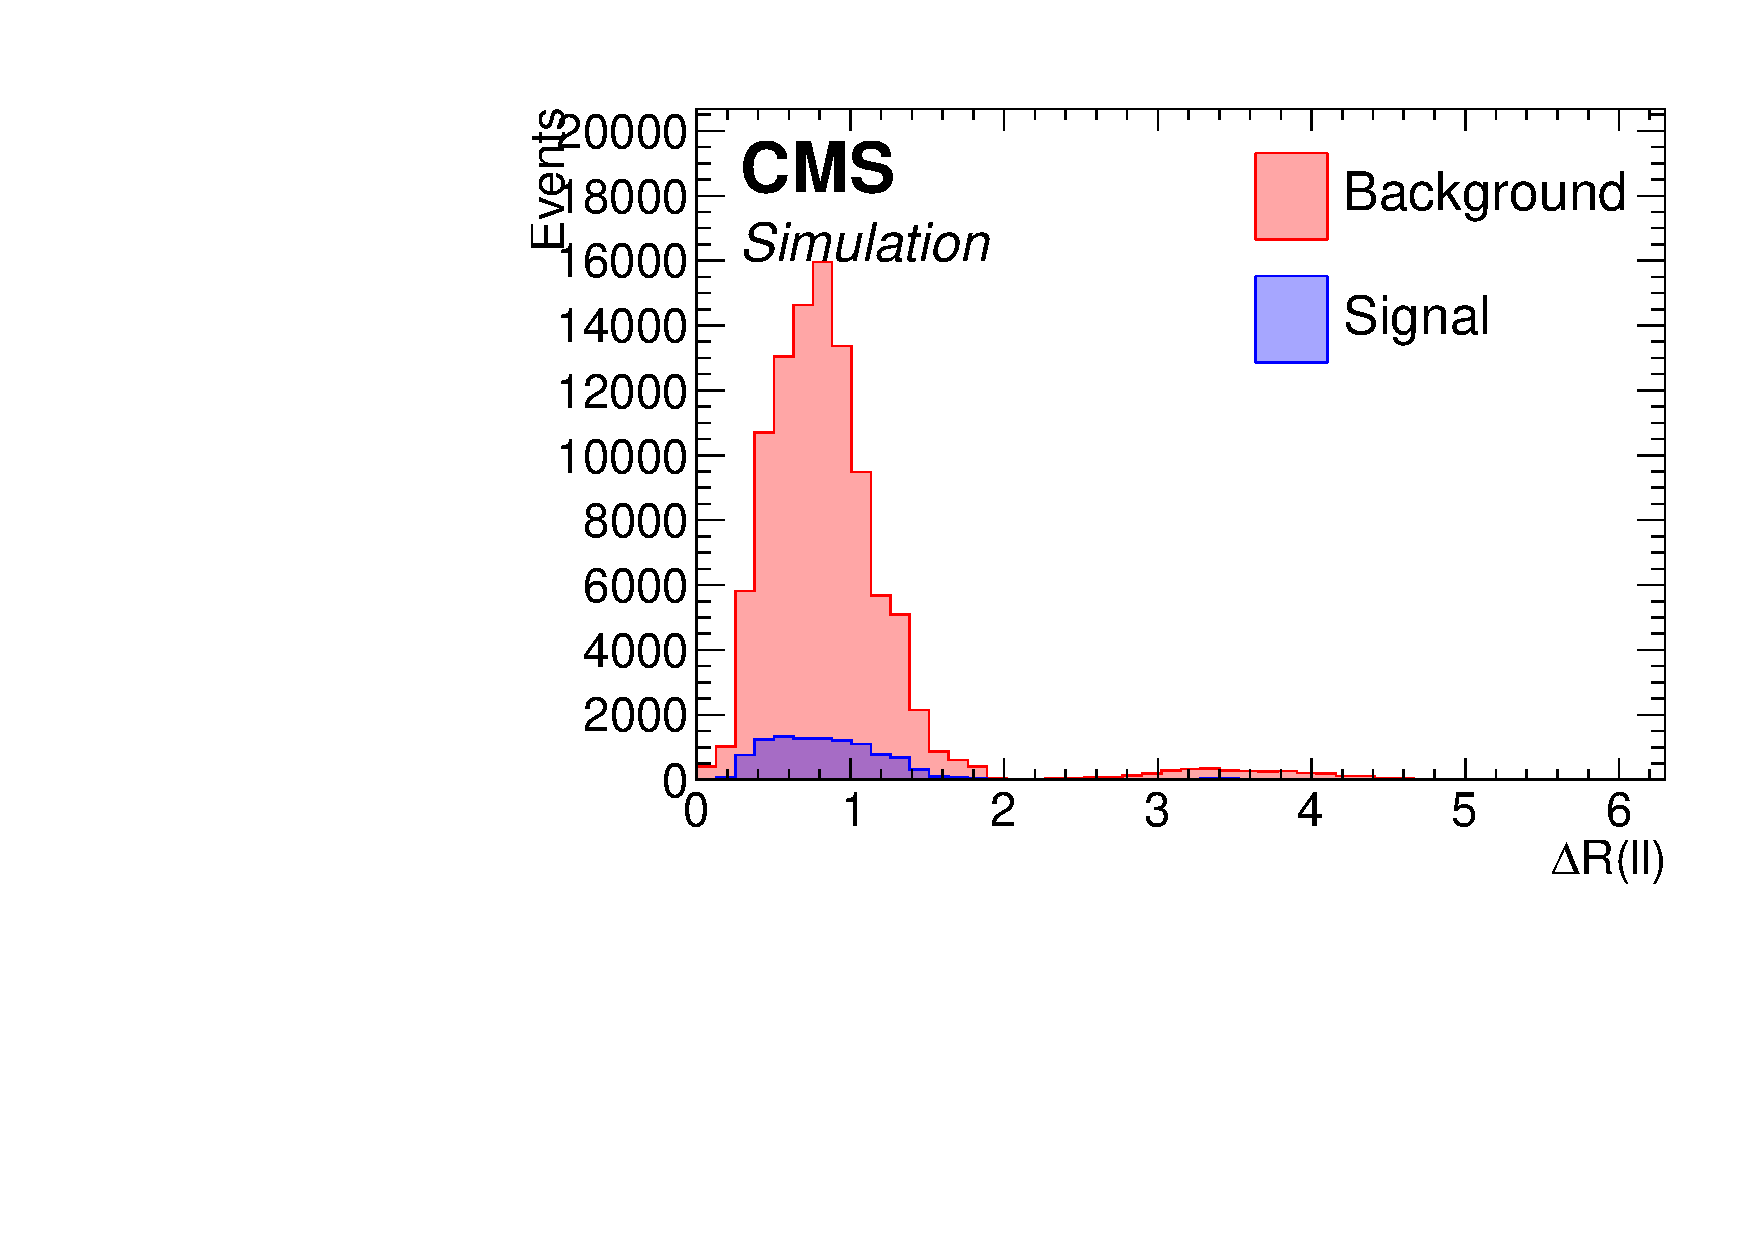
\includegraphics[width=0.32\linewidth]{plots/extrack_bdt_inputs_muons/none_exTrack_deltaRCorrJetNoMultIso10Dr0.6.pdf} \,
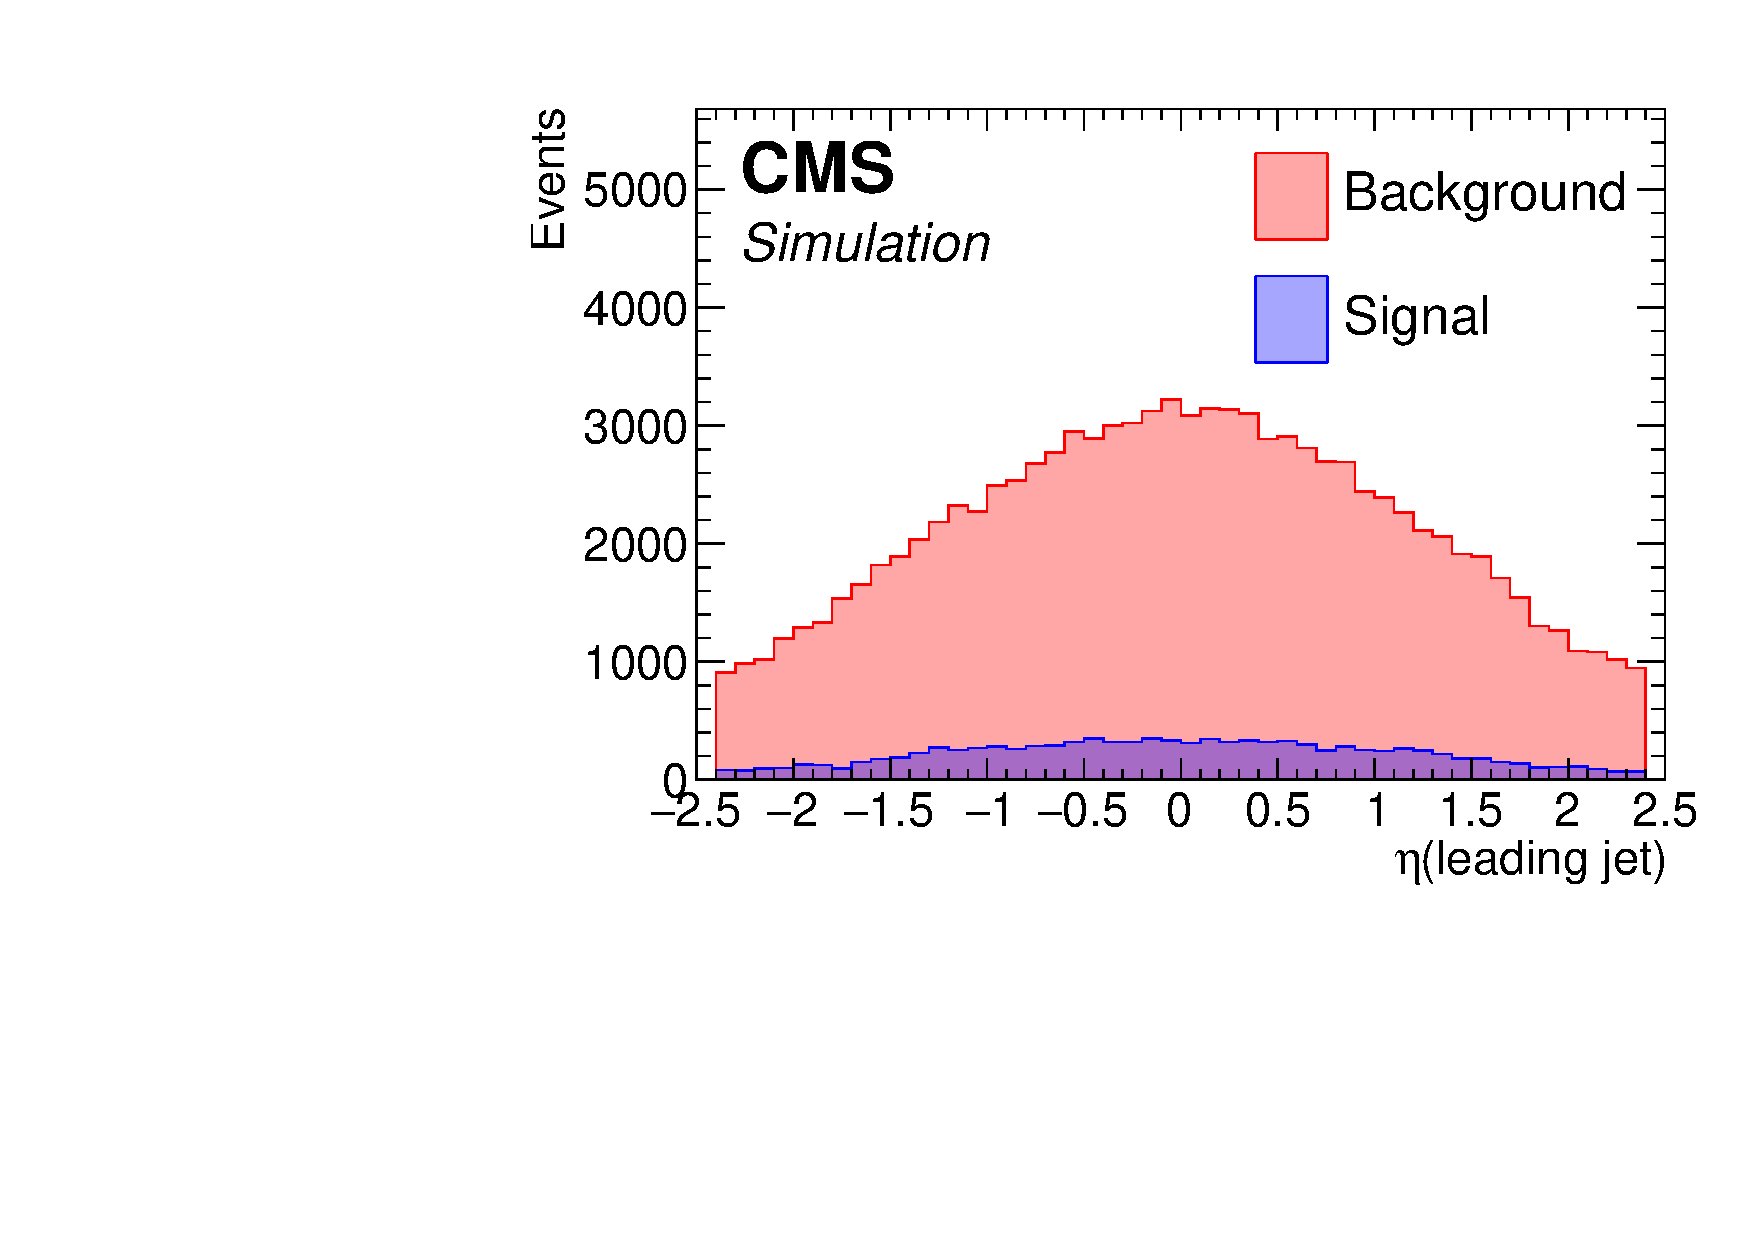
\includegraphics[width=0.32\linewidth]{plots/extrack_bdt_inputs_muons/none_LeadingJet.Eta__.pdf}   \\

\caption[exclusive track training input distribution]{Exclusive track BDT training input variables. Ordered by importance ranking.}
\label{fig:extrack-input-distributions}
\end{figure}